\documentclass[ece,thesis]{puthesis}

\usepackage{amsmath}
\usepackage{multicol}
%\usepackage{subfigure}

%from start
\usepackage{amssymb}
\usepackage{float}
\usepackage{hhline}
\usepackage{multirow}
\usepackage{color,graphicx}
\usepackage{hyperref}
%from end

% add 6/5/2018
\usepackage{mhchem}

% add 6/12/2018
\floatstyle{plaintop}
\restylefloat{table}

% add 6/25/2018
\usepackage{subcaption}

% add 7/1/2018
\usepackage{pdflscape}

% add 7/18/2018
\usepackage{setspace}
\usepackage[labelsep=space]{caption}



\title{Development of a Single-Ended Laser-Absorption Spectroscopy Sensor for High-Temperature Gases}
\author{Yuzhe Zhou}{Zhou, Yuzhe}
\pudegree{Master of Science in Mechanical Engineering}{M.S.M.E.}{August}{2018}

\majorprof{Christopher S. Goldenstein, School of Mechanical Engineering}
\campus{West Lafayette}

%
%  mydefs.tex  2007-03-19  Mark Senn  http://www.ecn.purdue.edu/~mark
%
%  Command definitions that can be used in all documents that have
%      %
%  mydefs.tex  2007-03-19  Mark Senn  http://www.ecn.purdue.edu/~mark
%
%  Command definitions that can be used in all documents that have
%      %
%  mydefs.tex  2007-03-19  Mark Senn  http://www.ecn.purdue.edu/~mark
%
%  Command definitions that can be used in all documents that have
%      \input{mydefs}
%

% CHANGE NEXT 3 LINES?
% Define \be and \ee to start and end the equation environment.
\newcommand{\be}{\begin{equation}}
\newcommand{\ee}{\end{equation}}

% CHANGE NEXT 12 LINES?
% Define \Repeat so, for example,
%     \Repeat{whatever}{10}
% is the same as typing whatever 10 times.
\newcount{\myi}
\newcommand{\Repeat}[2]{%
    \myi=0
    \loop
        \ifnum\myi<#2
        #1
        \advance\myi by 1
    \repeat
}

% CHANGE NEXT 3 LINES?
% Make "\Sum ab" or "\Sum{a}{b}" do "\sum_{a}^{b}".
% This can only be used when in math mode.
\newcommand\Sum[2]{\sum_{#1}^{#2}}

% CHANGE NEXT 4 LINES?
% Make "\xn" do "$x_n$".
% Because this definition contains the "$" to go into math mode
% this definition must be used when not in math mode.
\newcommand{\xn}{$x_n$}

% CHANGE NEXT 5 LINES?
% Since \xn is already defined we must use \renewcommand to redefine it.
% Normally you would not have the above definition for \xn in this file
% if you were just going to override it later.
% The \ensuremath goes into math mode if not already in math mode.
\renewcommand{\xn}{\ensuremath{x_n}}
%

% CHANGE NEXT 3 LINES?
% Define \be and \ee to start and end the equation environment.
\newcommand{\be}{\begin{equation}}
\newcommand{\ee}{\end{equation}}

% CHANGE NEXT 12 LINES?
% Define \Repeat so, for example,
%     \Repeat{whatever}{10}
% is the same as typing whatever 10 times.
\newcount{\myi}
\newcommand{\Repeat}[2]{%
    \myi=0
    \loop
        \ifnum\myi<#2
        #1
        \advance\myi by 1
    \repeat
}

% CHANGE NEXT 3 LINES?
% Make "\Sum ab" or "\Sum{a}{b}" do "\sum_{a}^{b}".
% This can only be used when in math mode.
\newcommand\Sum[2]{\sum_{#1}^{#2}}

% CHANGE NEXT 4 LINES?
% Make "\xn" do "$x_n$".
% Because this definition contains the "$" to go into math mode
% this definition must be used when not in math mode.
\newcommand{\xn}{$x_n$}

% CHANGE NEXT 5 LINES?
% Since \xn is already defined we must use \renewcommand to redefine it.
% Normally you would not have the above definition for \xn in this file
% if you were just going to override it later.
% The \ensuremath goes into math mode if not already in math mode.
\renewcommand{\xn}{\ensuremath{x_n}}
%

% CHANGE NEXT 3 LINES?
% Define \be and \ee to start and end the equation environment.
\newcommand{\be}{\begin{equation}}
\newcommand{\ee}{\end{equation}}

% CHANGE NEXT 12 LINES?
% Define \Repeat so, for example,
%     \Repeat{whatever}{10}
% is the same as typing whatever 10 times.
\newcount{\myi}
\newcommand{\Repeat}[2]{%
    \myi=0
    \loop
        \ifnum\myi<#2
        #1
        \advance\myi by 1
    \repeat
}

% CHANGE NEXT 3 LINES?
% Make "\Sum ab" or "\Sum{a}{b}" do "\sum_{a}^{b}".
% This can only be used when in math mode.
\newcommand\Sum[2]{\sum_{#1}^{#2}}

% CHANGE NEXT 4 LINES?
% Make "\xn" do "$x_n$".
% Because this definition contains the "$" to go into math mode
% this definition must be used when not in math mode.
\newcommand{\xn}{$x_n$}

% CHANGE NEXT 5 LINES?
% Since \xn is already defined we must use \renewcommand to redefine it.
% Normally you would not have the above definition for \xn in this file
% if you were just going to override it later.
% The \ensuremath goes into math mode if not already in math mode.
\renewcommand{\xn}{\ensuremath{x_n}}
\newcommand{\margins}{\Repeat{Show where the margins for the page are.}{4}}
\let\en=\ensuremath
\newcommand{\ve}[2]{\en{#1_1},~\en{#1_2},\ \ldots,~\en{#1_{#2}}}

\begin{document}

\volume

% Front matter (dedication, etc.).
%
%  This is ``front matter'' for the thesis.
%
%  Regarding ``References'' below:
%      KEY    MEANING
%      PU     ``A Manual for the Preparation of Graduate Theses'',
%             The Graduate School, Purdue University, 1996.
%      PU8    ``A Manual for the Preparation of Graduate Theses'',
%             Eighth Revise Edition, Purdue University.
%      TCMOS  The Chicago Manual of Style, Edition 14.
%      WNNCD  Webster's Ninth New Collegiate Dictionary.
%
%  Lines marked with "%%" may need to be changed.
%

  % Statement of Thesis/Dissertation Approval Page
  % This page is REQUIRED.  The page should be numbered page ``ii''
  % and should NOT be listed in your TABLE OF CONTENTS.
  % References: PU8 ordinal pages 5 and 29.
  % The web page https://engineering.purdue.edu/AAE retrieved on
  % January 8, 2017 had "School of Aeronautics and Astronautics"---that
  % is used instead of "Department af Aeronautics and Astronautics"
  % below.
\begin{statement}
  \entry{Dr.~Christopher S. Goldenstein, Chair}{School of Mechanical Engineering}
  \entry{Dr.~Gregory M. Shaver}{School of Mechanical Engineering}
  \entry{Dr.~Terrence R. Meyer}{School of Mechanical Engineering}
  \approvedby{Dr.~Jay P. Gore}{Director of Graduate Programs}
\end{statement}

  % Dedication page is optional.
  % A name and often a message in tribute to a person or cause.
  % References: PU 15, WNNCD 332.
\begin{dedication}
For my parents
\end{dedication}

\begin{acknowledgments}
Throughout my academic journey, I have been so lucky to receive support from my family, friends, colleagues and mentors. Without their help I couldn't have achieved all that I have.

I would like to first give my most sincere gratitude to my advisor, Prof. Chris Goldenstein, for bringing me to Purdue and providing me with great research opportunities throughout the time. Not only has he offered patient guidance with incredible inspiration and insight, but more importantly, he encouraged and taught me to keep being diligent and pursuing great excellence in research and life. Although I am still far away from that, I will keep it in my mind for the rest of my journey of life. I appreciate the opportunity Prof. Gregory Shaver has given me to take measurements in his engine in the Herrick Laboratories and for serving on my committee. I also thank Prof. Terrence Meyer for serving on my committee. 

I have also spent a great time exploring new things with my dear friends and working with fantastic fellow engineers. The students of the Goldenstein Group (Ryan Tancin, Garrett Mathews, Morgan Ruesch and Austin McDonald) share a great deal of incredible ideas and knowledge. I would like to thank Garrett Mathews for his help and support in my experiment. I also appreciate Dheeraj Gosala for helping me with all kinds of work in Herrick.

Finally but most importantly, I would like to thank my dear parents for their endless love and encouragement. They are always ready for supporting me financially and mentally. My mother created a home of love, and kept imparting her wisdom and a great number of life skills and interpersonal skills to me. My father, also majoring in mechanical engineering, always reminded me of working hard and being aware of what matters most at the present stage. He provided me a lot of visions in the industries, and always encouraged me to go beyond my comfort zone and take up new challenges.

\end{acknowledgments}

  % The preface is optional.
  % References: PU 16, TCMOS 1.49, WNNCD 927.
%\begin{preface}
%  This is the preface.
%\end{preface}

  % The Table of Contents is required.
  % The Table of Contents will be automatically created for you
  % using information you supply in
  %     \chapter
  %     \section
  %     \subsection
  %     \subsubsection
  % commands.
  % Reference: PU 16.
\tableofcontents

  % If your thesis has tables, a list of tables is required.
  % The List of Tables will be automatically created for you using
  % information you supply in
  %     \begin{table} ... \end{table}
  % environments.
  % Reference: PU 16.
\listoftables

  % If your thesis has figures, a list of figures is required.
  % The List of Figures will be automatically created for you using
  % information you supply in
  %     \begin{figure} ... \end{figure}
  % environments.
  % Reference: PU 16.
\listoffigures

  % List of Symbols is optional.
  % Reference: PU 17.
%\begin{symbols}
%  $m$& mass\cr
%  $v$& velocity\cr
%\end{symbols}

  % List of Abbreviations is optional.
  % Reference: PU 17.
%\begin{abbreviations}
%  abbr& abbreviation\cr
%  bcf& billion cubic feet\cr
%  BMOC& big man on campus\cr
%\end{abbreviations}

  % Nomenclature is optional.
  % Reference: PU 17.
\begin{nomenclature}
  $A$& Integrated absorbance\cr
  CAD& Computer aided design\cr
  DA& Direct absorption\cr
  DFB& Distributed-feedback\cr
  DPF& Diesel particulate filter\cr
  $E^"$& Lower-state energy\cr
  $f_m$& Modulation frequency\cr
  $f_s$& Scan frequency\cr
  FTS& Fourier Transform Spectroscopy\cr
  FWHM& Full-width at half-maximum\cr
  $G$& Detector gain\cr
  $h$& Planck's constant\cr
  HCCI& Homogeneous-charge compression ignition\cr
  HWHM& Half-width at half-maximum\cr
  IC& Internal combustion\cr
  $I_0$& Incident laser light intensity\cr
  $I_t$& Transmitted laser light intensity\cr
  IR-LAS& Infrared laser-absorption spectroscopy\cr
  $k$& Boltzmann constant\cr
  $k_\nu$ & Absorption coefficient\cr
  $L$& Path length through absorbing gas\cr
  LOS& Line-of-sight\cr
  $M$& Molecular weight\cr
  $n$& Number density\cr
  OSSP& optical spark plug probe\cr
  $P$& Pressure\cr
  $Q$& Partition function\cr
  QCL& Quantum-cascade laser\cr
  $R$& Two-color ratio of integrated areas\cr
  $S$& Transition linestrength\cr
  SCR& Selective catalytic reduction\cr
  SMF& Single-mode fiber\cr
  SNR& Signal-to-noise ratio\cr
  $T$& Temperature\cr
  $T_0$& Reference temperature\cr
  TDLAS& Tunable diode laser absorption spectroscopy\cr
  WMS& Wavelength modulation spectroscopy\cr
  $\alpha$& Absorbance\cr
  $\gamma_k$& Collisonal-broadening coefficient\cr
  $\nu$& Optical frequency in $cm^{-1}$\cr
  $\nu_0$& Line center frequency\cr
  $\phi$& Line shape function\cr
  $\chi$& Mole fraction of absorbing species\cr
  $\psi$& Phase shift between laser intensity and frequency modulation\cr
  $\delta$& Pressure-shift coefficient\cr
  $\Delta\nu_C$& Collisional-broadening FWHM\cr
  $\Delta\nu_D$& Doppler-broadening FWHM\cr
  
\end{nomenclature}

  % Glossary is optional
  % Reference: PU 17.
%\begin{glossary}
%  chick& female, usually young\cr
%  dude& male, usually young\cr
%\end{glossary}

  % Abstract is required.
  % Note that the information for the first paragraph of the output
  % doesn't need to be input here...it is put in automatically from
  % information you supplied earlier using \title, \author, \degree,
  % and \majorprof.
  % Reference: PU 17.
\begin{abstract}
\noindent \qquad Tunable diode-laser-absorption spectroscopy (TDLAS) sensors have been one widely-used laser-diagnostic technique that offers great potential for non-intrusive, time-resolved and multi-parameter sensing in combustion systems. These sensors have been used for performance testing, model validation and feedback
control of combustors \cite{Goldenstein2017,Ma2013,Caswell2013,Stritzke2015,Witzel2013,Whitney2011,Makowiecki2017,Rieker2009b,Li2011}. During operation, monochromatic laser light with a specific wavelength is transmitted through the test gas and collected on a photodetector. Gas conditions such as temperature and composition are then inferred by comparing the measured amount of light that is absorbed with that predicted by spectroscopic
models.

In this thesis, the design and demonstration of a compact single-ended laser-absorption spectroscopy (SE-LAS) sensor for measuring temperature and $H_2O$ in high-temperature combustion gases is presented. The primary novelty of this work lies in the design, demonstration, and evaluation of a sensor architecture which uses a single lens to provide single-ended, alignment-free measurements of gas properties in a combustor without windows. The sensor is demonstrated to be capable of sustained operation at temperatures up to at least 625 $K$ and is capable of withstanding direct exposure to high-temperature ($\approx$1000 $K$) flame gases for long durations (at least 30 min) without compromising measurement quality. The sensor employs a fiber bundle and a 6-mm diameter AR-coated lens mounted in a 1/8" NPT-threaded stainless-steel body to collect laser light that is backscattered off native surfaces (e.g., a combustor wall). Distributed-feedback (DFB) tunable diode lasers (TDLs) with a wavelength near 1392 nm and 1343 nm were used to interrogate well characterized $H_2O$ absorption transitions using wavelength-modulation spectroscopy (WMS) techniques. The sensor is demonstrated with measurements of gas temperature and $H_2O$ mole fraction in a propane-air burner with a measurement bandwidth up to 25 $kHz$. In addition, this work presents an improved wavelength-modulation-spectroscopy spectral-fitting technique which reduces computational time by a factor of 100 compared to previously developed techniques.
\end{abstract}

\chapter{INTRODUCTION}
\vspace{5mm}
\section{Background and Motivation}
\noindent
Sustainable energy sources such as solar and wind power have become increasingly popular in the past decades \cite{Kiefer}. Combustion processes, however, are responsible for providing the majority of energy needs and remain vitally important in wide ranging applications such as electric generation, automotive power and spacecraft propulsion. Optimal utilization of limited fuel resources with reduced emissions requires a detailed understanding of combustion physics and chemistry, which is governed by complex and coupled multi-scale phenomenon including chemical kinetics, heat transfer and fluid dynamics. Non-invasive laser diagnostics play an important role in understanding combustion processes and thus reducing its impact on the environment \cite{Goldenstein2017, HANSON20111, Chang2018,  WOLFRUM19981,Allen1998, WERLE1998197, Lackner2007, Schulz2007, BOLSHOV201545, Eckbreth, Kohse, hanson2016spectroscopy}. 

Tunable diode-laser-absorption spectroscopy (TDLAS) sensors are one widely-used laser-diagnostic technique that offers great potential for non-intrusive, time-resolved and multi-parameter sensing in combustion systems \cite{Goldenstein2017}. These sensors have been used for performance testing, model validation and feedback control of combustors \cite{Goldenstein2017,Ma2013,Caswell2013,Stritzke2015,Witzel2013,Whitney2011,Makowiecki2017,Rieker2009b,Li2011}. During operation, laser light is transmitted through the test gas and collected on a photodetector. Gas conditions such as temperature and composition are then inferred by comparing the amount of light absorbed at specific wavelengths with that predicted by spectroscopic models. Direct absorption spectroscopy (DAS) and wavelength-modulation spectroscopy (WMS) are two of the most widely used and robust TDLAS techniques in both academic and industrial fields \cite{Lackner2007}.
 
Direct absorption is the simplest laser absorption spectroscopy technique. In DAS, laser light with a given intensity and wavelength is directed through the test gas. A portion of the laser light can be absorbed by specific molecules if the photon energy is equal to the energy spacing between the molecule's internal quantized energy levels. In the infrared, absorption leads to molecules increasing from a lower rovibrational state (defined by a molecule existing in a specific rotational state and a specific vibrational state) to an upper rovibrational state. The amount of light transmitted through the gas is measured by photodetectors. The main drawback of DAS is that it is sensitive to non-absorbing transmission losses (e.g., from beamsteering, vibration, etc.). By contrast, wavelength-modulation spectroscopy (WMS) exhibits several noise-rejection benefits that can improve signal-to-noise (SNR) levels by a factor of 10-100 over DAS \cite{Rieker2009b}. Details of these two fundamental spectroscopy techniques are provided in the following chapters.

Historically, two main TDLAS sensor architectures have been used for gas-property measurements. The first type relies on optical access along a line-of-sight (LOS), where laser light is transmitted from one side and collected by a photodetector on the opposite side. The principle of this approach is simple, but not suitable in some practical environments with extremely limited optical access or in situations where stand-off detection is required. Recently, single-ended LAS (SE-LAS) sensors have been developed to address this problem and have emerged as a promising technology for characterizing combustion environments with limited optical access \cite{Goldenstein2017}. In this approach, laser light is backscattered off native surfaces \cite{Dubinsky1998, Wainner2002, Wang2015, Goldenstein:16, Peng:16, Peng2018} or mirrors inside optical probes \cite{RIEKER20073041, Rein:10, Chen2010, 0957-0233-25-11-115501, GIRARD2017158}. SE-LAS sensors have been used to make measurements of temperature in flames \cite{Goldenstein:16,Peng:16}, rotating-detonation engines \cite{Rein2017, Peng2018}, and internal combustion engines \cite{Melin2017}. The majority of this work has employed near-infrared wavelengths to interrogate the combination and overtone absorption bands of $H_2O$ using semiconductor lasers and telecommunication-grade fiber optics, however some work has been done using mid-infrared diode, interband-cascade and quantum-cascade lasers \cite{Peng2018, 0957-0233-25-11-115501, GIRARD2017158}. Most recently, Peng et al. \cite{Peng:16} developed a SE-LAS sensor operating in the mid-infrared to provide improved measurement sensitivity of $CO$, $CO_2$, and $H_2O$ via their stronger fundamental absorption bands. Peng et al. \cite{Peng2018} later used this sensor and WMS-$2f/1f$ to provide measurements of temperature and $H_2O$ at 20 $kHz$ in the annulus of a rotating-detonation engine.

SE-LAS sensors have been increasingly popular to characterize different combustion environments with limited optical access. However, all prior backscattering-based SE-LAS sensing in combustion environments relied on the uses of windows to isolate the sensor lens from high-temperature combustion gases. This increases sensor cost to some extent and can complicate sensor installation because care must be taken during alignment to avoid collecting strong reflections off the window surface which can significantly compromise the accuracy of single-ended LAS sensors. Similarly for SE-LAS sensors with protruding mirrors, heat transfer between gas and the probe body introduces significant temperature bias to the measurements \cite{Rein:10}. 

In this dissertation, the design of a compact SE-LAS sensor for measuring temperature and $H_2O$ concentration in high-temperature combustion environment is presented. This design builds on the fiber-coupled SE-LAS sensor developed previously by Goldenstein et al. \cite{Goldenstein:16} to provide several design improvements which increase the practicality and applicability of laser-absorption sensors without compromising measurement quality. The novelty of this sensor includes: (1) development of a windowless sensor architecture that can withstand direct exposure to high-temperature combustion gases for long durations (e.g., 30 min); (2) a compact \& rugged sensor housing that employs a single 6 mm diameter lens. The validation and application of this sensor is presented in temperature and $H_2O$ sensing in a propane-air burner (see Fig.\ \ref{fig:ch1_1}).

\vspace{15mm}
\begin{figure}[ht]
    \centering
        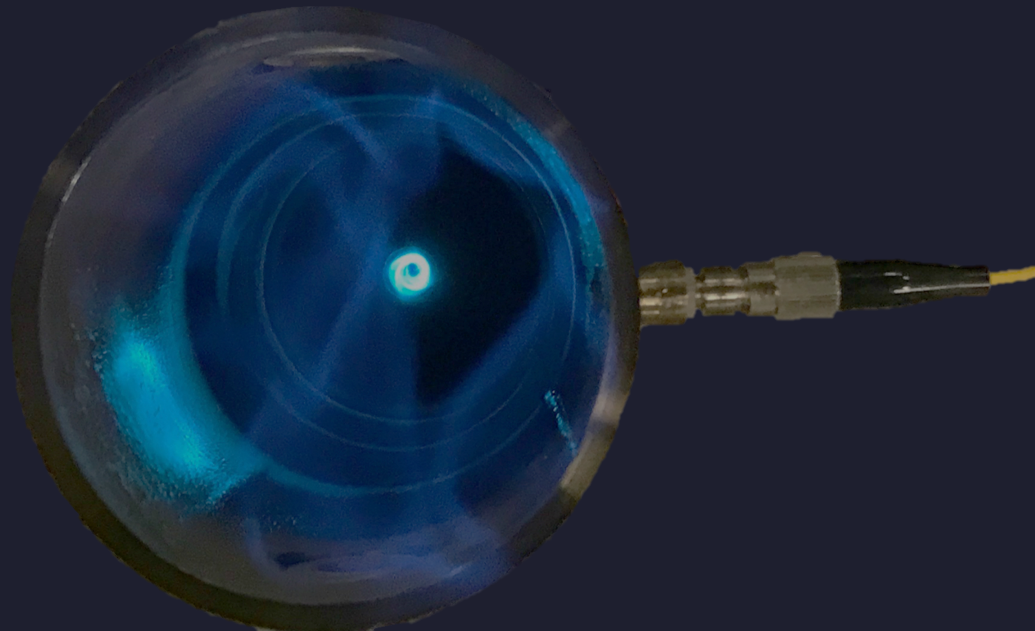
\includegraphics[width=0.55\textwidth]{fig/ch1_fig1.png}
        \caption{Single-ended LAS sensor for temperature and ${H_2}O$ measurements in a propane burner.}
    \label{fig:ch1_1}
\end{figure}

\section{Review of the Literature}
\subsection{Traditional Line-of-Sight Laser-Absorption Sensor}
The use of line-of-sight LAS in combustion is traced back to the late 1970s. In 1977, tunable diode lasers (TDLs) were applied to provide two-color thermometry in flame gases for the first time by Hanson \cite{Hanson19771479}. Since then, line-of-sight LAS sensors have been widely used to acquire path-averaged measurements of gas temperature, pressure, composition and velocity in countless combustion environments \cite{Goldenstein2017, HANSON20111, WOLFRUM19981,Allen1998, WERLE1998197, Lackner2007, Schulz2007, BOLSHOV201545, Eckbreth, Kohse, hanson2016spectroscopy}. 

To mention a few examples, Jatana et al. \cite{Jatana:15, Jatana2} made use of TDLs to achieve line-of-sight measurements of temperature, pressure and water concentration in the intake manifold and exhaust of a diesel engine. Mattison et al. \cite{Mattison2007} developed a wavelength-multiplexed line-of-sight LAS sensor to make crank-angle-resolved measurements of temperature and water concentration in a homogeneous-charge-compression-ignition (HCCI) engine (see Fig.\ \ref{fig:ch1_2}). Fused-silica rings and windows were utilized in the top of the cylinder liner to provide line-of-sight optical access in cylinder. In high-speed combustion flows, Goldenstein et al. \cite{goldenstein2014wavelength,goldenstein2014wavelength2} and Spearrin et al. \cite{spearrin1,spearrin2014quantum} employed mid-infrared LAS sensing of temperature, $H_2O$, $CO_2$ and $CO$ in scramjets and detonation engines \cite{goldenstein2015infrared}. Jackson et al. \cite{Jackson2015} presented a in-flight water-based measurements at the exit of the HIFiRE 2 scramjet combustor (see Fig.\ \ref{fig:ch1_3}). Eight near-infrared (NIR) sensors were used to provide measurements across 5 vertical and 3 horizontal lines of sight. While very useful, these sensors are limited to applications that can provide line-of-sight optical access.

\vspace{5mm}

\begin{figure}[ht]
    \centering
        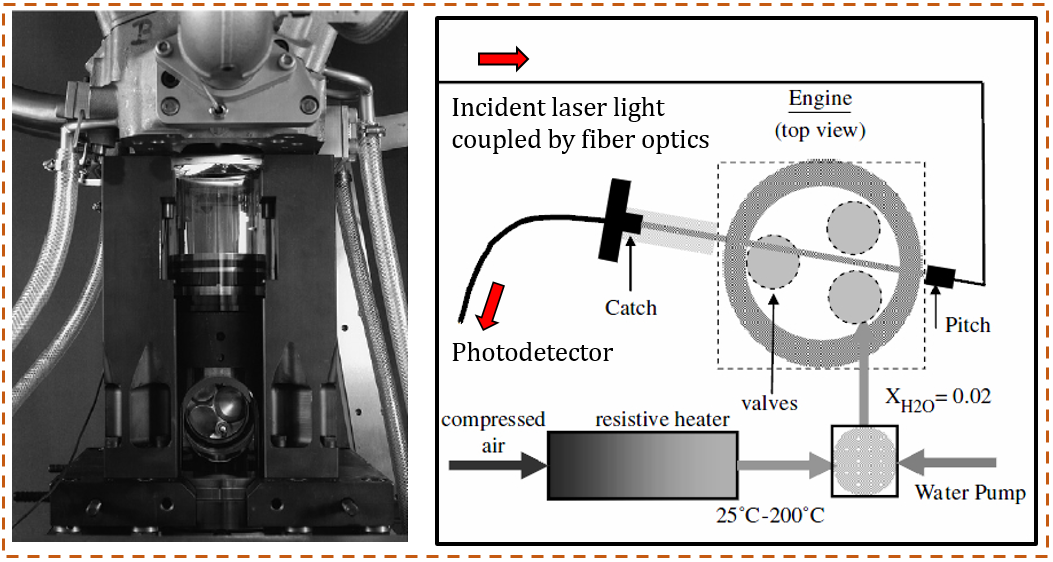
\includegraphics[width=0.75\textwidth]{fig/ch1_fig5.png}
        \caption{Left: an optical HCCI engine at Sandia National Laboratories; Right: a schematic of the fiber-optic-based LOS sensor for the temperature and $H_2O$ measurements in HCCI engine. Figure adapted from Mattison et al. \cite{Mattison2007}.}
    \label{fig:ch1_2}
\end{figure}

\begin{figure}[ht]
    \centering
        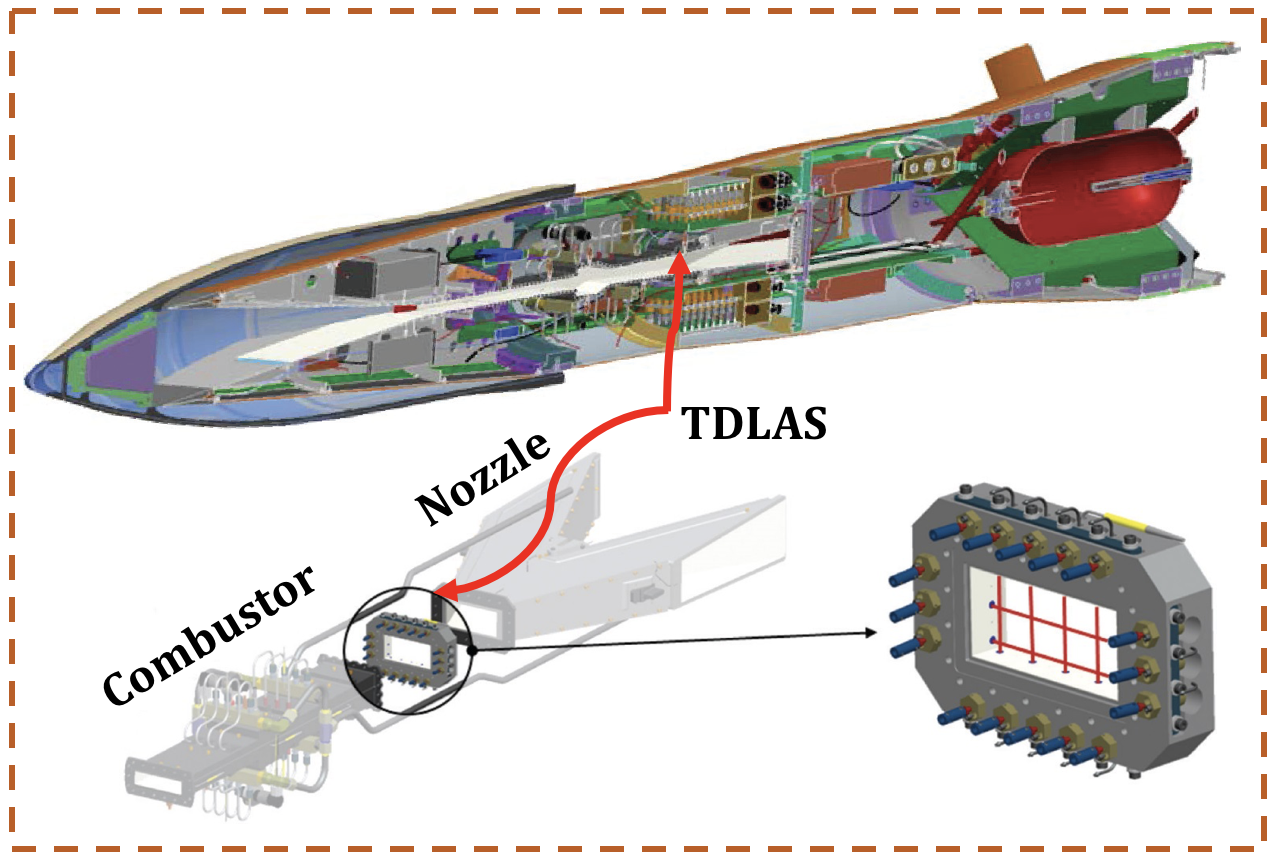
\includegraphics[width=0.7\textwidth]{fig/ch1_fig6_v2.png}
        \caption{Schematic of in-flight TDLAS sensor with 8 lines-of-sight in the HIFiRE 2 scramjet. Figure adapted from Jackson et al. \cite{Jackson2015}.}
    \label{fig:ch1_3}
\end{figure}


\subsection{Single-Ended LAS Probes}
Several researchers have developed single-ended probe-based LAS sensors to study combustion within internal combustion (IC) engines \cite{Melin2017, RIEKER20073041, Jeffries2010, Witzel2013, Bürkle2018}. Rieker et al. \cite{RIEKER20073041} acquired measurements of temperature and $H_2O$ concentration with a spark-plug-embedded probe in IC engines. Measurements were able to be made a temperatures from 500 to 1050 $K$ and pressures from 1 to 50 $atm$ with a bandwidth of 7.5 $kHz$. Rein et al. \cite{Rein:10} developed a Fourier Transform Spectroscopy (FTS) technique to get absorption spectra and measure temperature and water concentration using a optical spark plug probe (OSSP). Fig.\ \ref{fig:ch1_4} illustrates a schematic of a fiber-optic spark plug probe in detail. The incident laser beam passes through a sapphire window into the probe housing, which has channels to let combustion gases pass through. The laser light is transmitted through absorbing gases and reflected by a gold mirror on the probe. The transmitted beam is then collected by a mutlimode fiber which directs the light to a photodetector. This probe penetrates 5.3 $mm$ into the cylinder and provides an optical path length 10.6 $mm$ due to the double pass. Spark plugs with a single-ended probe-based sensor can be customized with the same specifications as industrial-type spark plugs and applied in production engines \cite{Jeffries2010}. Single-ended probe-based sensors enable measurements of gas properties to be acquired in environments with extremely limited optical access. However, the probe surface is known to perturb the local temperature and velocity field due to heat transfer losses and mechanical obstacles. As a result, this approach is somewhat invasive.

\vspace{30mm}

\begin{figure}[ht]
    \centering
        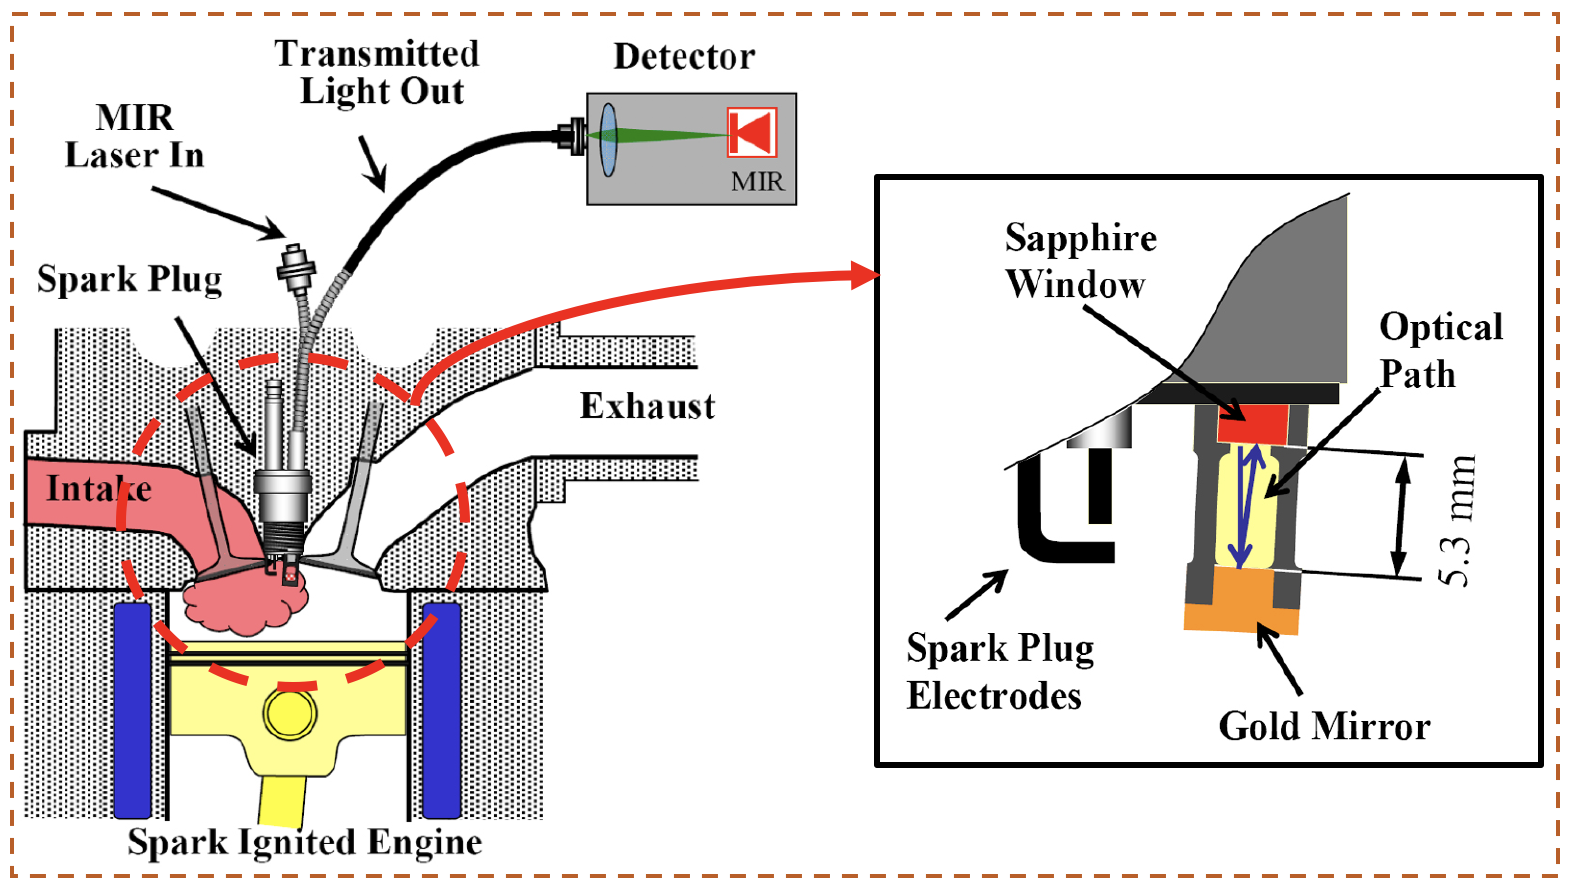
\includegraphics[width=0.7\textwidth]{fig/ch1_fig3.png}
        \caption{Left: A spark-plug optical probe used to provide mid-infrared absorption measurements of temperature and $H_2O$ in cylinder; Right: detailed schematic of the fiber-optic probe. Figure adapted from Jeffries et al. \cite{Jeffries2010}.}
    \label{fig:ch1_4}
\end{figure}

\subsection{Single-Ended, Backscattering-Based LAS Sensors}
Development of single-ended backscattering-based sensors have been a popular area of ongoing research due to their non-intrusive nature and applicability to environments with extremely limited optical access. This type of sensor is capable of standoff or remote measurements by collecting laser light that is backscattered off native surfaces. Recently, Goldenstein et al. \cite{Goldenstein:16} developed a single-ended near-IR TDL sensor for stand-off measurements of gas properties using WMS techniques. In this sensor, a lens and fiber bundle were packed in a lens tube with 25.4 $mm$ diameter. This sensor achieved collection efficiencies from 1 to $10^4$ parts-per-million (ppm) at a stand-off distance between 10 $m$ to 10 $cm$. Melin et al. \cite{Melin2017} made use of a backscattering-based single-ended LAS sensor to acquire water vapor measurements at 10 $kHz$ in a HCCI engine. Most recently, Peng et al.  \cite{Peng:16} demonstrated the first single-ended LAS sensor employing mid-IR wavelengths to provide measurements of $H_2O$, $CO$ and $CO_2$ simultaneously (see Fig.\ \ref{fig:ch1_5}). Later this sensor was used to characterize a rotating detonation engine \cite{Peng2018}.


\begin{figure}[ht]
    \centering
        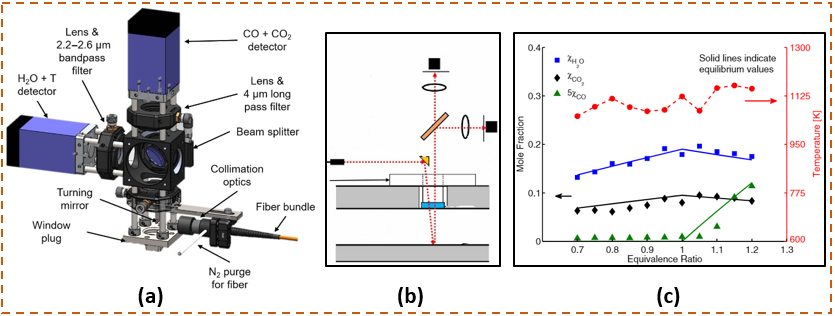
\includegraphics[width=1\textwidth]{fig/ch1_fig4.png}
        \caption{(a) CAD rendering of the single-ended sensor optical architecture; (b) a schematic of the optical path in the single-ended sensor architecture; (c) average temperature and $H_2O$, $CO$ and $CO_2$ mole fractions as a function of equivalence ratio. Figures adapted from Peng et al. \cite{Peng:16}.}
    \label{fig:ch1_5}
\end{figure}

\section{TDLAS of $H_2O$ Transitions in the Near-IR}
The use of LAS sensors relies on spectroscopic knowledge of the selected transitions of the target species. In practical applications, the detection limit of an absorption sensor depends on the transition strength or linestrength of the targeted transitions as this is the primary property that governs the amount of light absorbed by the target species. Water has relatively strong transitions in the near-IR since its vibrations are highly anharmonic which makes it well suited for detection via near-IR TDLs. $H_2O$ is also an attractive combustion species to study since it is a primary combustion product and an indicator of combustion efficiency (especially for $H_2$-fueled combustors). Therefore, $H_2O$ has become one of the most widely used target species in LAS sensors. Fig.\ \ref{fig:ch1_6} illustrates the absorption spectrum of $H_2O$ in the near-IR and mid-IR. Experiments presented in this thesis (Chapter 4) focuses on demonstrations of LAS sensors operated in the near-IR (near 1400 nm). This enabled use of robust telecommunication-grade tunable diode lasers and fiber optics which facilitated the design and fabrication of a new SE-LAS sensor. Further, the wavelength of these TDLs can be tuned by varying the laser current which facilitates the use of scanned-wavelength direct-absorption techniques and wavelength-modulation spectroscopy techniques. 

%As a near-IR hardware, distributed-feedback (DFB) lasers are one of the most applied lasers for LAS sensors. The laser can be tuned by a injection current over some wavelength ranges, which plays an important role in LAS techniques (Chapter 2 and 3). DFB tunable diode lasers (TDL) are capable of their ease if operations, low cost, wavelength stability, and customized tunability over a wide range of wavelengths (760 nm to 3$\mu m$) \cite{Goldenstein2017}.

%\vspace{5mm}

\begin{figure}[ht]
    \centering
        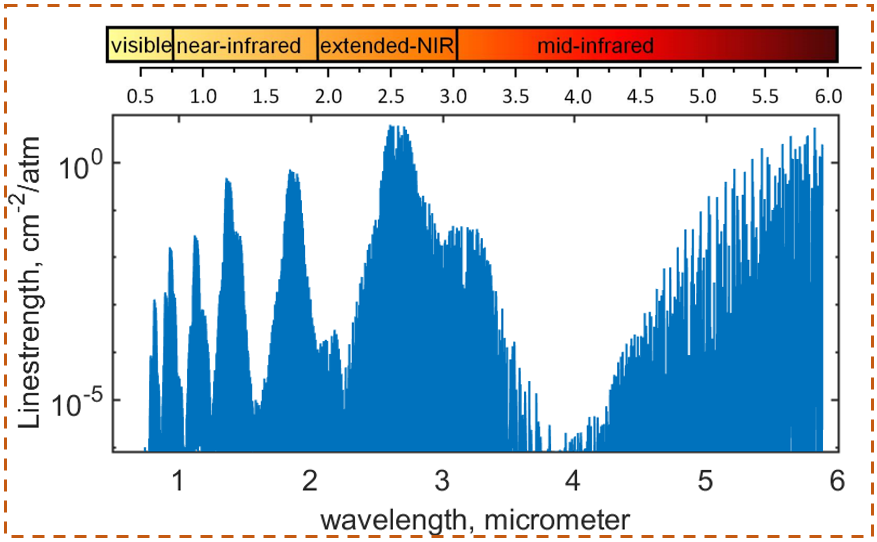
\includegraphics[width=0.7\textwidth]{fig/ch1_fig7.png}
        \caption{Strength of $H_2O$ absorption transitions in the NIR and mid-IR regions. Calculations were performed using the HITRAN 2012 database \cite{2013JQSRT.130....4R}.}
    \label{fig:ch1_6}
\end{figure}

%Applications of three types of LAS sensors: (a) line-of-sight sensor in engine measurements from []; (b) spark-plug-mounted probes from []; (c) mide-IR single-ended backscatter sensor from native surfaces in a combustor from []
\section{Outline of Thesis}
This dissertation is arranged to describe: 1) the fundamentals of absorption spectroscopy and WMS techniques and 2) the design and validation of a novel SE-LAS sensor architecture capable of providing measurements of temperature and $H_2O$ in combustors.

\begin{itemize}
\item \textbf{Chapter 2} presents the fundamental theory of laser-absorption spectroscopy and related techniques including direct absorption and WMS. 
\end{itemize}

\begin{itemize}
\item \textbf{Chapter 3} describes the operating principles of the wavelength-modulation spectroscopy techniques used in the SE-LAS sensor.
\end{itemize}

\begin{itemize}
\item \textbf{Chapter 4} describes the design and application of a SE-LAS sensor for temperature and $H_2O$ measurements. Two experiments were conducted to demonstrate the SE-LAS sensor: (1) fixed-WMS measurements during a transient ignition blast, and (2) scanned-WMS measurements over 30-minute period with the burner operating at quasi-steady-state. Results are compared with those from a line-of-sight sensor to validate the accuracy of the SE-LAS sensor.
\end{itemize}

%\begin{itemize}
%\item \textbf{Chapter 5} demonstrates singled-ended $H_2O$ sensing for temperature and water concentration in the after-treatment of a Cummins exhaust system located in Herrick Laboratories. A scan-WMS measurement is performed between downstream of diesel particulate filter (DPF) and inlet of selective catalytic reduction (SCR). Results are compared with those from a thermocouple and simulation software. Measurements are taken in the condition with and without urea injection respectively.
%\end{itemize}

\begin{itemize}
\item \textbf{Chapter 5} discusses the conclusions resulting from this work and potential future applications of the SE-LAS sensor.
\end{itemize}

\chapter{FUNDAMENTAL THEORY OF ABSORPTION SPECTROSCOPY}
The fundamentals of laser-absorption spectroscopy are described here to provide the reader with sufficient background to understand the operating principles of WMS and the SE-LAS sensor.

\section{Basic Principles of Laser-Absorption}
According to quantum mechanics, molecular energy is quantized and as a result, molecules exist in discrete energy levels for each energy mode (translation, rotation, vibration, electronic). Absorption spectroscopy is associated with the interaction between the electric dipole moment of molecules and external electromagnetic radiation (e.g., from laser light).  Photons can be absorbed or emitted when the laser light (electromagnetic field) is resonant with the oscillating dipole frequency that results from the motion of atoms or electrons. In modern LAS sensors, typically an instantaneously monochromatic laser beam is transmitted through and partially absorbed by a test gas. The frequency of the laser light set to be resonant with certain absorption transitions of the target molecules and the absorption process pumps molecules from a lower-energy state to a higher-energy state (see Fig. 2.1). The Beer-Lambert relation given by Eq. (2.1) describes the absorption of laser light through a homogeneous gas.
\begin{equation}\label{}
I_\nu^t=I_\nu^0exp(-{k_\nu}L)=I_v^0exp[-\alpha(\nu,T,P,\chi_i,L)]
\end{equation}

\begin{figure}[ht]
    \centering
        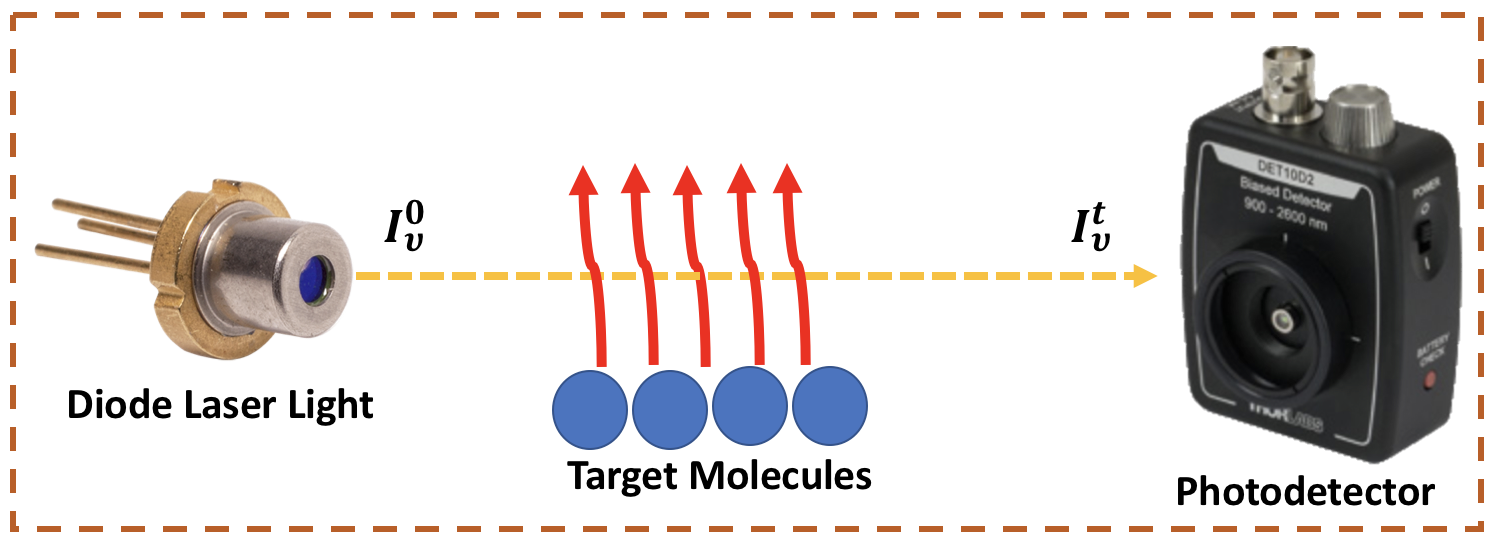
\includegraphics[width=0.7\textwidth]{fig/ch2_fig1_v2.png}
        \caption{Schematic illustrating operating principles of line-of-sight laser-absorption spectroscopy}
    \label{fig:ch2_1}
\end{figure}

\noindent Here, $I_\nu^0$ and $I_\nu^t$ are the incident and transmitted laser-light intensity, $k_\nu$ is the absorption coefficient [$cm^{-1}$], and L is the path length through the absorbing gas [$cm$]. The absorbance, $\alpha$, is defined as the product of $k_\nu$ and $L$. The absorbance is a function of optical frequency $\nu$, temperature $T$, gas pressure $P$, absorbing species mole fraction $\chi_i$ and path length $L$. 

%According to optically thin limit, absorbance $\alpha$ is used to describe the proportion of absorption when $\alpha$ is much less than 1.
%\begin{equation}\label{}
%1-\frac{I_\nu^L}{I_\nu^0}=1-exp(-\alpha)\approx1-(1-\alpha)=\alpha
%\end{equation}

\section{Fundamentals of Absorption Spectroscopy}
\subsection{Absorption coefficient}
The absorption coefficient is given by:
\begin{equation}\label{}
k_v\,[cm^{-1}]=\sum_jS_{i}P\chi_i\phi_j(\nu) 
\end{equation}

\noindent Here, $S_j$ is the linestrength, $\phi_j(\nu)$ is the lineshape function, and the sum over $j$ refers to a sum over all absorption transitions that are significant at frequency $\nu$. The linestrength quantifies the probability of absorption occuring, and the lineshape function is a probability distribution function that describes how the probability of absorption occuring varies with frequency.


%Number density of molecules in state 1 and 2 reach equilibrium when the molecules leaving and entering either state is equal. Proportion of number of molecules in two energy levels can be expressed by Einstein Coefficients: $A_{21}$, $B_{12}$ and $B_{21}$, which describe spontaneous emission, induced absorption and induce emission respectively. This ratio can also be represented by Boltzmann statistical mechanics at equilibrium conditions. Absorption coefficient has the relation given by Eqn.(2.3).

%\begin{equation}\label{}
%k_v[cm^{-1}]=\frac{h\nu}{c}\frac{1}{\delta_{\nu}}[n_2B_{21}-n_1B_{12}]=\frac{h\nu}{c}\frac{1}{\delta_{\nu}}n_1B_{12}(1-exp(-h\nu/kT))
%\end{equation}

%\noindent $h$ is Planck's constant. k is Boltzmann constant. $c$ is light speed. $n_1$ and $n_2$ represent number density of molecules in state 1 and 2. $B_{12}$ stands for probabilities that molecules in state 1 will absorb a quantum and move to state 2 and vice versa for $B_{21}$. In reality, the transition spectra has a certain shape, which is described by normalized lineshape function %$\phi(\nu)$. Therefore,
%\begin{equation}\label{}
%k_v[cm^{-1}]=\frac{h\nu}{c}n_1B_{12}(1-exp(-h\nu/kT))\phi(\nu)
%\end{equation}
%\begin{equation}\label{}
%S_{12}[cm^{-2}]=\frac{h\nu}{c}n_1B_{12}(1-exp(-h\nu/kT))
%\end{equation}
%\begin{equation}\label{}
%k_v[cm^{-1}]=S_{12}[cm^{-2}]\phi(\nu) \quad [cm]
%\end{equation}

%\noindent $S_{12}$ is defined to quantify the absorption transition at frequency $\nu$ and called "line strength". 

\subsection{Linestrength}
In LAS, it is common to define the linestrength in pressure-normalized form [$cm^{-2}atm^{-1}$], however, a per-unit-number-density unit is used in the HITRAN and HITEMP database [$cm^{-1}/(molecule \, cm^{-2})$] \cite{2013JQSRT.130....4R}. Linestrength scales with the number density of molecules in the absorbing quantum state ($n_1$), and the Einstein-B coefficient for stimulated absorption. The number density in the absorbing state can be determined as a function of temperature from Boltzmann statistics and the Einstein-B coefficient can be measured experimentally (using LAS) or taken from spectroscopic databases (e.g. HITRAN). Typically, the linestrength is known at a reference temperature ($T_0$) and then the linestrength at temperature T can be determined from the scaling relation by Eq. (2.3). 

\begin{equation*}
S(T)\,[cm^{-2}atm^{-1}]=S(T_0)\frac{Q(T_0)}{Q(T)}(\frac{T_0}{T})exp[-\frac{hcE^"}{k}(\frac{1}{T}-\frac{1}{T_0})] 
\end{equation*}
\begin{equation}\label{}
\quad[1-exp(\frac{-hcv_{0}}{kT})][1-exp(\frac{-hcv_{0}}{kT_0})]^{-1}  
\end{equation}

\vspace{4mm}

%\begin{equation*}
%S^n(T)=S^n(T_0)\frac{Q(T_0)}{Q(T)}exp[-\frac{hcE^"}{k}(\frac{1}{T}-\frac{1}{T_0})] 
%\end{equation*}
%\begin{equation}\label{}
%\quad[1-exp(\frac{-hcv_{0}}{kT})][1-exp(\frac{-hcv_{0}}{kT_0})]^{-1} \quad [cm^{-1}/(molec \cdot cm^{-2})]
%\end{equation}
\noindent Here, $S(T_0)$ represents the line strength at temperature $T_0 = 296 \,K$, $Q(T)$ is the molecular partition function at temperature $T$, $E^"$ is the lower-state energy, $\nu_0$ is the frequency at the transition line center. Throughout this thesis, the linestrength is calculated using Eq. (2.3) and the absorbance spectrum of $H_2O$ transitions is calculated using Eq. (2.4). An example of simulated absorbance spectra of water transitions near 1.4 $\mu m$ is shown in Fig. 2.2.

%in the demonstration and in the processing of LAS experiment data. By substituting the form of $k_\nu$ into Eqn. 2.6, absorbance at frequency of $\nu$ can be expressed by a relation in Eq.(2.4).
\begin{equation}\label{}
\alpha_\nu=\sum_jS_jP\chi_i\phi_j(\nu)L
\end{equation}

\begin{figure}[ht]
    \centering
        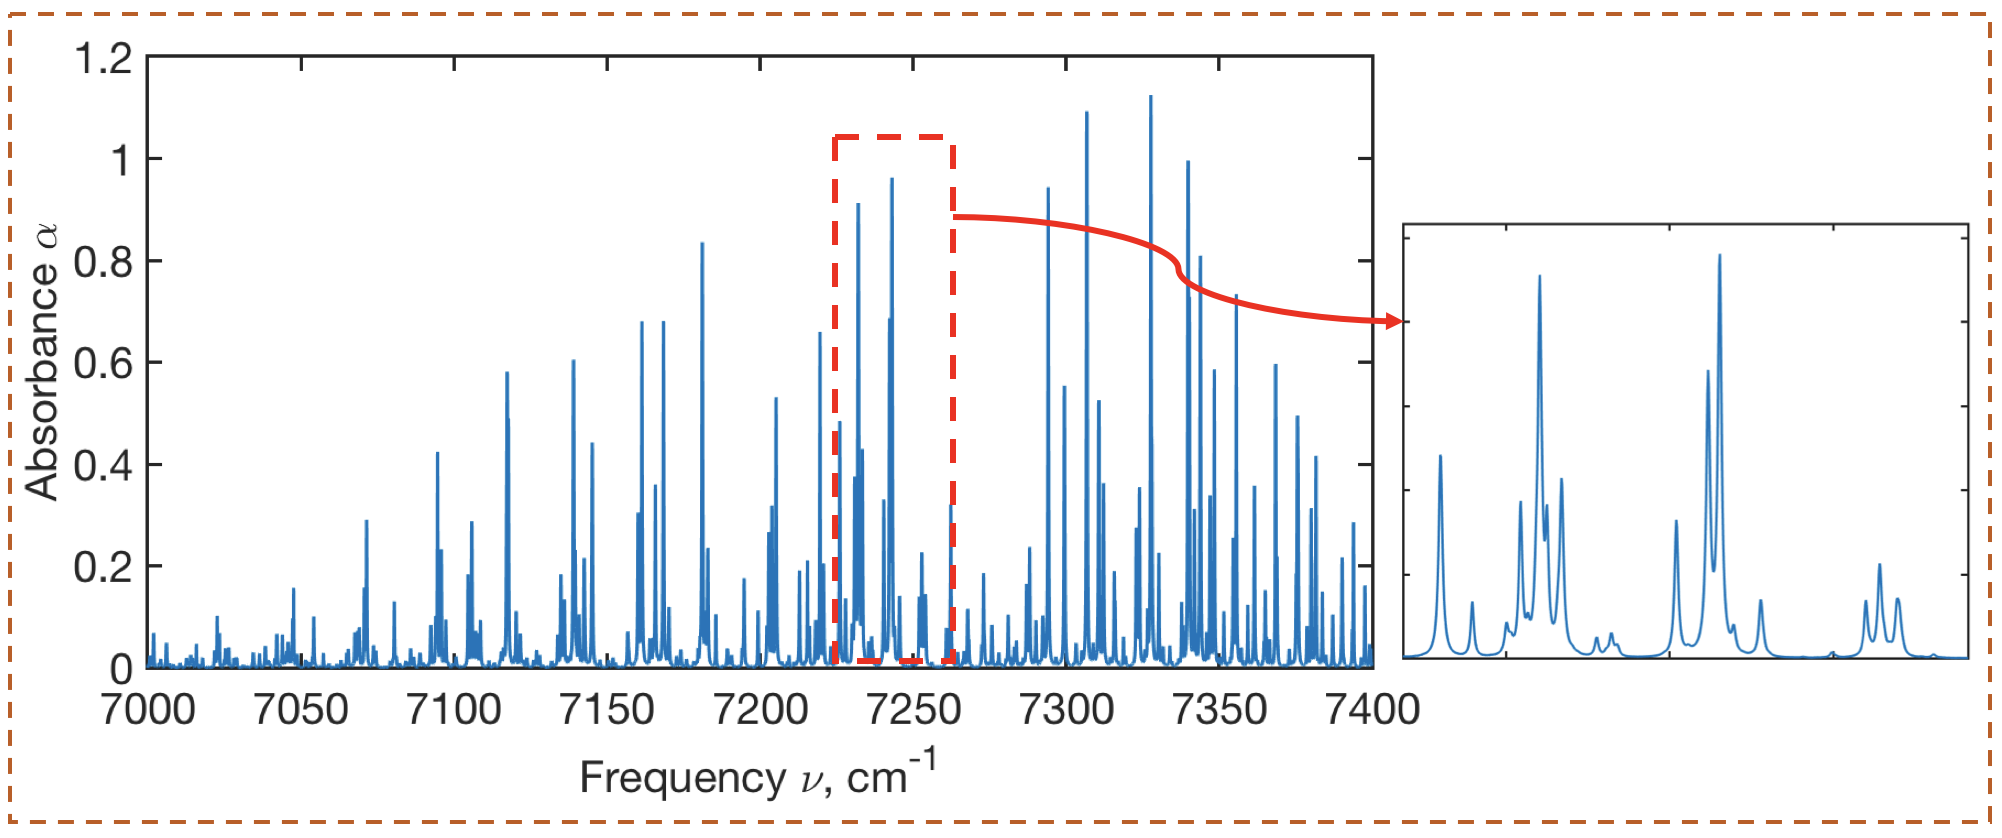
\includegraphics[width=0.85\textwidth]{fig/ch2_fig3.png}
        \caption{Simulated absorbance spectra of $H_2O$ transitions near 1.4 $\mu m$ and a zoom view over a range of 7230 $cm^{-1}$ to 7250 $cm^{-1}$. Calculations were performed for a gas temperature of 300 $K$, pressure of 1 $atm$, $H_2O$ mole fraction of 10$\%$ and path length of 10 $cm$.}
    \label{fig:ch2_2}
\end{figure}

\vspace{50mm}


\subsection{Lineshape function}
While the linestrength describes the ``strength'' or probability of the absorption according due to a given transition, the lineshape function describes how the probability of absorption for a given transition varies as a function of frequency $\nu$. The lineshape function requires knowledge of several line-broadening mechanisms, most importantly, Doppler broadening and collisional broadening.

%absorption coefficient $k_\nu$ is the product of line strength and lineshape function, where line strength describes the absorption quantitatively and line shape indicates the absorption variation as a function of frequency $\nu$. Line shape function is characterized with line broadening mechanisms (mainly Doppler Broadening and Collisional Broadening) and line shift mechanisms (mainly pressure shift). This function has unit-normalized integration across the frequency and is maximized at its line center $\nu_0$.

Doppler Broadening results from a combination of the random thermal motion of the molecules and the Doppler effect. Molecules moving towards the photons see a higher frequency and molecules moving away from the photons see a lower frequency. The random thermal motion of molecules can be modeled using the Maxwellian velocity distribution function and this leads to a Gaussian lineshape. The Doppler full-width at half-maximum (FWHM) is given by Eq. (2.5).

%results from Doppler effects, where the radiation frequency $v_0$ shifts when molecules move in the same direction as the light with different velocities. Because molecules travel in chaos with all directions and different speeds in the space, frequency of molecules detected is closer or far from $v_0$. Statistical molecule velocity is presented in the Maxwellian velocity distribution function. Hence spectra plot as a function of frequency is broadened and the shape of spectra is known as Doppler (a.k.a Gaussian or inhomogeneous) profile. Full width at half maximum (FWHM) is an important parameter in the characterization of spectral lines. Expression of FWHM for Doppler Broadening (Doppler width) is given in Eqn. 2.10.
\begin{equation}\label{}
\Delta\nu_D \,[cm^{-1}]=v_0(\frac{8kTln2}{mc^2})^{1/2}=\nu_{0}*7.1623*10^{-7}*(\frac{T}{MW})^{1/2}
\end{equation}

\vspace{3mm}

\noindent Here, $k$ is Boltzmann constant, $m$ is the particle mass, $c$ is the speed of light, and $MW$ is the molecular weight of the  target molecules in $g$/$mol$. The above equation indicates that the Doppler width is a function of molecular weight, gas temperature and the frequency of the transition. The lineshape profile due to Doppler broadening alone has a Gaussian lineshape function given by Eq. (2.6):

\begin{equation}\label{}
\phi_D(\nu) \,[cm]=\frac{2}{\Delta\nu_D}(\frac{ln2}{\pi})^{1/2}exp\{-4ln2(\frac{\nu-\nu_0}{\Delta\nu_D})^2\}
\end{equation}

\vspace{3mm}

Collisional Broadening, also called pressure broadening, results from a collision-induced uncertainty in the energy of the absorbing state. As molecules travel in the space, inelastic collisions can occur, which reduces the molecule's lifetime in a given quantum state. According to the Heisenberg uncertainty principle, this increased uncertainty in the lifetime of a molecule in a given state leads to a larger uncertainty in the energy of the quantum state. This also leads to molecules to absorb photons over a range of energies/frequencies, and hence broadens the transition lineshape. If the collisional broadening is independent of the molecule's speed, the collisional broadening is homogeneous. The lineshape can be modeled by a Lorentzian function given by Eq. (2.7). 
\begin{equation}\label{}
\phi_L(\nu) \,[cm]=\frac{1}{2\pi}\frac{\Delta\nu_C}{(\nu-\nu_0)^2+(\Delta\nu_C/2)^2}
\end{equation}
%As line width of spectra is determined by molecule lifetime, line shape is thus broadened compared with natural line width. This type of spectra shape is called Lorentzian profile or homogeneous profile. Expression of FWHM for Collisional Broadening is given in Eqn. 2.12.

\vspace{3mm}

\noindent The collisional FWHM ($\Delta\nu_C$) is given by Eq. (2.8).
\begin{equation}\label{}
\Delta\nu_C \,[cm^{-1}]=\sum_A Px_A2\gamma_{B-A} 
\end{equation}

\noindent Here, $B$ is the absorbing molecule, $A$ represents a set of collisional partners of $B$ in the test gas, $P$ is pressure in the unit of $atm$, $x_A$ is mole fraction of species $A$, and $2\gamma_{B-A}$ is the collisional broadening coefficient. The temperature scaling of $\gamma_{B-A}$ can often be modeled using:
\begin{equation}\label{}
\gamma_{B-A}(T)=\gamma_{B-A}(T_0)*(T/T_0)^{n}
\end{equation}

%Broadening coefficient is temperature-dependent because temperature is related to thermal motions of molecules.
\noindent where, $n$ is the temperature scaling exponent which can be found in spectroscopic databases or measured experimentally. Hence collisional width $\nu_C$ is a function of pressure, temperature and properties of collisional partners.

\begin{table}[h]
\begin{center}
\begin{tabular}{ c c c }
\hline
Species & Wavelength $[cm^{-1}]$ & air-broadened coefficient $[cm^{-1}/atm]$\\ \hline
$H_2O$ & 7183.9 & 0.039\\ 
$H_2O$ & 7446.1 & 0.067\\ 
$CO$ & 2059.9 & 0.055\\ \hline
\end{tabular}
\caption{Examples of collisional-broadening coefficient 2$\gamma$ [$cm^{-1}/atm$] in air at 296 $K$. Data taken from the HITRAN 2012 database \cite{2013JQSRT.130....4R}.}
\label{table:ch2_1}
\end{center}
\end{table}

\vspace{-5mm}

Table 2.1 shows some broadening coefficients of $H_2O$ and $CO$ at 296 $K$ and 1 $atm$. These data are taken from the HITRAN 2012 database \cite{2013JQSRT.130....4R}.

%In this thesis, $H_2O$ serves as the target molecule. Accordingly collisional width has a form: 
%\begin{equation}\label{}
%\Delta\nu_C=P*(x*\gamma_{self,T}+(1-x)*\gamma_{air,T})
%\end{equation}
%Where $\gamma_{self}$ and $\gamma_{air}$ are self- and air-broadening coefficients available from HITRAN.

%As mentioned above, collisions between molecules result in intermolecular energy transfer and thus change of their fundamental frequencies for transitions. Because collision width is a function of pressure (Eqn. 2.12), this spectra line shift is known as pressure shift given by Eqn. 2.15. 
%\begin{equation}\label{}
%\Delta\nu_S=\sum_A Px_A\delta_A \quad [cm^{-1}]
%\end{equation}
%\begin{equation}\label{}
%\delta_{T}=\delta_{T_0}*(T/T_0)^{m}
%\end{equation}

%A is a set of collisional partners of target molecule. $\delta_A$ is shift coefficient. Similar as collisional width coefficient, this parameter is also temperature-dependent and the expression is given in Eqn. 2.17. $m$ is temperature coefficient. For $H_2O$ molecule in the air, shifted line center frequency can be written as:
%\begin{equation}\label{}
%\nu_{0,s}=\nu_{0}+\delta_{air}*(T/T_0)^mP(1-x)
%\end{equation}

\subsection{Voigt profile}
At conditions relevant to most combustion gases, Doppler broadening and collisional broadening are both significant. In this case, the Voigt function is typically used to model the lineshape function. The Voigt function is given by a convolution of the Lorentzian and Doppler profiles:

\begin{equation}\label{}
\phi_V(\nu)=\int_{-\infty}^{\infty}\phi_D(u)\phi_L(\nu-u)du=\phi_D(\nu_{0})V(a,w)
\end{equation}

where,

\begin{equation}\label{}
a=\frac{\sqrt[]{ln\,2}\Delta\nu_C}{\Delta\nu_D}
\end{equation}

\begin{equation}\label{}
w=\frac{2\,\sqrt[]{ln\,2}\nu-\nu_{0}}{\Delta\nu_D}
\end{equation}

\begin{equation}
\phi_D(\nu_{0})=\frac{2}{\Delta\nu_D}\,\sqrt[]{\frac{ln\,2}{\pi}}
\end{equation}

\vspace{3mm}

$V(a,w)$ is known as Voigt function, where parameter ``$a$'' illustrates the relative effect on the line profile from collisional and Doppler broadenings, and parameter ``$w$'' is a measure of the distance from linecenter. As shown from Eq. (2.10) to Eq. (2.13), the Voigt profile is a function of linecenter frequency, collisional width and Doppler width. Hence the line shape function can be expressed as:

\begin{center}
$\phi(\nu_{0},\Delta\nu_D,\Delta\nu_C)$
\end{center}

Therefore, the expression of absorbance has the following form:
\begin{equation}\label{}
\alpha(\nu)=\sum_{transitions, j}S_j(T)P\chi_{i,species}\phi_j(\nu_{0,j},\Delta\nu_D,\Delta\nu_C)
\end{equation}

\begin{figure}[b]
    \centering
        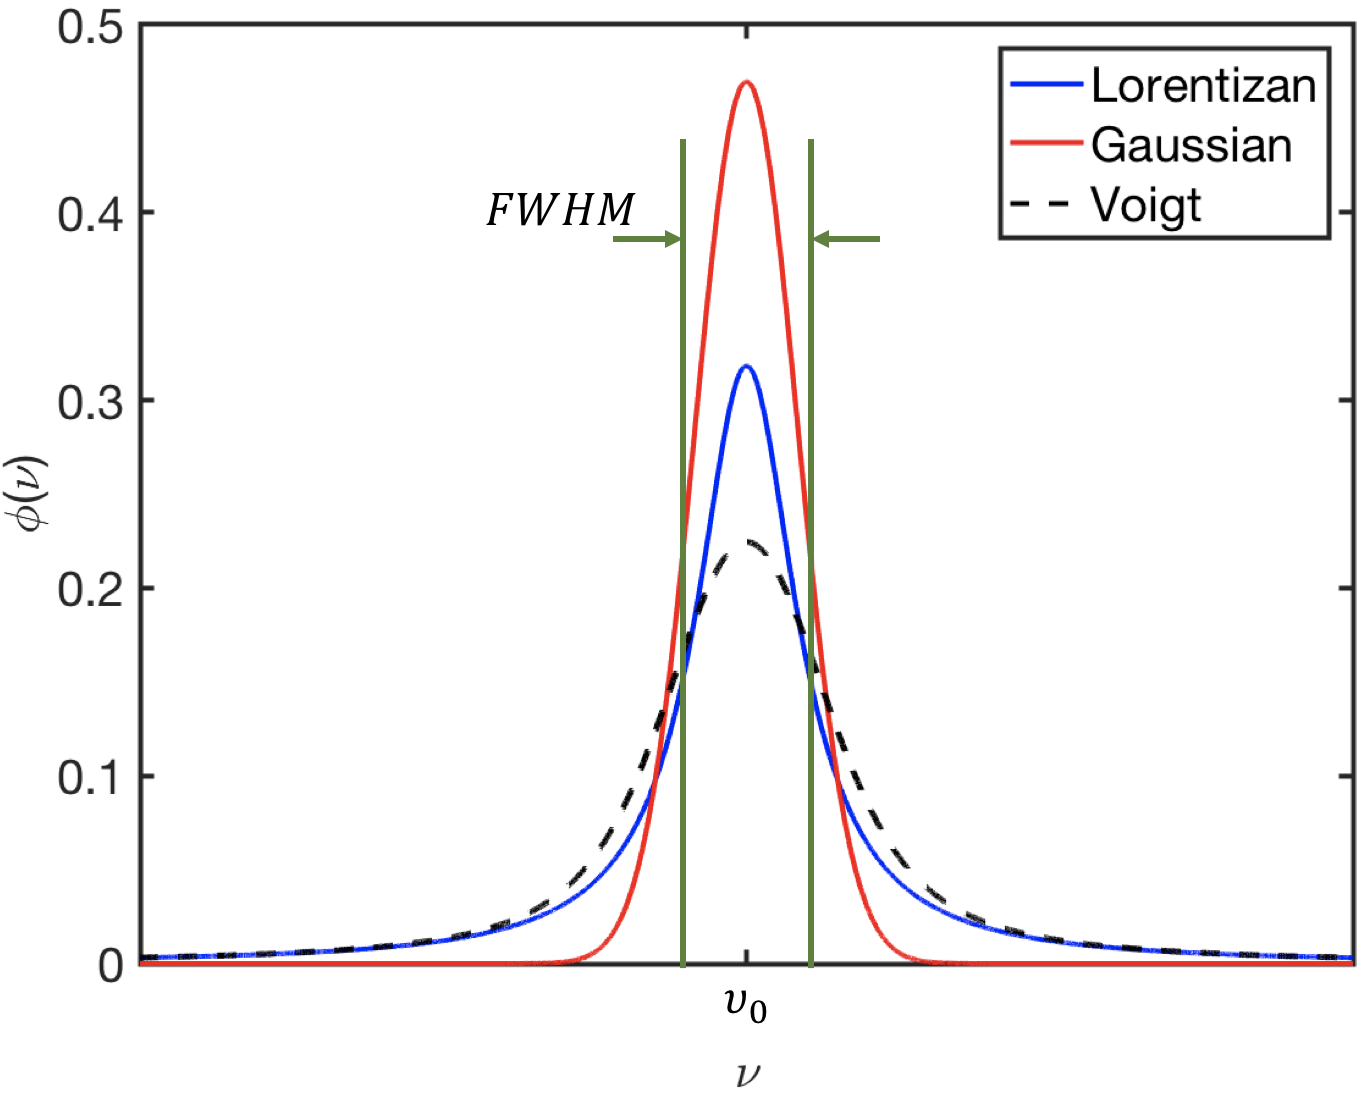
\includegraphics[width=0.6\textwidth]{fig/ch2_fig4.png}
        \caption{Comparison of simulated simulated Lorentzian, Gaussian and Voigt lineshapes with $\Delta\nu_C=\Delta\nu_D$.}
    \label{fig:ch2_3}
\end{figure}

Fig. 2.3 compares Lorentzian (collisional), Gaussian (Doppler) and Voigt lineshapes. In this figure, Lorentzian and Gaussian profiles are simulated with the same FWHM, but the Gaussian profile has a larger peak amplitude and decreases more rapidly away from the linecenter while the Lorentzian profile has larger wings. This indicates that these broadening mechanisms affect the line shape differently and that the Voigt profile is required to account for both of these effects.

%and both are significant for the accuracy of the lineshape simulation. Voigt profile is the combination of the two. It has been widely used with great computational efficiency in multiple applications such as the combustion measurements presented in Chapter 4.

\section{Direct Absorption Techniques}
%Based on Beer's Law (Eqn. 2.1.), this technique is simple but functional. In fixed-wavelength DA, laser beam is transmitted from sources without being scanned (or tuned).
Fixed-wavelength direct absorption (DA) is the simplest laser-absorption diagnostics technique. In this method, the laser light is resonant (at a fixed frequency) with an absorption transition and directed through a test gas onto a detector. Any change in the transmitted light intensity ($I_\nu^t$) is assumed to result from absorption by the target species. As a result, the absorption signal can be detected with a very high bandwidth (MHz), set by the detector bandwidth or sampling rate. For this reason, this technique is frequently used to resolve reaction kinetics in shock tubes \cite{HANSON2014103}. While simple, this technique can suffer from major drawbacks that cannot be easily identified in an experiment. For example, many other factors can decrease or increase the amount of light collected by the photodetector (e.g., beamsteering, background emission), which can lead to large errors in the perceived measurement of absorbance. In addition, the laser frequency may become unstable and lead to errors in interpreting the measured absorbance. 

Scanned-wavelength DA is a more robust technique. By tuning the injection current of a diode laser, the laser frequency can be scanned across an absorption transition to provide a measurement of the absorption spectrum. Laser light then travels through the test gas and gets received by photo-detector. An etalon is used to determine how the wavelength varies in response to current modulation. By taking a ratio of incident and transmitted light intensity, absorbance as a function of wavelength can be obtained. If individual absorption transitions are resolved, the integrated absorbance, $A$, can be obtained which is directly related to linestrength, pressure and path length (Eq. (2.15)) and independent of the transition lineshape. That also indicates that if two laser are applied at the same time, the ratio of integrated absorbance for two lines can be determined which is only a function of temperature (Eq. (2.16)). Hence temperature can be determined from the two-color ratio of integrated absorbance, R, given by Eq. (2.17).
%Absorption signal is able to be detected with high bandwidth at the rate of sampling rate, so fix-wavelength DA can achieve fast measurements and be applied in blast measurements, for example. Drawback of this technique is that laser frequency may become unstable for long-time measurements. Instead, scan-wavelength DA behaves more robust. 
\begin{equation}\label{}
A_{int}=S(T)\times P \times \chi \times L \times \int_{-\infty}^{\infty}\phi(\nu) \cdot dv=S(T) \times \chi \times P \times L
\end{equation}

\vspace{-2mm}

\begin{equation}\label{}
R(T)=\frac{A_1}{A_2}=\frac{S_1(T)}{S_2(T)}
\end{equation}

\vspace{-2mm}

\begin{equation}\label{}
T=\frac{\frac{hc}{k}(E_2^"-E_1^")}{ln\,(A_1/A_2)+ln\,(\frac{S_2(T_0)}{S_1(T_0)})+\frac{hc}{kT_0}(E_2^"-E_1^")}
\end{equation}

\vspace{5mm}

Once the gas temperature is obtained, the absorbing species mole fraction can be calculated from the measured integrated absorbance of either transition (eq. (2.18)).
\begin{equation}\label{}
\chi=\frac{A_{int}}{S(T)PL}
\end{equation}

 \begin{figure}[h]
    \centering
        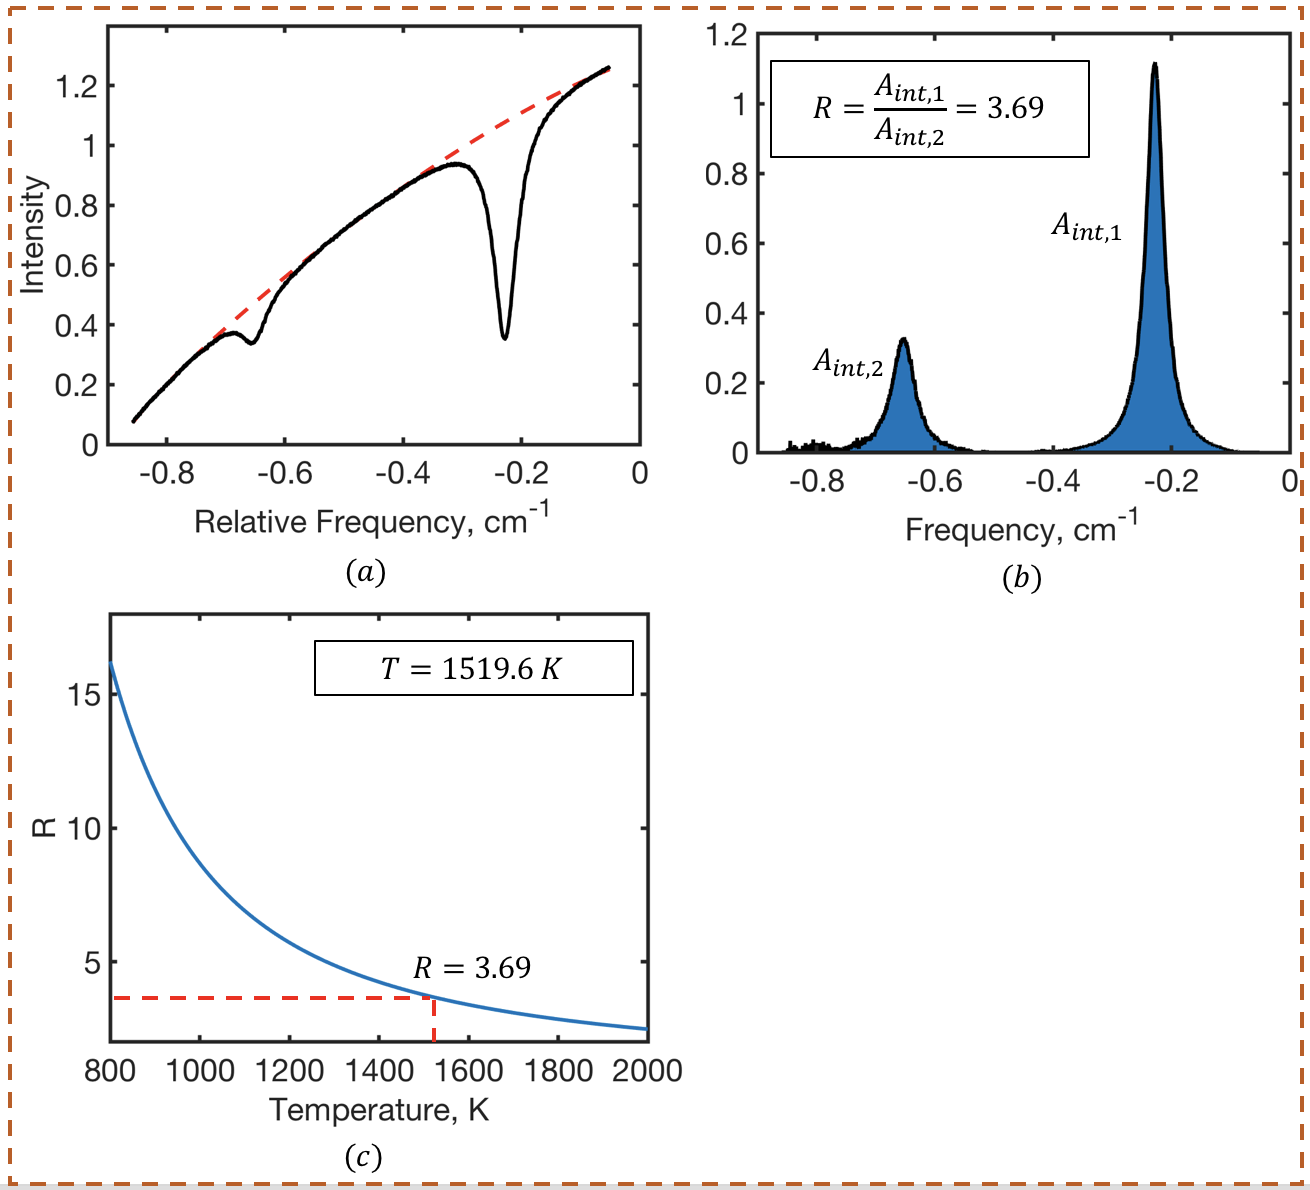
\includegraphics[width=0.7\textwidth]{fig/ch2_fig2_v3.png}
        \caption{Example of Scanned-wavelength DA measurement near 4.85 $\mu m$ for CO and temperature measurements in a $C_2H_4$-$air$ diffusion flame. (a) transmitted signal and baseline-fitted incident intensity; (b) absorbance spectra for both transitions and the two-color ratio of integrated absorbance, $R$; (c) $R$ as a function of temperature.}
    \label{fig:ch2_4}
\end{figure}

Fig. 2.4 illustrates the key steps associated with a scan-DA experiment. The measured light intensity is curve-fitted with $3^{rd}$-order polynomial to non-absorbing regions in order to determine the incident light intensity \textit{in situ}. Beer's Law is then used to calculate the measured absorbance spectrum and Voigt profiles are fit to the measured spectrum to determine the integrated absorbance of each transition (see Fig.2.4 (b)). Temperature can then be inferred using Eq. (2.16) and Eq. (2.17). The above process can be repeated to acquire a time history of temperature in an experiment. 

Scanned-wavelength DA exhibits several significant advantages compared to fixed-wavelength DA. First, the integral of line profile function is unit-normalized, determination of temperature and absorbing species mole fraction does not require knowledge of the lineshape broadening parameters. Second, by performing wavelength and intensity scanning, the incident light intensity can be inferred $in\,situ$ from baseline fitting, thereby accounting for non-absorbing transmission losses. However, scanned-wavelength DA can suffer from low signal-to-noise ratio (SNR) in harsh environments that produce low optical throughputs and strong beamsteering-induced noise. When the transmitted light-intensity is small, electronic noise can cause the SNR for scanned-wavelength DA to be low and fluctuate significantly, and make it difficult to accurately measure small absorbance signals. To overcome these problems, wavelength modulation spectroscopy (WMS) was used, and will be discussed in the next chapter.

%has a drawback about measurement accuracy. Accurate LAS measurements rely on the signal quality from detectors and other electrical instruments. Signal-to-Noise ratio (SNR) is an important indicator to evaluate measurement quality, which is the ratio of mean signal power over standard deviation intensity in the noise. When the signal power is not large, SNR for scan-wavelength DA can fluctuate significantly. That results from (1) baseline fitting and (2) beam steering and scattering. As shown in Fig 2.2, incident intensity is curve-fitted with high-order polynomials based on transmitted intensity. However in some applications, it is difficult to identify and curve-fit signal due to some overlaps between transitions and their neighbors. Another source to affect SNR of DA is beam steering or scattering. That leads to attenuations of detected signals and thus make measurements of transmitted intensity of baseline-fitting of incident intensity inaccurate.


\chapter{WAVELENGTH-MODULATION SPECTROSCOPY TECHNIQUES}

Wavelength modulation spectroscopy (WMS) is a well-known and widely used LAS technique that offers several noise rejection benefits, making it well-suited for hostile environments and applications with small absorbance. In WMS, the laser intensity and wavelength are modulated sinusoidally at frequency $f_m$, using TDLs and other semiconductor lasers (e.g., quantum-cascade lasers). This is achieved via injection-current modulation. The wavelength modulation shifts absorption information to harmonics of the modulation frequency. Because the modulation frequency is usually very high (near $MHz$), absorption information can be isolated from low-frequency noise (e.g., from electronics or environmental factors). Moreover, all harmonics signals are linearly proportional to the DC laser intensity. As a result, the second-harmonic signal (2$f_m$), which is dominated by absorption, can be normalized by the first-harmonic signal (1$f_m$), which is dominated by laser-intensity modulation, to provide WMS-$2f/1f$ signals that are independent of the DC light intensity. This technique has significant advantages in harsh environment, since the WMS-$2f/1f$ signal is insensitive to noise from beam steering, window fouling, etc.  In this chapter, two WMS techniques known as 	``fixed-WMS'' and ``scanned-WMS'' are discussed.

%WMS can achieve gas measurements with relatively low absorbance down to $10^{-5}$.


 \section{Fixed-WMS}
In fixed-WMS, the laser wavelength is sinusoidally modulated while it is centered on an absorption transition linecenter. This leads to a WMS-$2f/1f$ signal that is constant in time (for constant gas conditions), much like a fixed-wavelength direct-absorption measurement. To convert measured WMS-$2f/1f$ signals to measurements of gas properties, a calibration-free WMS model is required to predict how WMS signals vary with gas conditions ($T$,$P$,$\chi$). In this work, fixed-WMS signals were simulated using the calibration-free WMS model developed by Rieker et al. \cite{rieker2009calibration}. 

In this model, the laser wavelength modulation is modeled according to:
\begin{equation}
\nu(t)=\overline{\nu}+a\,cos(wt) \quad [cm^{-1}]
\end{equation}
\begin{equation}
w=2\pi f_m
\end{equation}

\noindent $\overline{\nu}$ is the center frequency, and $a$ is the modulation depth (i.e., amplitude). The laser's incident laser intensity is modeled to $2^{nd}$ order, according to: 
\begin{equation}
I_0(t)=\overline{I_0}(1+\underbrace{i_0\,cos(wt+\psi_1)}_{1f\,term}+\underbrace{i_2\,cos(wt+\psi_2)}_{2f\,term})
\end{equation}

\noindent Here, $\overline{I_0}$ is the average incident intensity, $i_0$ and $i_2$ are linear and nonlinear amplitudes (normalized by $\overline{I_0}$). $\psi_1$ and $\psi_2$ are the phase shifts between intensity modulation and frequency modulation for both intensity modulation terms. The laser intensity modulation is modeled to $2_{nd}$-order to account for the laser's non-linear response to current modulation, which leads to a small but non-zero WMS-$2f$ background signal. Using this approach, the laser background signal is accounted for in the WMS model. All of the aforementioned laser modulation parameters are measured in laboratory experiments and input into the model as discussed by Rieker et al. \cite{rieker2009calibration}.

A transmission coefficient $\tau$ is defined to quantify the fraction of laser light that is absorbed when traveling through the test gas. $\tau$ depends on gas properties and instantaneous laser frequency with the following expression:
\begin{equation}
\tau(\nu(t))=exp\{-\alpha[\nu(t)]\}=exp[-\sum_{j}S_j(T)P\chi L\phi_j(\nu(t))]
\end{equation}

The transmission coefficient $\tau$ can also be expressed as a Fourier series:
\begin{equation}
\tau(\nu(t))=\frac{I_t(\nu(t))}{I_0(\nu(t))}=\sum_{k=0}^{\infty}H_k(\overline{\nu},a)cos(kwt)=H_0+\sum_{k=1}^{\infty}H_k(\overline{\nu},a)cos(kwt)
\end{equation}

\noindent Here Fourier coefficients $H_0$ and $H_k$ are given by:
\begin{equation}
H_0(T,P,\overline{\nu},a)=\frac{1}{2\pi}\int_{-\pi}^{\pi}\exp\{-\sum_j\,S_j(T) \cdot \phi_j(T,P,\chi,\overline{\nu}+a\,cos\theta) \cdot P \cdot \chi \cdot L\}\,d\theta
\end{equation}
\begin{equation}
H_k(T,P,\overline{\nu},a)=\frac{1}{\pi}\int_{-\pi}^{\pi}exp\{-\sum_j\,S_j(T) \cdot \phi_j(T,P,\chi,\overline{\nu}+a\,cos\theta) \cdot P \cdot \chi \cdot L\}cos k\theta d\theta
\end{equation}

Hence the transmitted laser intensity can be modeled using Eq. (3.8). It is noted that $H_0$ term is equivalent to transmission coefficient at center frequency $\overline{\nu}$. $H_k$ terms are related to the $k$th derivative of transmission coefficient function.  
\begin{equation}
I_t(t)=I_0(t)\tau[\nu(t)]=\overline{I_0}(1+i_0\,cos(wt+\psi_1)+i_1\,cos(wt+\psi_2))(H_0+\sum_{k=1}^{\infty}H_k(\overline{\nu},a)cos(kwt))
\end{equation}

In experiments, a lock-in filter or amplifier is used to extract the X and Y components of the WMS-$1f$ and -$2f$ signals from the measured detector signal. This is illustrated by Fig. 3.1. In the calibration-free WMS model, the X and Y components of the $1f$ and $2f$ signal can be calculated from the Fourier coefficients using Eq. (3.9) through Eq. (3.12).
%$nf_m$ ($nth$ harmonics) signals from the detector. After receiving transmitted signals from detector, the signals carry out the fast Fourier transform and then are multiplied by a sinusoidal function at frequency $nf_m$. Corresponding harmonics signals are isolated and simulated as $S=X+iY$, where X component is obtained by multiplication of $cos2\pi nf_mt$ and Y component by multiplication of $sin2\pi nf_mt$ (Fig 3.1).  Simplified forms of X and Y components for $1f$ and $2f$ signals are demonstrated in Eqn 3.9 - Eqn 3.12.

\begin{equation}
X_1f=\frac{G\overline{I_0}}{2}[H_1+i_0(H_0+\frac{H_2}{2})cos\psi_1+\frac{i_2}{2}(H_1+H_3)cos\psi_2]
\end{equation}
\begin{equation}
Y_1f=-\frac{G\overline{I_0}}{2}[i_0(H_0-\frac{H_2}{2})sin\psi_1+\frac{i_2}{2}(H_1-H_3)sin\psi_2]
\end{equation}
\begin{equation}
X_2f=\frac{G\overline{I_0}}{2}[H_2+\frac{i_0}{2}(H_1+H_3)cos\psi_1+i_2(H_0+\frac{H_4}{2})cos\psi_2]
\end{equation}
\begin{equation}
Y_2f=-\frac{G\overline{I_0}}{2}[\frac{i_0}{2}(H_1-H_3)sin\psi_1+i_2(H_0-\frac{H_4}{2})sin\psi_2]
\end{equation}

\noindent Here, $G$ denotes the electro-optical gain of the detection system. This term will be canceled out by performing 1-$f$ normalization. The magnitude of the WMS harmonic signal ($S_{nf}$) is given by Eq. (3.13):
\begin{equation}
S_{nf}=\sqrt[]{X_{nf}^2+Y_{nf}^2}
\end{equation}

 \begin{figure}[h]
    \centering
        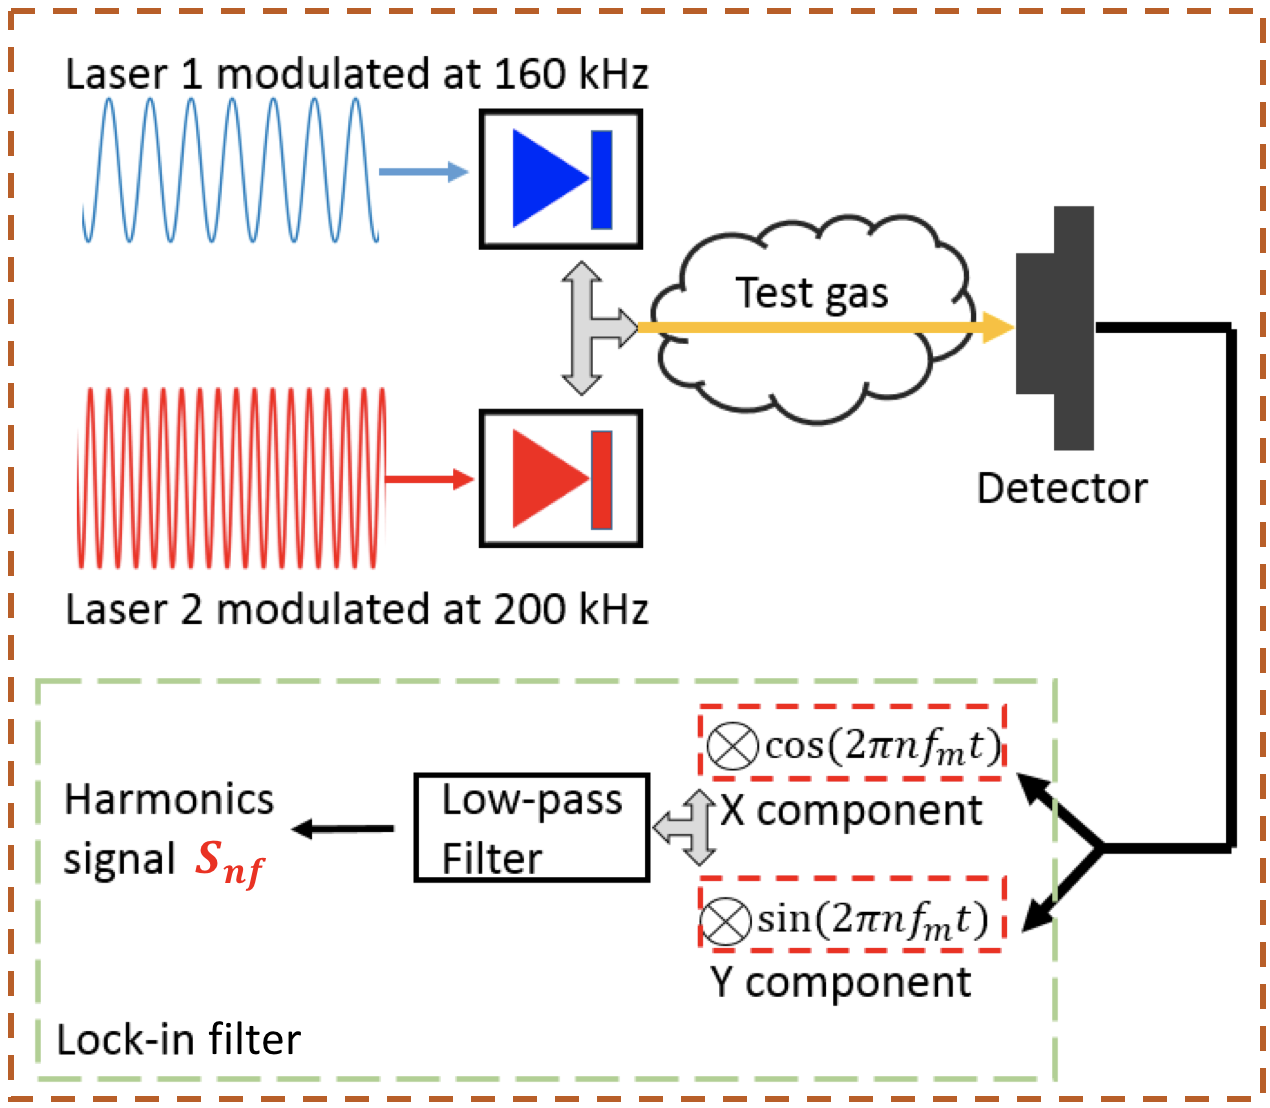
\includegraphics[width=0.85\textwidth]{fig/ch3_fig1_v3.png}
        \caption{Schematic illustrating how WMS harmonic signals are extracted from the detector signal during post-processing.}
    \label{fig:ch3_1}
\end{figure}

As mentioned previously, the WMS-$2f/1f$ signal is immune to variations in DC light intensity (e.g., from beam steering, window fouling, scattering, etc). The absolute value of the WMS-$2f/1f$ signal can be calculated using the calibration-free model according to:
\begin{equation}
S_{2f/1f}=\frac{S_{2f}}{S_{1f}}=\frac{\sqrt[]{X_{2f}^2+Y_{2f}^2}}{\sqrt[]{X_{1f}^2+Y_{1f}^2}}
\end{equation}

It should be noted that $1f$ and $2f$ signals are not zero when the absorption is zero due to the background signals resulting from linear and nonlinear intensity modulation. However, $i_2$ is typically small ($\approx \, \frac{i}{100}i_0$) leading to a near-zero WMS-$2f$ background. When the absorption is zero, the $H_0$ term is equal to 1 and 0 for $H_k$ ($k\neq 0$), which produces the following X and Y components:

\begin{equation}
X_{1f}^0=\frac{\overline{I_0}}{2}i_0cos\psi_1
\end{equation}
\begin{equation}
Y_{1f}^0=-\frac{\overline{I_0}}{2}i_0sin\psi_1
\end{equation}
\begin{equation}
X_{2f}^0=\frac{\overline{I_0}}{2}i_2cos\psi_2
\end{equation}
\begin{equation}
Y_{2f}^0=-\frac{\overline{I_0}}{2}i_2cos\psi_2
\end{equation}

 \begin{figure}[h]
    \centering
        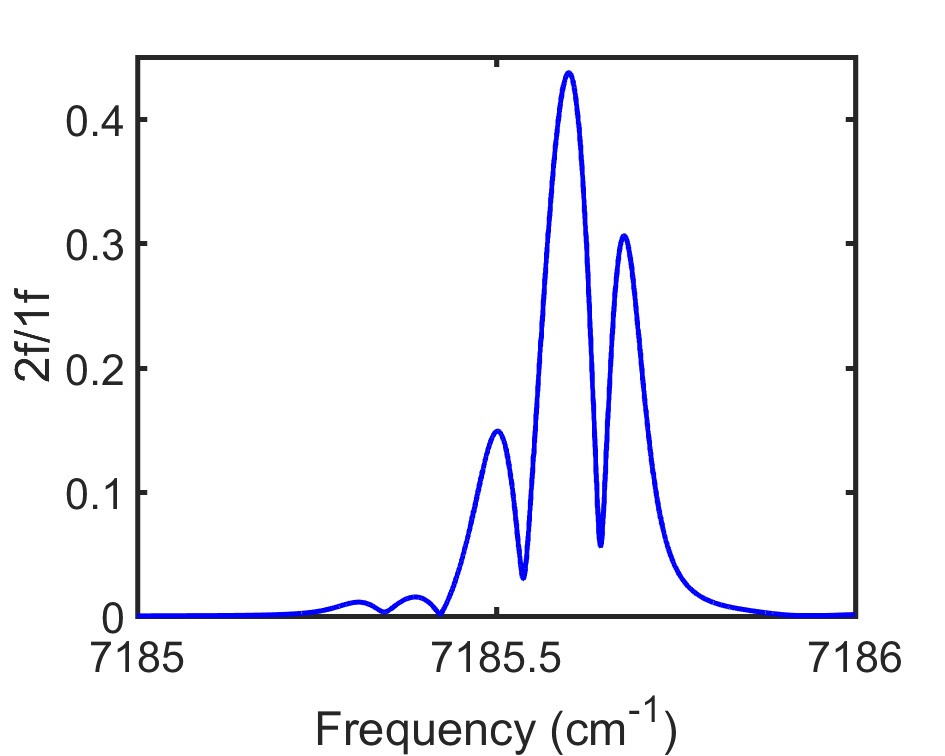
\includegraphics[width=0.7\textwidth]{fig/ch3_fig2.png}
        \caption{Simulated WMS-$2f/1f$ signal for a $H_2O$ absorption transition near 1392 nm. The calibration-free model developed by Rieker et al \cite{rieker2009calibration} was used.}
    \label{fig:ch3_1}
\end{figure}

Thus, the background signals are nonzero under absorption-free conditions. In practical applications, these background signals need to be subtracted using the following expression:
\begin{equation}
S_{2f/1f}=\sqrt[]{\left[\left(\frac{X_{2f}}{S_1f}\right)_{raw}-\left(\frac{X_{2f}}{S_1f}\right)_{bg}\right]^2+\left[\left(\frac{Y_{2f}}{S_1f}\right)_{raw}-\left(\frac{Y_{2f}}{S_1f}\right)_{bg}\right]^2}
\end{equation}

\noindent where the subscripts ``raw'' and ``bg'' refer to signals with absorption and laser background and only laser background, respectively.

\section{Scanned-WMS-$2f/1f$}
In scanned-WMS, the laser wavelength is simultaneously modulated and scanned sinusoidally over the absorption feature to obtain WMS spectra, which can improve measurement accuracy. This is directly analogous to direct-absorption techniques. Scanned-WMS has been applied extensively to provide gas property (e.g. $T$, $P$, $\chi$) measurements in harsh environments \cite{Goldenstein2017,Ma2013,Caswell2013,Stritzke2015,Witzel2013,Whitney2011,Makowiecki2017,Rieker2009b,Li2011}. Among scanned-WMS, ``peak-picking scanned-WMS'' and ``full-spectrum scanned-WMS'' have been used to characterize several combustion applications \cite{WOLFRUM19981,HANSON20111,Goldenstein2017,hanson2016spectroscopy,Schulz2007}. In peak-picking scanned-WMS, the laser wavelength is scanned with a small amplitude to obtain only the peak value of the WMS-$2f/1f$ signal near the transition linecenter. This technique provides a known wavelength reference and therefore improves measurement accuracy compared to fixed-WMS \cite{goldenstein20151}. More recently, Goldenstein et al. \cite{Goldenstein2014} developed a calibration-free scanned-WMS-$2f/1f$ spectral-fitting technique which can be applied to full-spectrum scanned-WMS. This spectral-fitting technique does not need \textit{a priori} knowledge of line-broadening information, thus providing advantages in many practical applications where gas conditions and, thus, collisional broadening, are unknown. This technique was used by the single-ended LAS sensor presented in Chapter 4. 

 \begin{figure}[h]
    \centering
        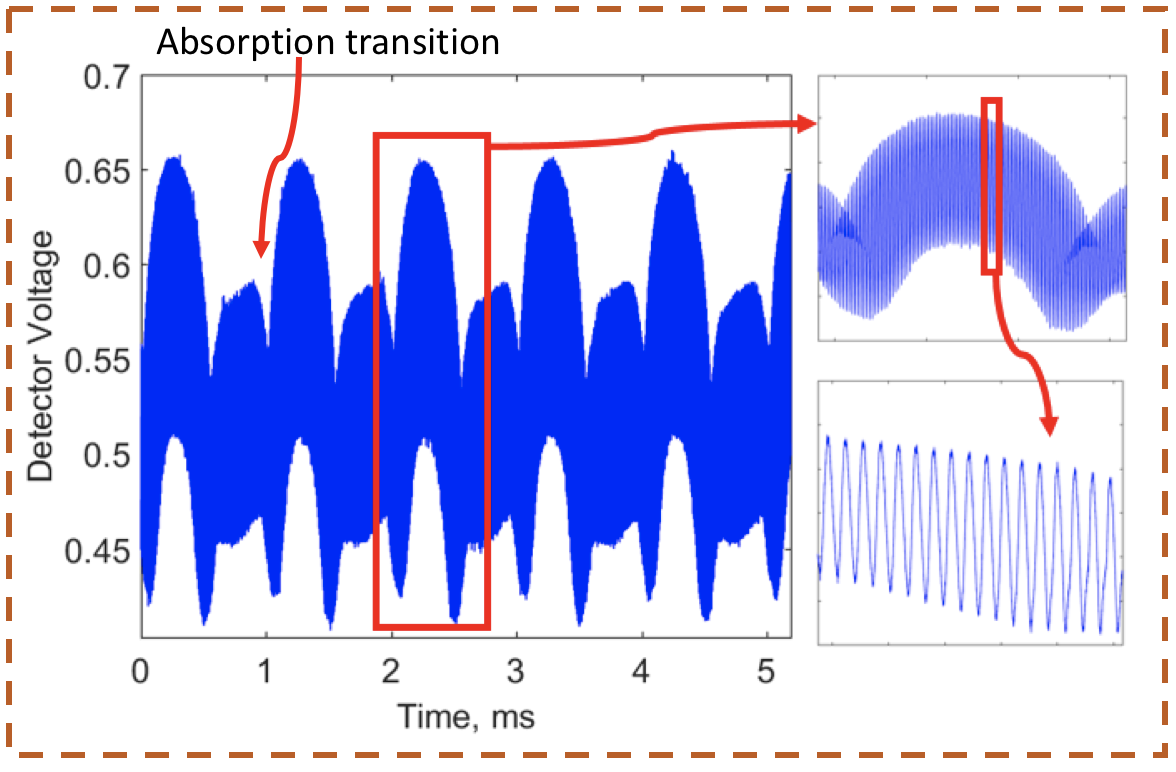
\includegraphics[trim = 0mm 0mm 0mm 0mm, clip=true, width=0.8\textwidth]{fig/ch3_fig3_v2.png}
        \caption{An example of measured detector signal in a scanned-WMS experiment.The laser current is scanned at a frequency of 1 $kHz$ and modulated at a frequency of 160 $kHz$. Subpanels show scan and modulation envelopes in detail.}
    \label{fig:ch4_1}
\end{figure}

Compared to fixed-WMS, in scanned-WMS the incident laser intensity is simulated with an additional sinusoidal signal due to the scan waveform applied to the laser's injection current. In general the scan frequency is $\approx100x$ smaller than the modulation frequency. The incident laser intensity is modeled as:
\begin{equation}
I_0(t)=I_{0,S}(t)+I_{0,M}(t)
\end{equation}

\noindent Here $I_{0,S}$ and $I_{0,M}$ denotes the laser intensity's response to current scanning and modulation respectively. Fig. 3.3 shows an example of the detector signal in a scanned-WMS experiment. The figure shows how the scan and modulation superimpose on each other and how the laser intensity decreases as the laser wavelength is scanned across an absorption transition. The time varying laser frequency can be modeled in a similar manner according to:


\begin{equation}
\nu(t)=\overline{\nu}+\nu_S(t)+\nu_M(t)
\end{equation}
\begin{equation}
\nu_S(t)=a_{1,S}sin(w_St+\psi_{1,S})+a_{2,S}sin(2w_St+\psi_{2,S})
\end{equation}
\begin{equation}
\nu_M(t)=a_{1,M}sin(w_Mt+\psi_{1,M})+a_{2,M}sin(2w_Mt+\psi_{2,M})
\end{equation}

%\vspace{10mm}

\noindent where $\overline{\nu}$ is the line center frequency of the laser. Similar to Eq. (3.3), $a_1$ and $a_2$ represent modulation depths for $1^{st}$ and $2^{nd}$ order, however, it should be noted that $a_{2,S}$ is typically 100$x$ smaller than $a_{1,S}$ and can be ignored in most cases. $\psi_1$ and $\psi_2$ are the phase shift between wavelength and intensity modulation for $1^{st}$ and $2^{nd}$ order terms respectively. After simulating $I_0(t)$ and $\nu(t)$, the time-varying transmitted intensity $I_t(t)$ can be determined using the Beer Lambert relation.
\begin{equation}
I_t(t)=I_0(t)exp[-\phi(\nu(t),T,P,\chi)A]
\end{equation}
Here $A$ represents the integrated absorbance given by:
\begin{equation}
A=\int_{-\infty}^{\infty}\alpha(\nu) d\nu=S(T)P\chi_iL
\end{equation}

 \begin{figure}[h]
    \centering
        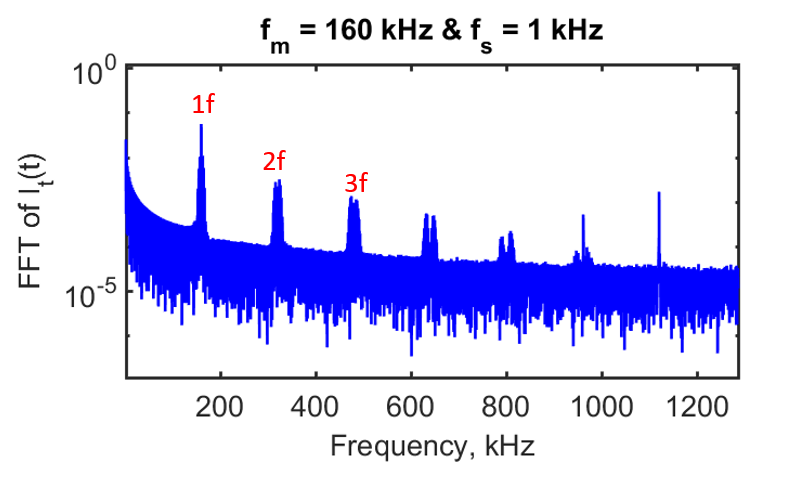
\includegraphics[trim = 0mm 0mm 0mm 0mm, clip=true, width=0.9\textwidth]{fig/ch3_fig5.png}
        \caption{FFT of a measured detector signal for a scanned-WMS-$2f/1f$ experiment. The laser is sinusoidally modulated at the frequency of 160 kHz and scanned at the frequency of 1 kHz. The first three harmonic signals are marked in the picture where $1f$ = 160 kHz, $2f$ = 320 kHz and $3f$ = 480 kHz. The scan waveform introduces sidebands centered around each harmonic.}
    \label{fig:ch3_4}
\end{figure}

After calculating $I_t$, the simulated scanned-WMS-$2f/1f$ signal can be extracted from $I_t$ using a digital lock-in filter. Fig. 3.4 shows a the frequency spectrum of a measured detector signals. The X and Y components of the first two harmonic signals can be isolated and extracted with digital lock-in filters. The magnitude of the WMS-$2f/1f$ signal can then be calculated using Eq. (3.26):

\begin{equation}
S_{2f/1f}=\frac{\sqrt[]{X_{2f}^2+Y_{2f}^2}}{\sqrt[]{X_{1f}^2+Y_{1f}^2}}=f(laser\,parameters,A,\Delta\nu_C,\Delta\nu_D,\nu_0)
\end{equation}

\vspace{3mm}
\noindent which shows that $S_{2f/1f}$ is a function if laser parameters and spectroscopy quantities.

 \begin{figure}[h]
    \centering
        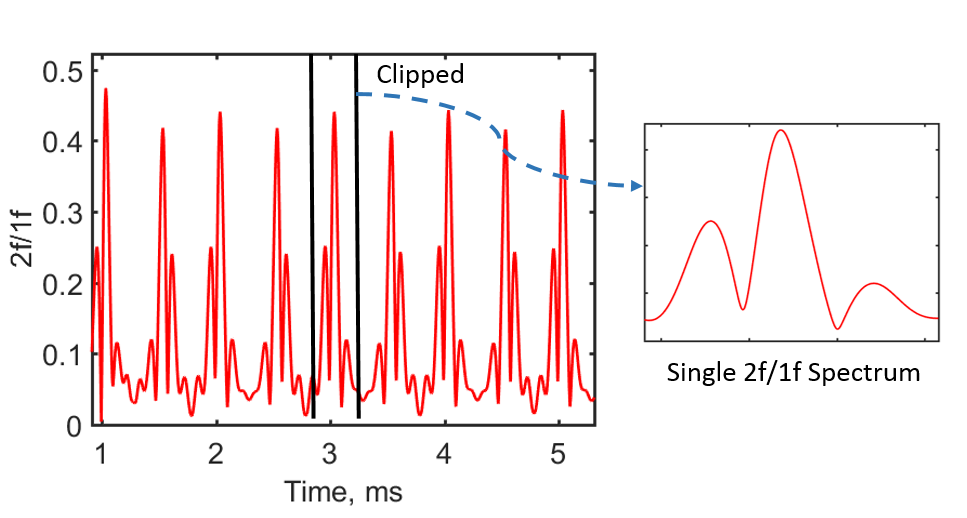
\includegraphics[trim = 0mm 0mm 0mm 0mm, clip=true, width=0.8\textwidth]{fig/ch3_fig6.png}
        \caption{Left: WMS-$2f/1f$ signal time history for a scanned-WMS experiment. The laser is modulated at 160 kHz and scanned at 1000 Hz. It is noted that WMS-$2f/1f$ signals are slightly different for up-scan and down-scan due to the phase-shift between the laser intensity and wavelength. Right: Clipped single spectrum. Spectral fitting is applied to each single spectrum to infer gas properties.}
    \label{fig:ch3_5}
\end{figure}

 \begin{figure}[h]
    \centering
        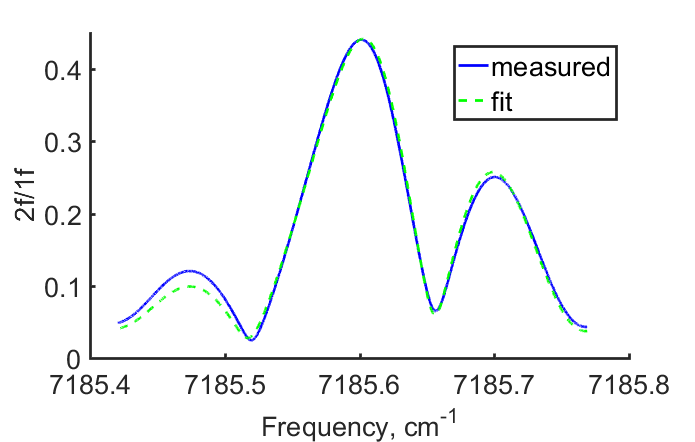
\includegraphics[width=0.7\textwidth]{fig/ch3_fig7.png}
        \caption{An example of a single scanned-WMS-$2f/1f$ spectrum and its best fit. The fitting has a peak-normalized residual less than 4$\%$.}
    \label{fig:ch3_6}
\end{figure}

\vspace{30mm}


Fig. 3.5 illustrates an example of a measured scanned-WMS-$2f/1f$ signal time history. A single spectrum (for an up-scan or down-scan) can then be extracted from the time history and fed to a WMS-$2f/1f$ spectral fitting routine. Here, the spectral-fitting technique developed by Goldenstein et al. \cite{Goldenstein2017} was used in a non-linear least-squares fitting routine to determine the best-fit spectrum and spectroscopic quantities. In this technique, the aforementioned scanned-WMS simulation technique is incorporated into a non-linear least-squares fitting routine. The laser modulation parameters (determined from controlled laboratory experiments), and the Doppler width ($\Delta\nu_D$) are fixed, and $\nu_0$, $A$, and $\Delta\nu_C$ are free-parameters that manipulate the simulated WMS-$2f/1f$ spectrum. Fig. 3.6 shows an example of a measured WMS-$2f/1f$ spectrum and its best fit for an $H_2O$ absorption transition near 7185.6 $cm^{-1}$. The value of $A$ corresponding to the best-fit spectrum is used to determine the absorbing species mole fraction and/or gas temperature analogous to scanned-wavelength direct absorption.


%\section{Characterization of Diode Lasers}


\chapter{DESIGN AND VALIDATION OF SINGLE-ENDED Temperature and \ce{H2O} SENSOR }

\vspace{3mm}

\textit{Parts of this chapter is currently under review as Yuzhe Zhou, Garrett C. Mattews and Christopher S. Goldenstein, ``A compact, fiber-coupled, single-ended laser-absorption-spectroscopy sensor for high-temperature environments,'' Applied Optics (2018).}

\section{Introduction}
TDLAS sensors have been extensively used to acquire non-intrusive, in situ measurements of gas temperature, pressure and composition in many practical combustion environments and energy systems \cite{Goldenstein2017, Ma2013, Caswell2013,Stritzke2015,Bürkle2018, Witzel2013,Makowiecki2017,rieker2009calibration,Li2011}. Typically, traditional laser-absorption sensors, known as LOS-LAS sensors, rely on transmitting laser light across an unobstructed line-of-sight, however this approach is not suitable for some environments with extremely limited optical access or in situations where standoff detection is needed. To overcome this challenge single-ended laser-absorption-spectroscopy (SE-LAS) sensors have been developed, which rely on backscattering laser light off native surfaces \cite{Dubinsky1998,Wainner2002,Wang2015,Goldenstein:16,Peng:16,Peng2018} or surfaces within optical probes \cite{RIEKER20073041,Rein:10,Chen2010,0957-0233-25-11-115501,GIRARD2017158}. Recently, SE-LAS sensors have emerged as a promising approach to characterizing combustion environments with limited optical access \cite{Goldenstein2017}. While promising, all prior single-ended LAS sensing in combustors relied on the use of windows to isolate the SE-LAS sensor from the high-temperature combustion gases. This increases sensor cost and complicates sensor installation since care must be taken during alignment to avoid collecting strong reflections off the window surface which can significantly compromise the accuracy of single-ended LAS sensors.

The design and validation of a compact single-ended laser-absorption-spectroscopy (SE-LAS) sensor for measuring temperature and $H_2O$ in high-temperature combustion gases ($\approx 1000\,K$) is presented in this thesis. The design presented here builds on the fiber-coupled SE-LAS sensor developed previously by Goldenstein et al. \cite{Goldenstein:16} to provide several design improvements which increase the practicality and applicability of laser-absorption sensors without compromising measurement quality. 1) The sensor presented in this thesis is a windowless (in addition to a lens) single-ended LAS sensor which can withstand direct exposure to high-temperature combustion gases. 2) The SE-LAS sensor presented in this thesis use a 18$x$ smaller lens to provide a 9$x$ smaller footprint (compared to \cite{Goldenstein:16}) which enables this sensor to be integrated into environments with tighter spatial constraints. 3) A simple approach for reducing the computational time required to perform scanned-WMS spectral-fitting by a factor of 100 is presented. This enables large datasets to be processed in a reasonable amount of time using personal computers and could facilitate the integration of scanned-WMS-2f/1f techniques into stand-alone sensors.

In this chapter, the architecture of this sensor is demonstrated including experimental setup and sensor housing design first. Then the diagnostics techniques are described with an accelerated scanned-WMS-$2f/1f$ spectral-fitting routine first applied. This section is followed by the demonstration and evaluation of SE-LAS sensor's performance in a propane-air burner including: i) collection efficiency of SE-LAS sensor, ii) comparison of the SE-LAS sensor measurement with that of a traditional LOS sensor and iii) uncertainty analysis of the measurements.

\section{Diagnostic Techniques}
The sensor presented here is demonstrated using first-harmonic-normalized wavelength-modulation spectroscopy with second-harmonic detection (WMS-$2f/1f$) techniques. WMS-$2f/1f$ techniques where the nominal wavelength is fixed (fixed-WMS-$2f/1f$) or scanned (scanned-WMS-$2f/1f$) in time were both used. The former was used to provide measurements with greater bandwidth to resolve an ignition event, while the latter was used to provide greater measurement accuracy via spectral-fitting techniques that avoid the need for knowledge of collisional-broadening coefficients \cite{Goldenstein2014}. These methods and their relative attributes have been described in the previous chapters.

\subsection{Line selection}
Water has been a popular monitoring species in TDLAS for combustion diagnostics \cite{Goldenstein2017}. Accuracy of TDLAS relies on the appropriate line selection, the rules of which have been developed for measuring uniform gas in low-pressure applications \cite{Zhou2005}. Generally the criterion for the line selection includes the linestrength, temperature sensitivity and isolation from neighboring transitions. Strong transitions can give a large gain in detector signals and thus great precision with low SNR. The temperature sensitivity depends on the difference of lower-state energy between two selected transitions, which is give by Eq. (4.1). This work employs near-infrared wavelengths near 1343 nm and 1392 nm to investigate the combination and overtone absorption bands of $H_2O$ utilizing robust semiconductor lasers and telecommunication-grade fiber optics \cite{FURLONG1998103}. These wavelengths were used to interrogate two strong and well-characterized $H_2O$ doublet transitions due to their large strength, isolation from interfering transitions, and disparate lower-state energies (see Table.4.1), the latter of which enables sensitive thermometry at the temperatures of interest here. These wavelengths have been used extensively to characterize combustion environments via TDLAS and some prior works \cite{Goldenstein:16,Goldenstein2014,rieker2009calibration,strand2015quantification} are recommended for greater detail regarding the suitability and performance of LAS sensors employing these wavelengths in combustion systems.

%($\nu_1+\nu_3$ band) ($2\nu_1$, $\nu_1+\nu_3$ band)

\begin{equation}
|\frac{dR/R}{dT/T}|=(\frac{hc}{k})\frac{|E_1^"-E_2^"|}{T}
\end{equation}

\begin{table}[h]
\begin{center}
\begin{tabular}{ c c c c }
\hline
Species & $\nu_0$ $[cm^{-1}]$ & $S(296 K)$ $[cm^{-2}/atm^{-1}]$ & $E^"$ [$cm^{-1}$]\\ \hline
$H_2O$ & 7185.59 & 0.0196 & 1045\\ 
$H_2O$ & 7446.35/.37 & 0.0011 & 1774/1806\\ \hline
\end{tabular}
\caption{Wavelength, linestrength and lower-state energy of the two color transitions used in this work \cite{Goldenstein:16}}
\label{table:ch4_1}
\end{center}
\end{table}


\subsection{WMS-$2f/1f$ model and simulation techniques}
A model capable of predicting WMS-2f/1f signals as a function of gas temperature, pressure, and composition is required to convert measured WMS signals to measurements of gas conditions. These models consist of sub-models for: 1) the absorbance spectrum of the target species and 2) each laser’s wavelength and intensity modulation.
Absorbance spectra of the selected transitions were calculated using the algorithms presented in \cite{GOLDENSTEIN2017249}. Simulations were performed using the HITRAN2012 database \cite{2013JQSRT.130....4R} in combination with the experimentally validated linestrength and collisional-broadening parameters. Fig. 4.1 shows simulated absorbance spectra for the relevant wavelength region at conditions representative of the propane-air burner operating at quasi-steady state (1000 $K$, 1 $atm$, $10\%$ $H_2O$ by mole). 

For simplicity, fixed-WMS-2f/1f signals were simulated using the calibration-free WMS model developed by Rieker et al. \cite{rieker2009calibration}. This model requires knowledge of the wavelength-modulation depth ($a_m$), $1^{st}$ and $2^{nd}$-order intensity modulation amplitudes ($i_0$, $i_2$), and the phase shift between wavelength and intensity modulation ($\psi_1$, $\psi_2$). The laser-modulation parameters were determined according to the methods described in \cite{rieker2009calibration}.

Typically, this simulation technique has been directly integrated in a least-squares fitting routine with the integrated absorbance ($A$), collisional width ($\Delta\nu_C$), and transition linecenter frequency ($\nu_0$) as free parameters \cite{Goldenstein:16,Goldenstein2014,goldenstein2014scanned,spearrin2014simultaneous}. The parameters corresponding to the best-fit spectrum are then used to calculate gas properties. While accurate, this approach is computationally expensive, typically requiring 10$s$ of seconds (using MATLAB's function $nlinfit$ on a modern personal computer) to find the best-fit scanned-WMS-$2f/1f$ spectrum for a single measurement. The following subsection presents a simple solution to reducing computational time by using a pre-calculated library of scanned WMS-$2f/1f$ spectra.

\begin{figure}  
\begin{minipage}[h]{0.5\linewidth}  
\centering  
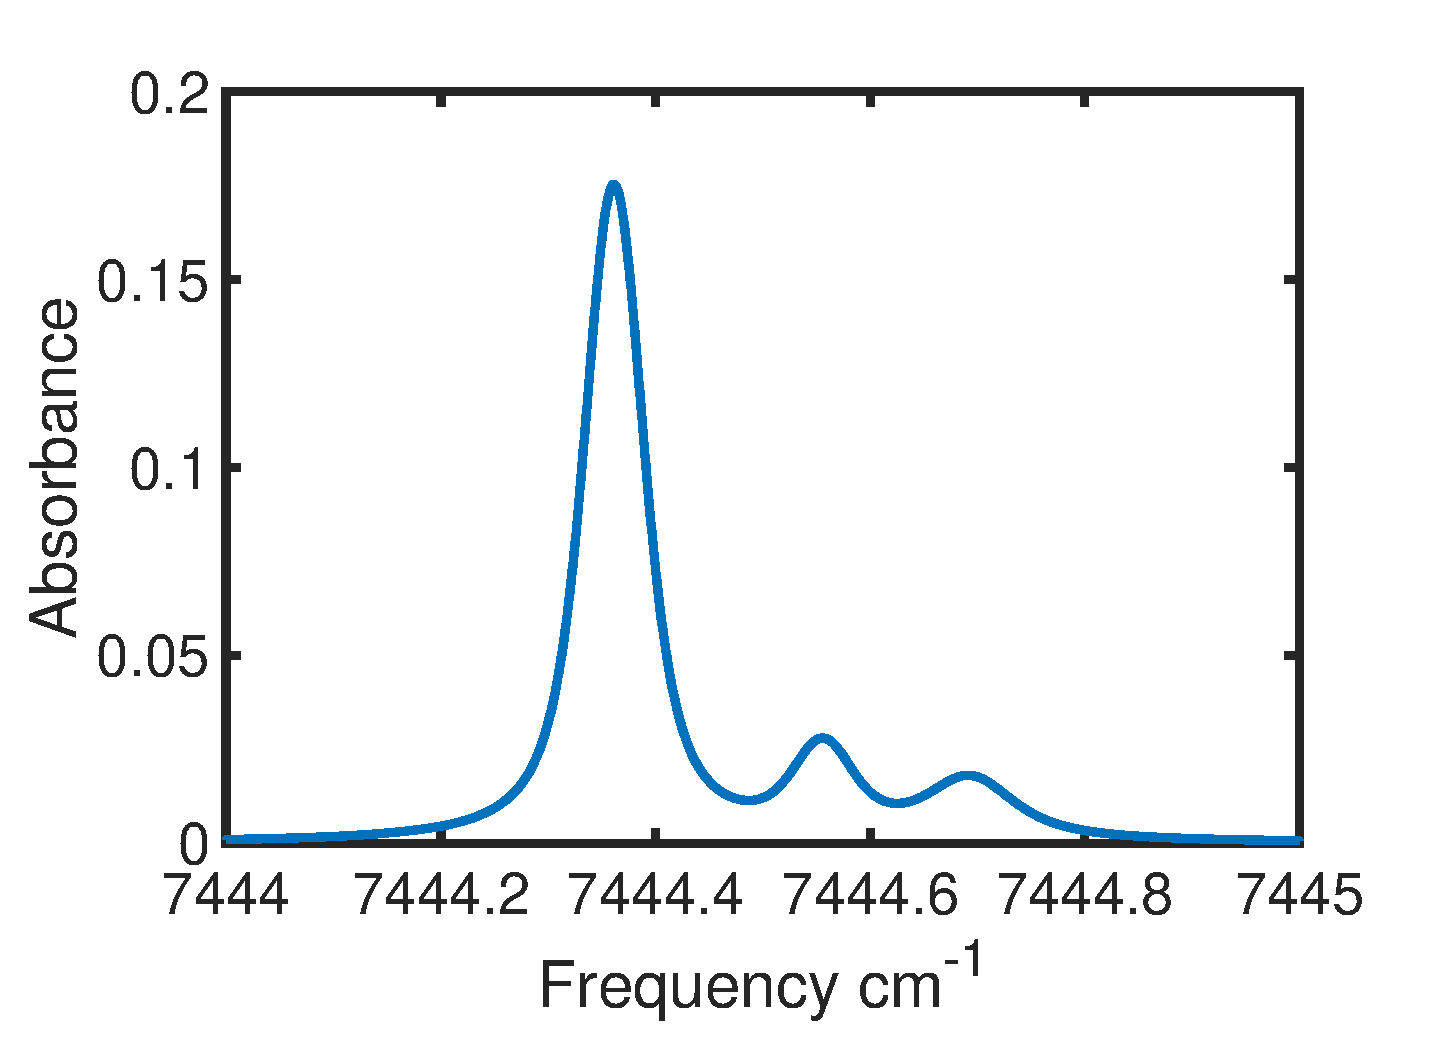
\includegraphics[width=1\textwidth]{fig/ch4_fig3_1.eps}  
\end{minipage}%  
\begin{minipage}[h]{0.5\linewidth}  
\centering  
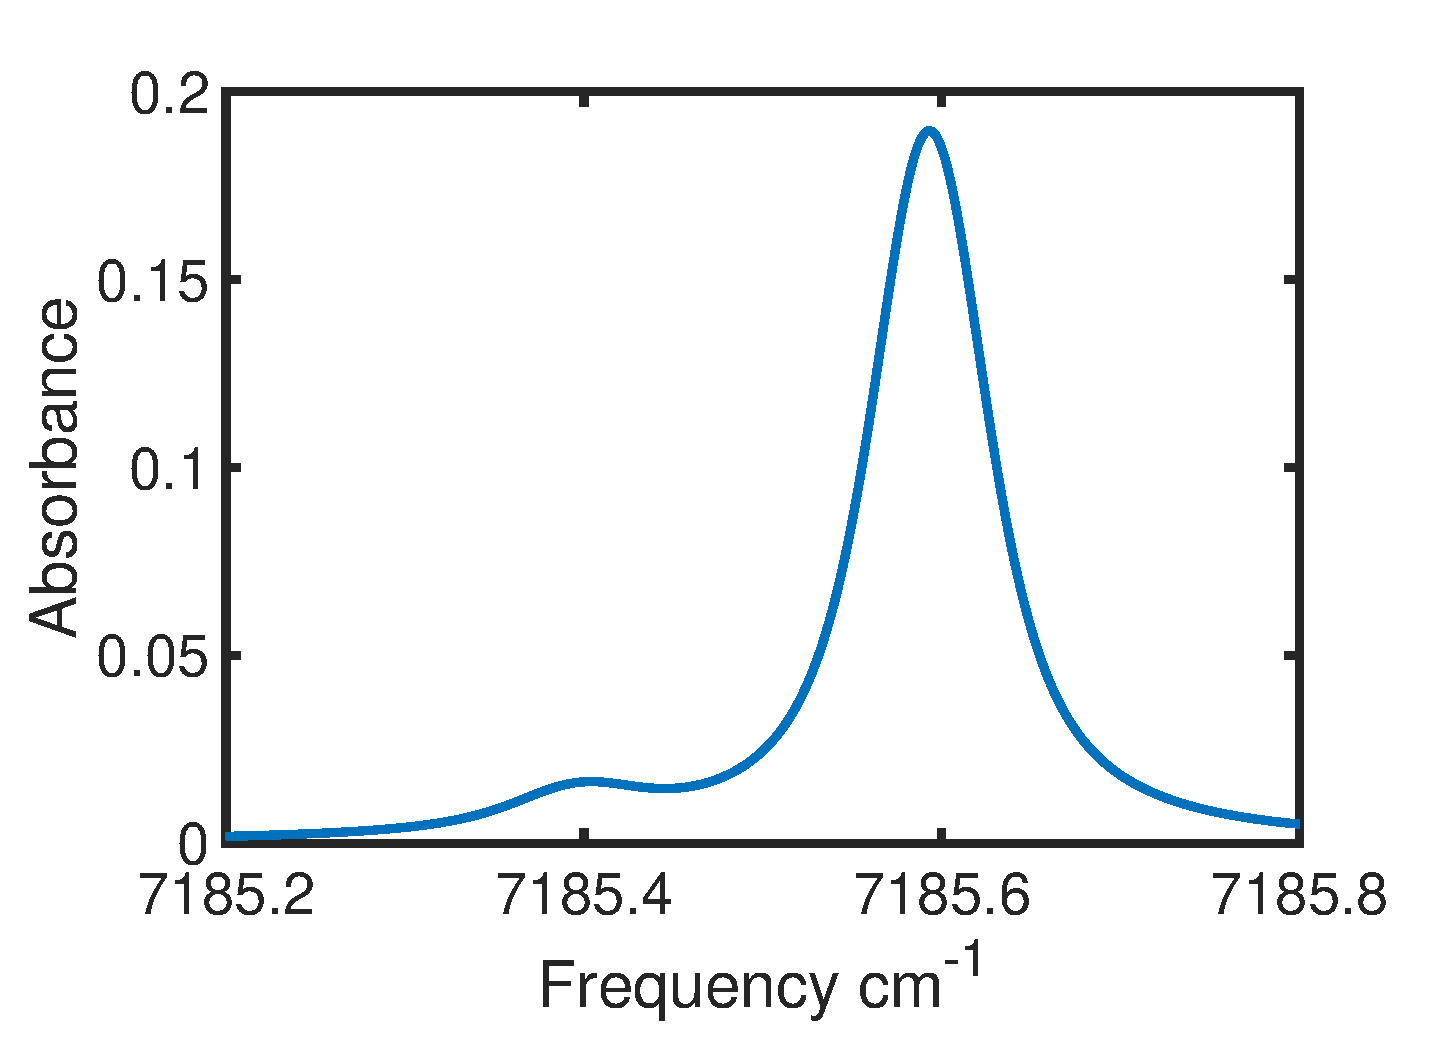
\includegraphics[width=1\textwidth]{fig/ch4_fig3_2.eps}  
\end{minipage} 
\caption{Simulated absorbance spectra of the H2O transitions targeted by the SE-LAS sensor. Simulations performed for a gas at 1000 K and 1 atm with $10\%$ $H_2O$ by mole and a path length of a 7.52 cm.}
    \label{fig:ch4_3}
\end{figure} 


\subsection{Accelerated scanned-WMS-{$2f/1f$} spectral-fitting technique}

To reduce the time required for data processing, a library of scanned-WMS-$2f/1f$ spectra was generated for a given spectroscopic model and set of laser-modulation parameters. It is worth noting that the use of look-up tables to accelerate spectral-fitting routines is a common approach in broadband techniques (e.g., hyperspectral absorption and coherent anti-Stokers Raman scattering), however this has not been used previously in scanned-WMS-$2f/1f$. As a result, the primary value of this work is: 1) describing what level of resolution (within the look-up table) in each spectroscopic parameter is recommended for a given measurement accuracy and 2) quantifying the reduction in computational time associated with this approach. The scanned-WMS-$2f/1f$ simulation technique developed by Goldenstein et al. \cite{Goldenstein2014} was used to simulate scanned-WMS-2f/1f spectra corresponding to each laser and each absorption transition of interest for a fixed Doppler width, $\Delta\nu_D$ (set by the temperature of interest), and numerous values of $A$, $\Delta\nu_C$, and $\nu_0$. Each simulated scanned-WMS-$2f/1f$ spectrum corresponding to a unique combination of $A$, $\Delta\nu_C$, and $\nu_0$ is then stored in a 4-dimensional array, illustrated as a “data block” in Fig. 4.2, with each cell containing a scanned-WMS-$2f/1f$ spectrum spanning a pre-determined frequency/wavelength range (set by the laser scan amplitude, $a_S$). Spectra corresponding to the up-scan and down-scan of the laser’s wavelength are stored separately, since they differ for the same thermodynamic conditions due to the phase shift between the laser’s intensity and wavelength response \cite{Goldenstein2014}.
The resolution of each dimension of the data block (i.e., of each spectroscopic parameter) should be chosen to provide the level of accuracy and precision desired by the user and the size of the library should be large enough to span the range of expected gas conditions. Further, for cases where the Lorentzian-to-Doppler width ratio is near unity, a unique library for every 200 $K$ change in temperature is recommended to account for changes in the Doppler width, although the user should confirm that this provides the desired level of accuracy. For the experiments presented here, the dimensions and resolution of the library were chosen to yield an accuracy of $\approx 1.5\%$. The specific dimensions of each library used here are shown in Table.4.2.

\begin{table}[h]
\begin{center}
\begin{tabular}{ c c c }
\hline
Parameter & Laser: 1392 $nm$  & Laser: 1343 $nm$ \\
 & Min:step:Max & Min:step:Max\\ \hline
$\nu_0$,$cm^{-1}$ & 7185.58:0.001:7185.60 & 7444.34:0.001:7444.36\\ 
$A$,$cm^{-1}$ & 0.022:0.0005:0.035 & 0.015:0.0005:0.0275\\ 
$\Delta\nu_c$,$cm^{-1}\cdot atm^{-1}$ & 0.06:0.00075:0.1 & 0.045:0.00075:0.075\\ \hline
\end{tabular}
\caption{Resolution of spectroscopic parameters used to generate scanned-WMS-$2f/1f$ spectra in the look-up table used by the accelerated scanned-WMS-$2f/1f$ spectral-fitting routine.}
\label{table:ch4_2}
\end{center}
\end{table}

During data processing, a time history of measured scanned-WMS-$2f/1f$ spectra is broken into individual spectra which spans the same frequency/wavelength range as the simulated spectra contained within the scanned-WMS-$2f/1f$ library. The sum-of-squared-error (SSE) between the measured spectrum and all spectra contained in the library is calculated. The spectrum corresponding to the smallest SSE is deemed the best-fit and the coordinates of this spectrum within the library (i.e., data cube) yield the best-fit value of $A$, $\Delta\nu_C$ and $\nu_0$. For the library used here, this operation was completed in ≈0.1 seconds per spectrum using MATLAB R2014b on a MacBook Pro with a 2.3 $GHz$ Intel Core $i$5 processor. 

\noindent This method is 100$x$ faster than the WMS-$2f/1f$ spectral-fitting routines developed previously \cite{Goldenstein2014}. For large datasets, the approach described here is critical to performing data processing on a personal computer. For example, in the experiments conducted here, approximately 240,000 scanned-WMS-$2f/1f$ spectra were processed to characterize the burner operation over a 30-minute period. Using conventional fitting methods this would have required nearly 28 days of computational time. In comparison, using the scanned-WMS-2f/1f library the dataset was processed in 6.6 hours of computational time.

 \begin{figure}[h]
    \centering       
    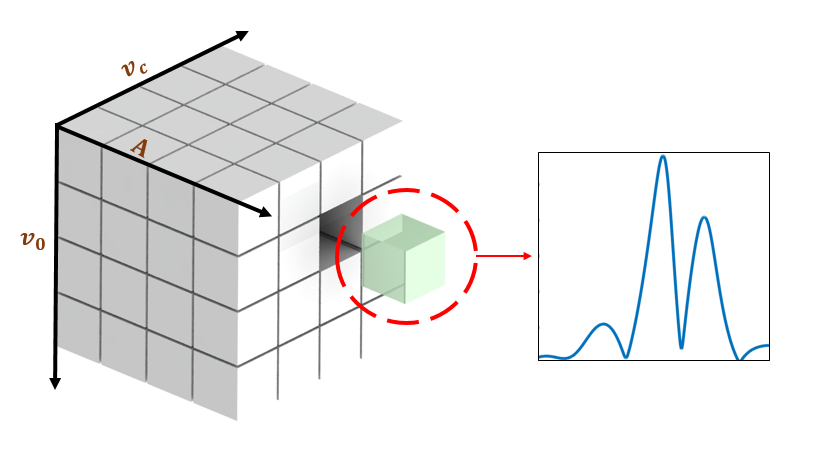
\includegraphics[width=0.7\textwidth]{fig/ch4_fig4.png}
        \caption{Concept schematic of look-up table used by accelerated scanned-WMS-$2f/1f$ spectral-fitting routine.}
    \label{fig:ch4_2}
\end{figure}


\section{Sensor Architecture}
\subsection{Experimental setup}

Fig. 4.3 illustrates a schematic of the experimental setup used to provide measurements of temperature and $H_2O$ concentration in a propane-air burner using the SE-LAS sensor. Two distributed-feedback (DFB) tunable diode lasers in a fiber pigtail configuration were multiplexed using a 2-by-2 fiber multiplexer. One arm of the fiber multiplexer was used to direct laser light to a conventional line-of-sight sensor (not shown here, see Fig. 4.7) and the other arm was connected to the fiber bundle utilized by the SE-LAS sensor. The fiber bundle was connected to the SE-LAS sensor housing (details provided in the following subsection) which was threaded directly into the wall of a stainless-steel propane-air burner. The burner has a 3" inner diameter and the inner surface of the burner has a matte finished (i.e., it is not polished). For the line-of-sight sensor, two NPT pipe plugs containing 0.5" diameter, sapphire windows were threaded into the burner wall. A type-$K$ thermocouple was used to monitor the burner’s exterior wall temperature adjacent to the SE-LAS sensor. The fiber bundle (Neptec OS) contains a single SMF-28 fiber (for transmitting laser light) which is surrounded by 6 multimode fibers (105 $\mu m$ core diameter, $NA=0.22$) for collecting the backscattered laser light and directing it to a photodetector. A lens doublet containing two aspheric lenses (Thorlabs C330TMD-C, $f=3.10 \,mm$, $d=6.33 \,mm$, $NA=0.68$) mounted in a cage system was used to collimate the light exiting the fiber bundle and focus it onto the detector (Thorlabs PDA10CS). The detector was operated with a gain of 30 $dB$, yielding a bandwidth of 775 $kHz$. The detector signal was recorded at 10 $MS/s$ on a 12 bit data acquisition card (GaGe CSE123G2).

 \begin{figure}[ht]
    \centering
        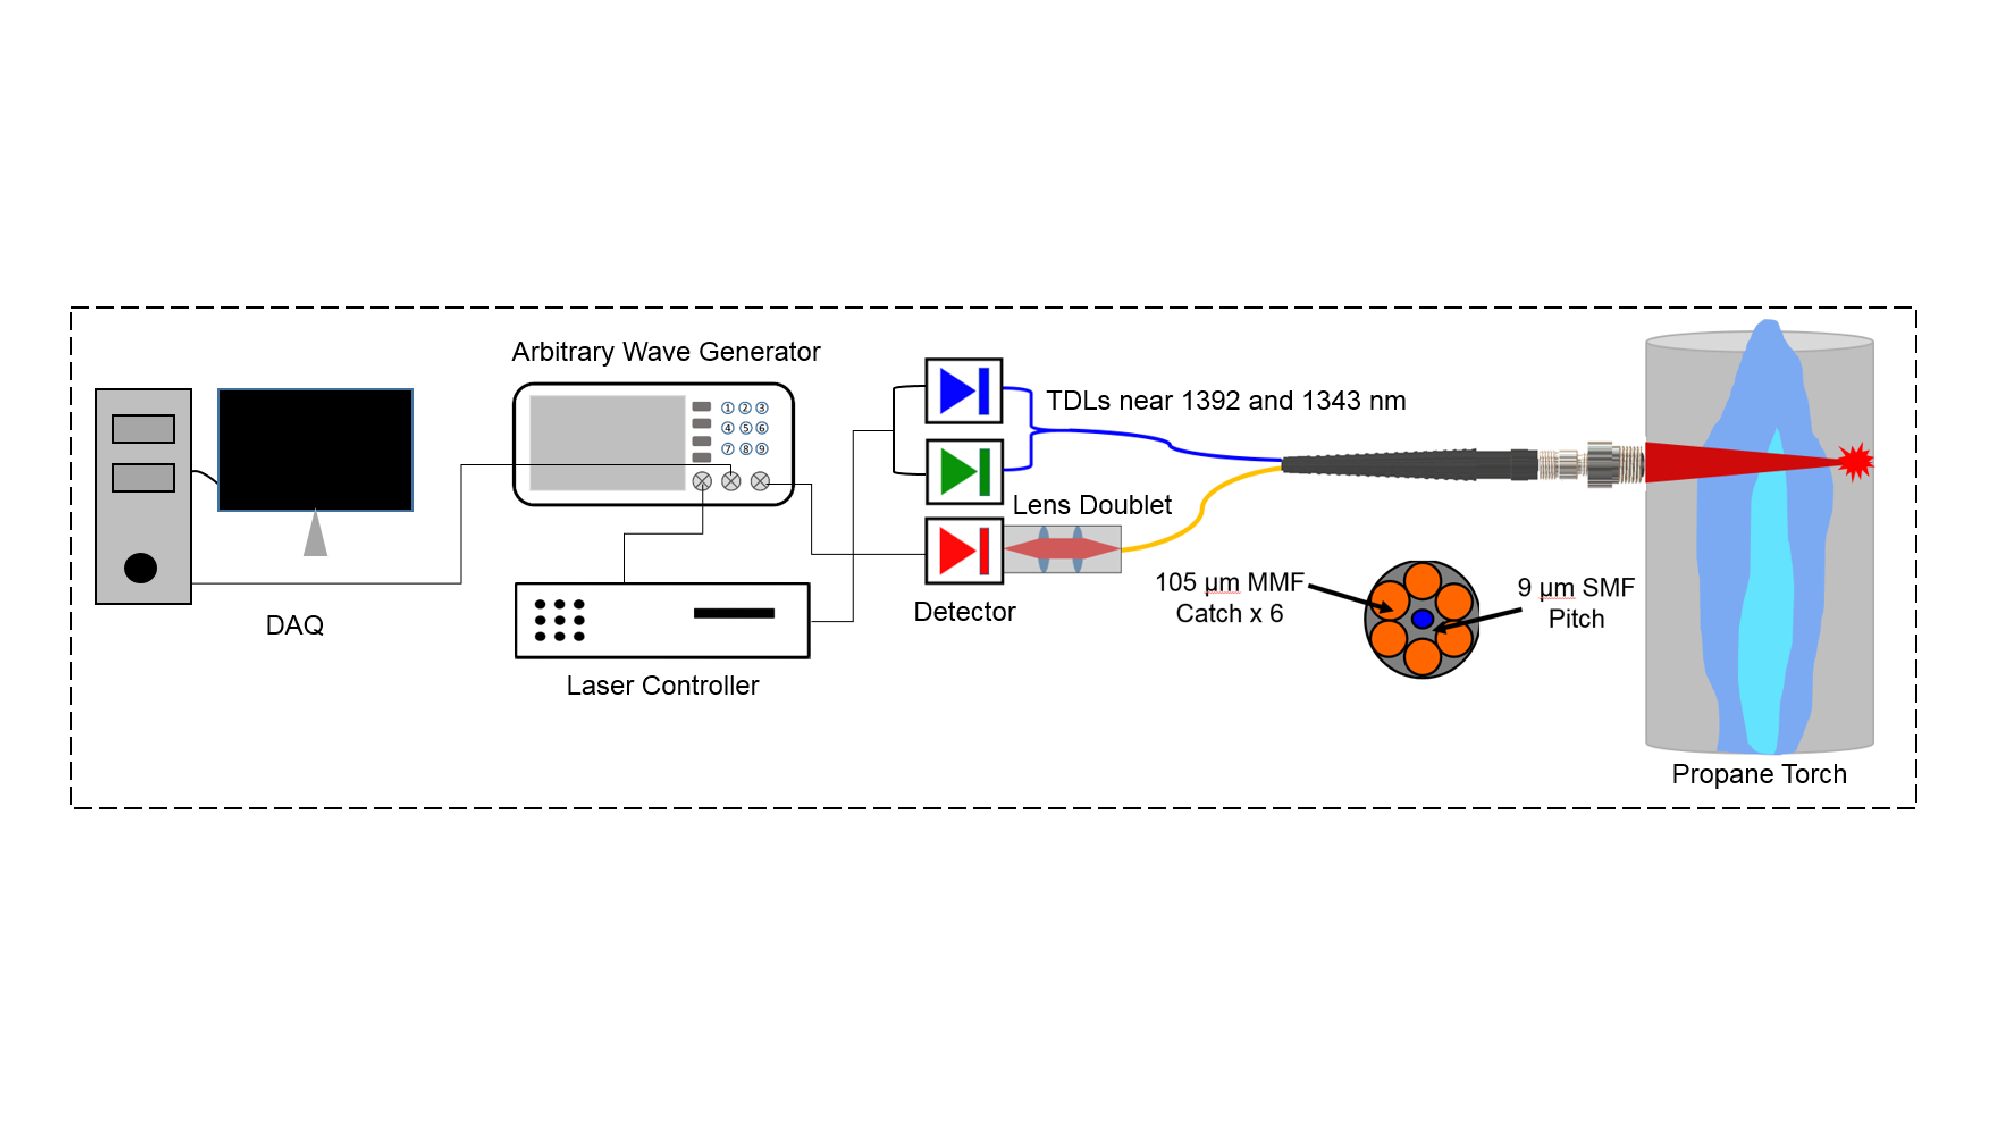
\includegraphics[trim = 0mm 52mm 0mm 20mm, clip=true, width=1\textwidth]{fig/ch4_fig1.pdf}
        \caption{Schematic of experimental setup used to measure temperature and $H_2O$ with the single-ended laser-absorption sensor.}
    \label{fig:ch4_3}
\end{figure}

The nominal temperature and current of the lasers were controlled by a commercially available laser controller (ILX Lightwave LDC3916372) and current modulation was achieved by applying a voltage modulation (generated by a 14-bit arbitrary waveform generator, Tektronix AFG 3252) to the modulation port on each laser’s controller card. During scanned-WMS experiments, the current of both lasers was scanned using a 1 $kHz$ sinewave while the laser near 1392 nm was modulated at 160 $kHz$ and the laser near 1343 nm was modulated at 200 $kHz$. The scan amplitude ($\sim 0.2 cm^{-1}$) was chosen to enable each laser to be scanned across their respective absorption transitions, and the modulation amplitudes (0.09 $cm^{-1}$ for 1392 $nm$ laser and 0.08 $cm^{-1}$ for 1343 $nm$ laser) were chosen to maximize the WMS-$2f$ signal of each laser at the nominal test conditions. The same modulation parameters were used in fixed-WMS experiments.


\subsection{Design of SE-LAS sensor housing}

 \begin{figure}[h]
    \centering
        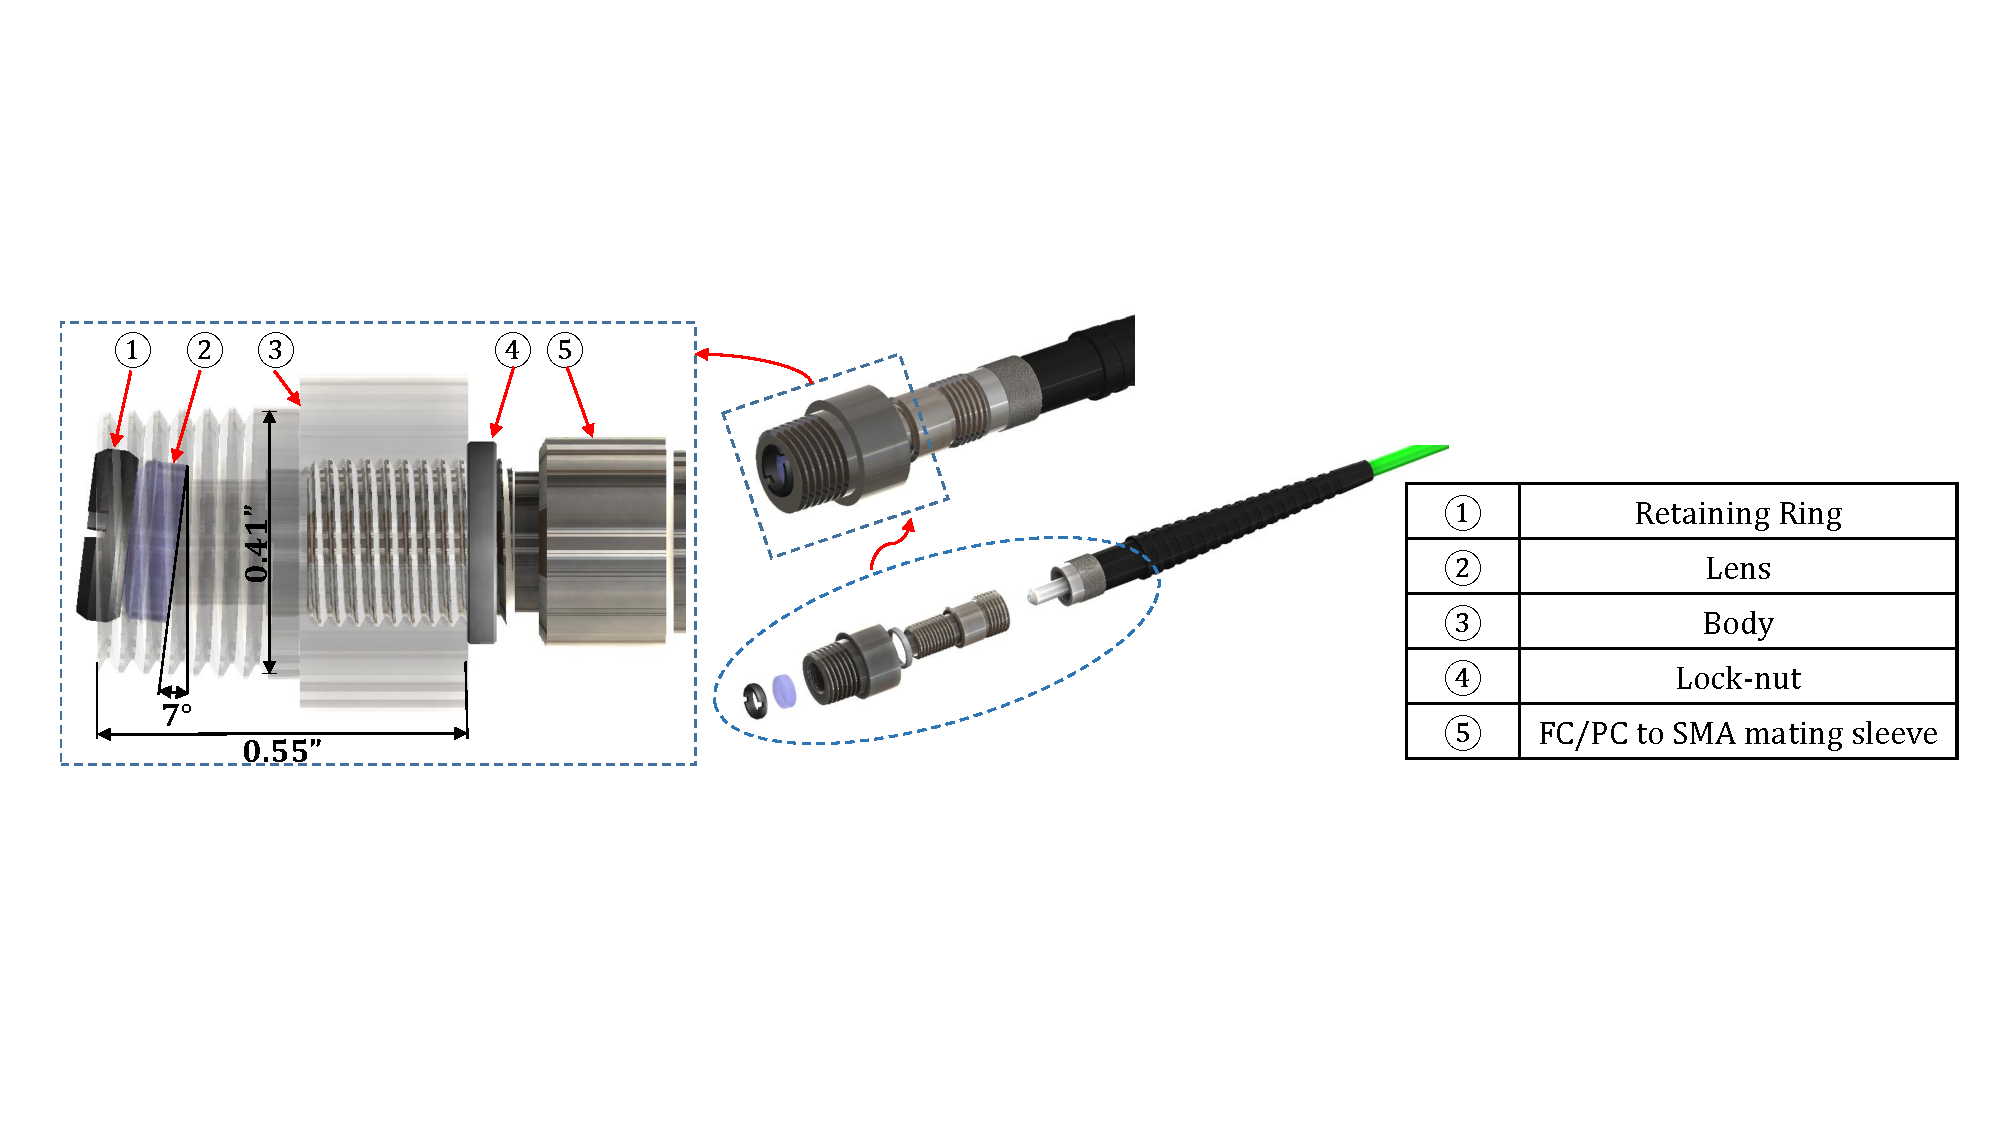
\includegraphics[trim = 0mm 52mm 0mm 20mm, clip=true, width=1\textwidth]{fig/ch4_fig2.pdf}
        \caption{CAD rendering of SE-LAS sensor housing and exploded view illustrating key components.}
    \label{fig:ch4_4}
\end{figure}


A CAD rendering illustrating the SE-LAS sensor housing is shown in Fig. 4.4. The sensor housing consists of: 1) a retaining ring with $M6.5\times 0.5$ threads (Thorlabs SM6RR), 2) an anti-reflection (AR) coated, BK7, plano-convex lens with a diameter of 6 mm and focal length of 15 $mm$ (Thorlabs: LA1222-C), 3) a custom stainless-steel body, 4) a lock-nut, and 5) a standard FC/PC to SMA mating sleeve (Thorlabs ADAFCSMA1). All parts, excluding the sensor body, are commercially available. The sensor body was custom made from a 316 stainless-steel rod and is 0.55" long with an outer diameter of 0.45". This sensor housing provides a 9$x$ smaller sensor footprint compared to that used in \cite{Goldenstein:16}. The sensor body has $1/8$" NPT external threads to enable convenient and sealed installation into the burner. The retaining ring ($M6.5 \times 0.5$ threads) was used to secure the lens to a shoulder tilted at $7^{\circ}$ relative to the optical axis in order to prevent collection of light reflected off the lens surface. The position of the fiber tip was adjusted to focus the laser light onto the target (i.e., the burner wall) which leads to maximum light collection efficiency \cite{Goldenstein:16}. Once the optimum location of the fiber tip was determined, the fiber position was locked in place using the lock-nut fastened to the FC/PC to SMA mating sleeve. Once locked in place, the SE-LAS sensor housing could be repeatedly removed and installed in the burner without compromising the light collection efficiency.


\subsection{SE-LAS Sensor design challenges}
Several design challenges were overcome to achieve a compact SE-LAS sensor that is suitable for direct exposure to high-temperature gases.

1. Miniaturize sensor housing: Reducing the size of the SE-LAS sensor housing introduced several design challenges which were addressed by careful selection of the lens parameters and housing dimensions. First, the distance between the fiber tip and lens was chosen such that the beam exiting the fiber does not diverge beyond the clear aperture of the system. This is required to ensure maximum optical throughput and prevent reflections within the sensor housing which could be collected by the fiber bundle and lead to unwanted background signals. This matter is further complicated by the fact that the distance between the lens and fiber tip must be chosen such that the lens focuses the transmitted light onto the scattering target to ensure maximum collection efficiency. As such, the focal length, clear aperture, and distance between fiber and lens must all be chosen together.
Second, miniaturizing the sensor housing corresponds to reducing the distance between the fiber tip and lens. This increases the amount of reflected light (off the lens surface) that is collected by the fiber bundle leading to unwanted background signals. This challenge was avoided here by mounting the lens on a shoulder that is tilted at $7^{\circ}$ relative to the optical axis, thereby directing the reflected beam outside the fiber bundle’s collection angle. It should be noted that this design element is necessary despite using an AR-coated lens with $\approx 0.3\%$ reflectance at the laser operating wavelengths. Using this arrangement, the amount of light that was reflected off the lens and collected by the fiber bundle was less than $0.5\%$ of that which was backscattered off the burner surface and collected.
Last, miniaturizing the sensor housing requires using a smaller lens which could reduce the amount of backscattered light that is collected by fiber bundle. However, despite using an 18$x$ smaller lens, our design provided a collection efficiency equal to 0.5 times that reported in \cite{Goldenstein:16} for a 15 $cm$ standoff distance. Given the similar optical design between these two SE-LAS sensors, this small difference in collection efficiency can be explained by recognizing that the fiber bundle accepts only a relatively small “cone” of backscattered light. As a result, using a larger lens does not provide much added benefit at the standoff distances studied here.

2. Extend sensor housing to high-temperature combustion environments: Several factors were considered to ensure that the SE-LAS could withstand direct exposure to high-temperature combustion gases for long durations. First, the lens must be able to withstand its peak operating temperature without melting or eroding in the presence of hot water vapor. This prohibits use of $CaF_2$ and other fluoride crystals which are hygroscopic and, thus, cannot withstand exposure to high-temperature water vapor as encountered here. Here, AR-coated BK7 was used due to its low cost ($\approx \$$30 USD), sufficiently high melting temperature ($\approx 830 \,K$), and ability to withstand exposure to hot water vapor. For higher-temperature and -pressure environments and/or mid-infrared applications, AR-coated sapphire lenses offer a better alternative due to its extremely high melting temperature ($\approx 2300\, K$), larger strength, resistance to thermal shock, and ability to tolerate hot combustion gases. However AR-coated sapphire lenses suitable for this SE-LAS sensor are not commercially available. Last, the body of the sensor housing should be constructed from a machinable material that has a relatively low thermal conductivity. This is required to insulate the fiber bundle from high temperatures since it is constructed using epoxy and plastics which cannot withstand temperatures greater than 150 C. Here, 316 stainless steel was used for the sensor body instead of aluminum due to its $\approx 15x$ smaller thermal conductivity. This was sufficient to prevent the FC/PC to SMA mating sleeve (i.e., the fiber bundle’s mating surface) from exceeding a temperature of 80 C. For higher-temperature environments, machinable ceramics may be a more suitable material.

3. Mitigate Cavity Noise: The SE-LAS sensor generates optical cavity noise since the incident and backscattered laser light overlap on each other and the optical coherence is sufficiently preserved after the reflection. As a result, during scanned-wavelength experiments, interference fringes can appear in the collected laser light as shown in \cite{Goldenstein:16}. To mitigate this noise source, WMS-$2f/1f$ is performed using modulation frequencies above 100 $kHz$ as recommended in \cite{Goldenstein:16}. Despite this added noise source and $100x$ lower optical throughput, the use of WMS-$2f/1f$ enables the SE-LAS sensor to provide measurements of temperature and $H_2O$ concentration with a comparable or better precision compared to a traditional line-of-sight-based LAS sensor (see Section 4.4.2).



\section{Experimental Results}
\subsection{Collection efficiency}
The collection efficiency of the SE-LAS sensor was measured as a function of standoff distance (i.e., working distance) for different reflectors/scattering targets to evaluate its optical design and operating limits. The distance between the SE-LAS sensor and aluminum (unpolished/mill finish with and without soot) and paper targets was varied by placing the SE-LAS sensor housing on a translation stage. A fiber-coupled power meter was used to measure both the optical power exiting the fiber bundle and the amount of backscattered optical power that was collected by the 6 MMF within the fiber bundle. Fig. 4.5 shows the fraction of light collected as a function of standoff distance. For the experiment and modulation setpoints used here, the quality of WMS-$2f/1f$ spectra degraded significantly when the fraction of light collected fell below $10^{-3}$. This coupled with the results shown in Fig. 4.5 indicates that the SE-LAS sensor (as presented here) should be capable of successful operation at standoff distances up to 100 $cm$. The fraction of light collected follows a power law decay (exponent near -1.7) with increasing standoff distance. The addition of soot (deposited using a rich propane flame) to the aluminum target (Fig. 4.6) reduced the fraction collected by only a factor of 5. This indicates that the SE-LAS sensor presented here should be robust against some degree of soot decomposition on combustor walls. Interestingly, for the clean aluminum target, teh SE-LAS sensor presented here yields a collection that is 50$\%$ (at $L=15$ $cm$) and 30$\%$ (at $L=100$ $cm$) of that shown in \cite{Goldenstein:16} where a 18$x$ larger lens (1" diameter) was used. However, for the paper target, the larger lens used in \cite{Goldenstein:16} yields a collection efficiency that is typically 10 times larger than that presented here. These results suggest that using a larger lens becomes increasingly more important as the standoff distance is increased or for backscattering targets that yield more diffuse reflections.

\vspace{3mm}

 \begin{figure}[h]
    \centering
        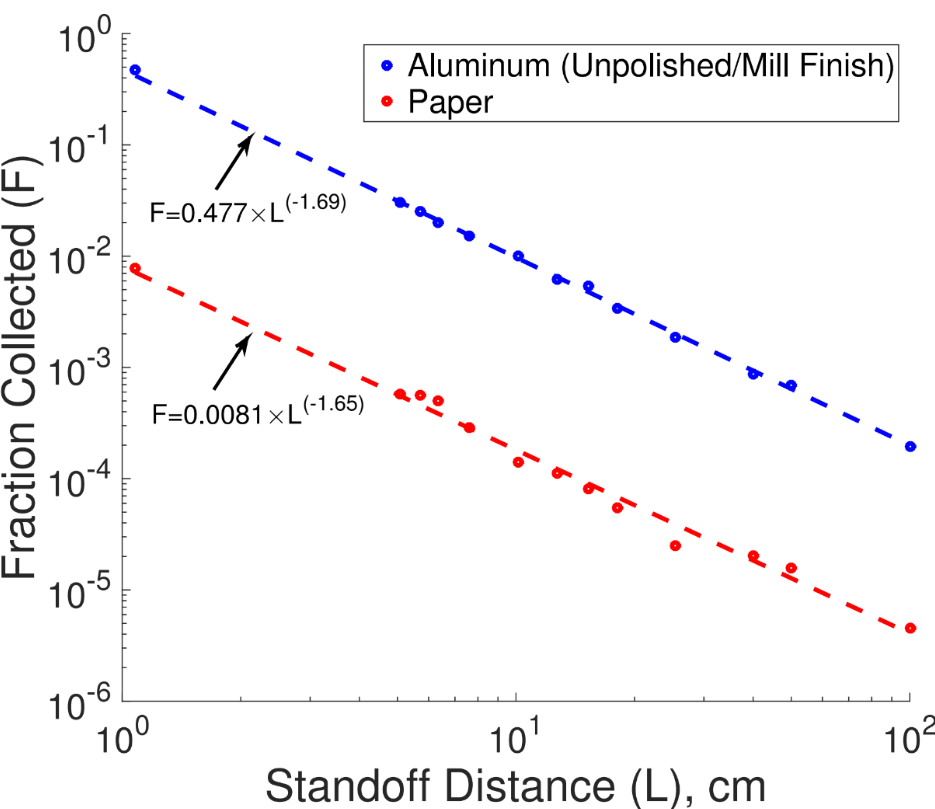
\includegraphics[width=0.5\textwidth]{fig/ch4_fig11_v2.png}
        \caption{Fraction of light collected by SE-LAS sensor as a function of standoff distance for aluminum and paper backscattering targets.}
    \label{fig:ch4_5}
\end{figure}

 \begin{figure}[h]
    \centering
        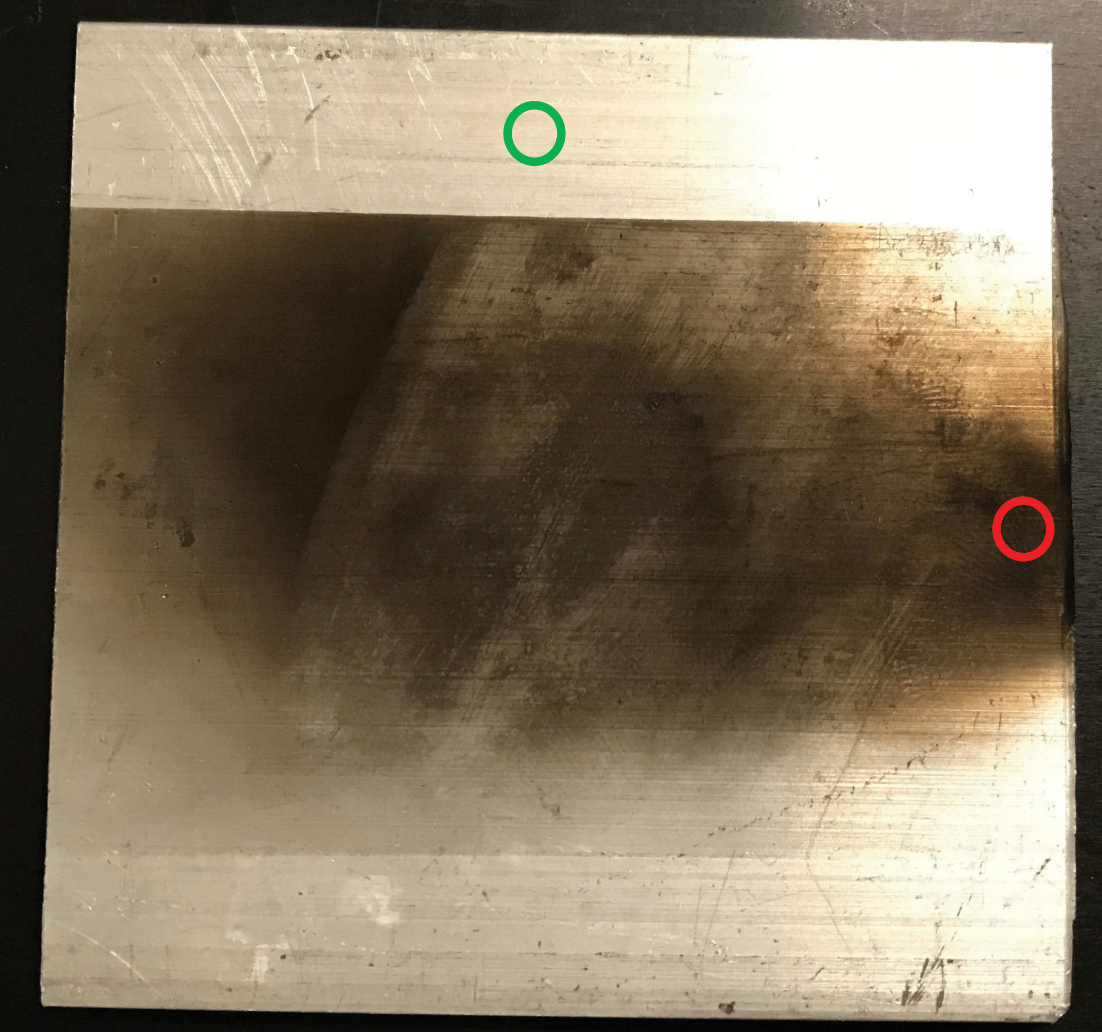
\includegraphics[width=0.4\textwidth]{fig/ch4_fig12.png}
        \caption{Photo of aluminum backscattering target. Green and red rings illustrate the laser beam location for comparing the fraction of light collected from backscattering off clean and soot-coated aluminum, respectively.}
    \label{fig:ch4_6}
\end{figure}


\subsection{Combustion experiments}
Experiments were conducted with the burner and LAS sensors operating in two modes: 1) Fixed-WMS experiments were conducted to resolve a transient ignition blast and 2) scanned-WMS experiments were conducted over a period of 30 minutes to monitor the quasi-steady behavior of the burner and proof-test the SE-LAS sensor in a high-temperature environment for a long duration. Fig. 4.7 illustrates the burner operating with both the line-of-sight LAS sensor and the single-ended LAS sensor installed on the burner body. Fig. 4.7(a) and Fig. 4.7(c) illustrate the burner during an ignition blast and the quasi-steady operation that follows, respectively.

 \begin{figure}[b]
    \centering
        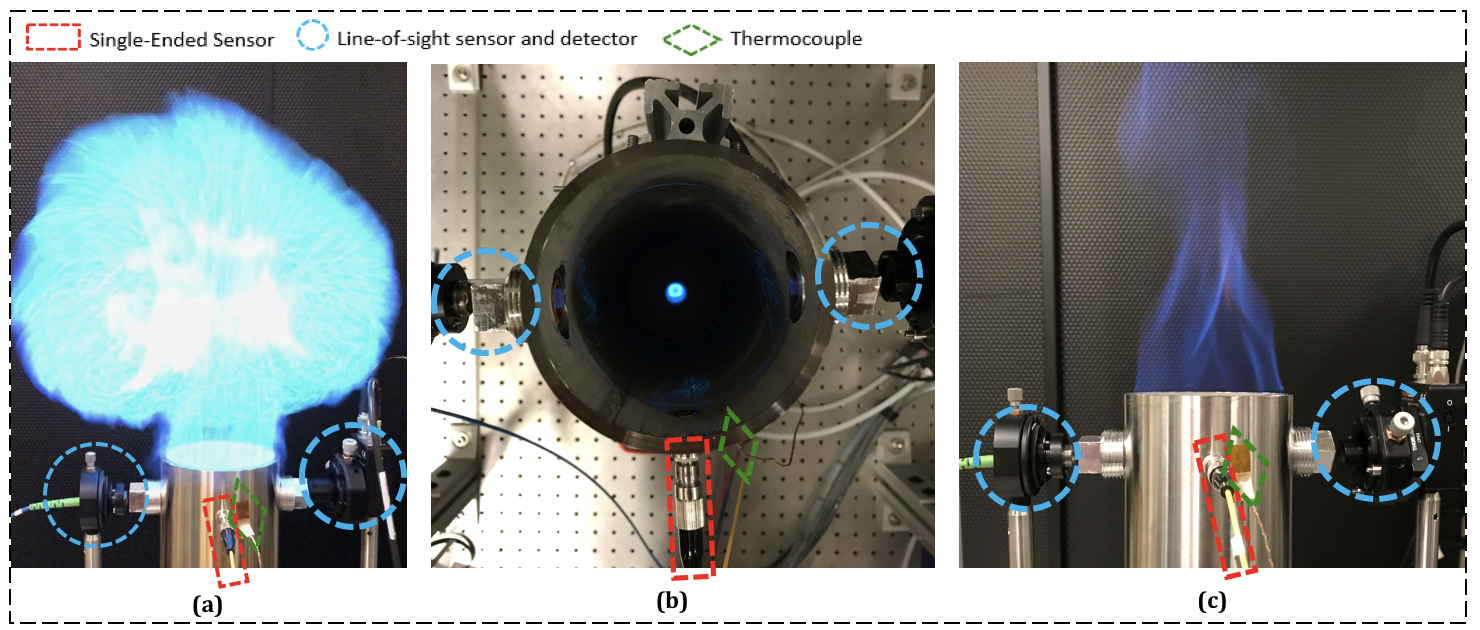
\includegraphics[width=1\textwidth]{fig/ch4_fig6_v3.png}
        \caption{Photos of propane-air burner during operation with LAS sensors and thermocouple installed. The photos illustrate the burner during an ignition blast (a), with a small throttled flame (b), and during quasi-steady state at full throttle (c).}
    \label{fig:ch4_7}
\end{figure}

Fig. 4.8 illustrates measured temperature time histories for both sensors during an ignition blast. The measurements were acquired using fixed-WMS-$2f/1f$ with 25 $kHz$ lock-in filters (applied during post-processing) to provide a measurement bandwidth of 25 $kHz$ (analogous to a 50 $kHz$ measurement rate). The results indicate excellent agreement between both sensors and suggest that the temperature field is axisymmetric during the test. The measured temperature time histories agree within 10 $K$ of each other and exhibit a $1\sigma$ precision of 22 $K$ (line-of-sight sensor) and 26 $K$ (single-ended sensor). These results suggest that our single-ended sensor offers comparable accuracy and precision to conventional line-of-sight sensors despite 100$x$ lower optical throughput (i.e., collection efficiency).

\begin{figure}[b]
    \centering
        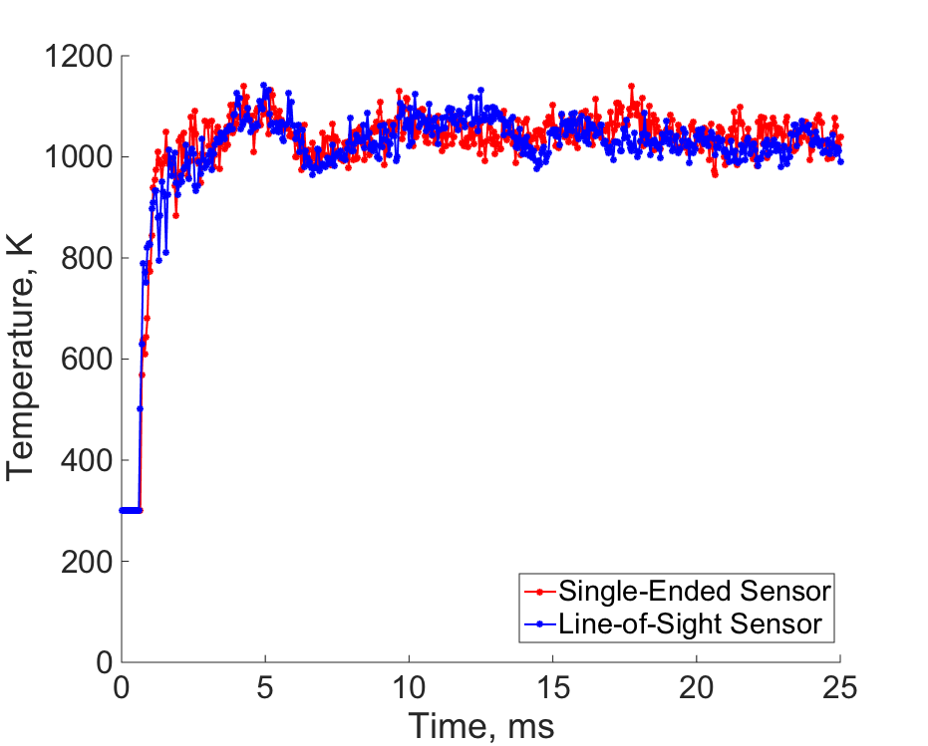
\includegraphics[width=0.6\textwidth]{fig/ch4_fig7.png}
        \caption{Temperature time histories measured during a burner ignition event using single-ended and line-of-sight LAS sensors and fixed-WMS-$2f/1f$ with a measurement bandwidth of 25 $kHz$.}
    \label{fig:ch4_8}
\end{figure}

\begin{figure} \centering 

\begin{subfigure}[b]{0.475\linewidth}  
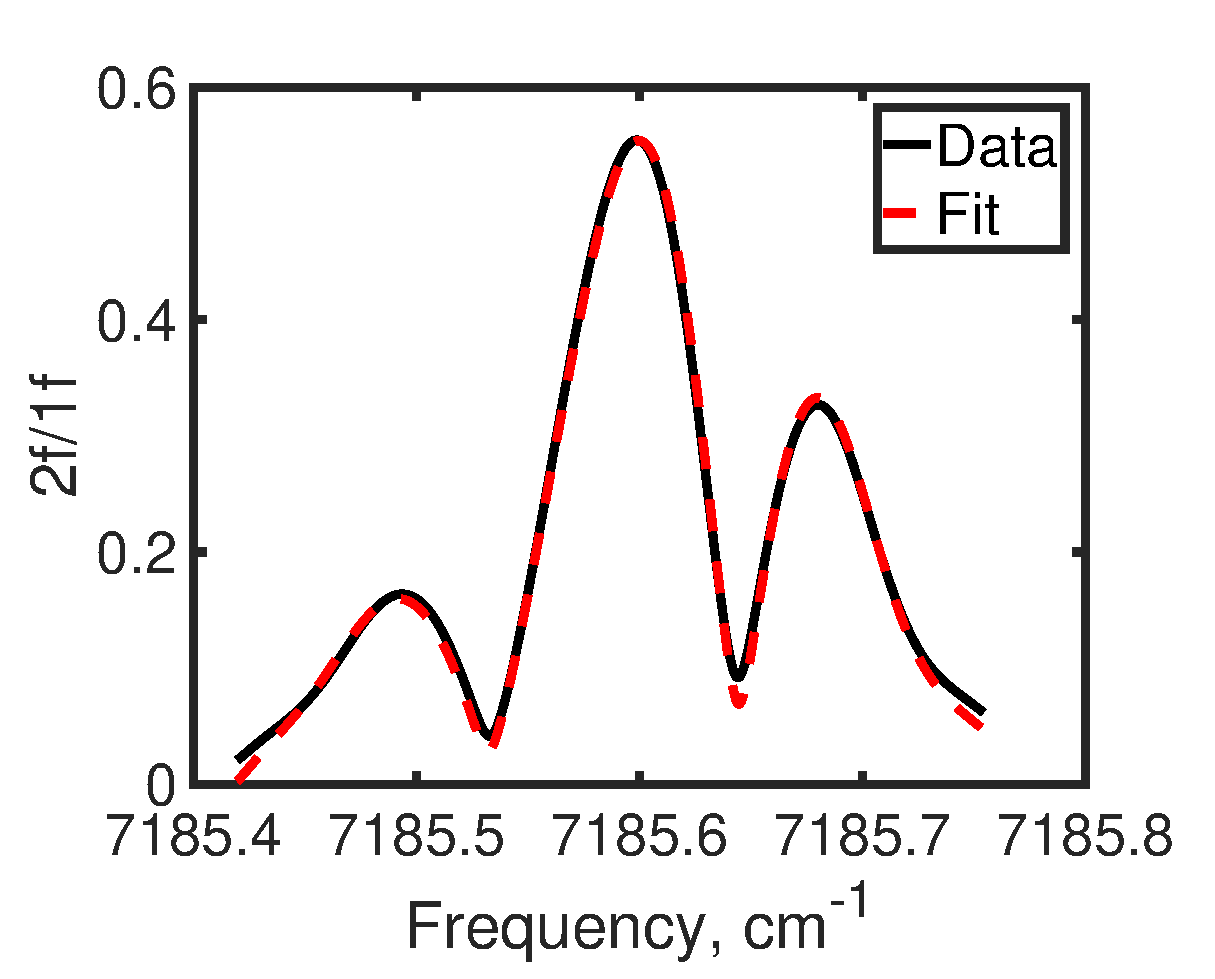
\includegraphics[width=\textwidth]{fig/LOS_1392_fit.eps}  
\end{subfigure}%  
\hfill
\begin{subfigure}[b]{0.475\linewidth}  
\centering  
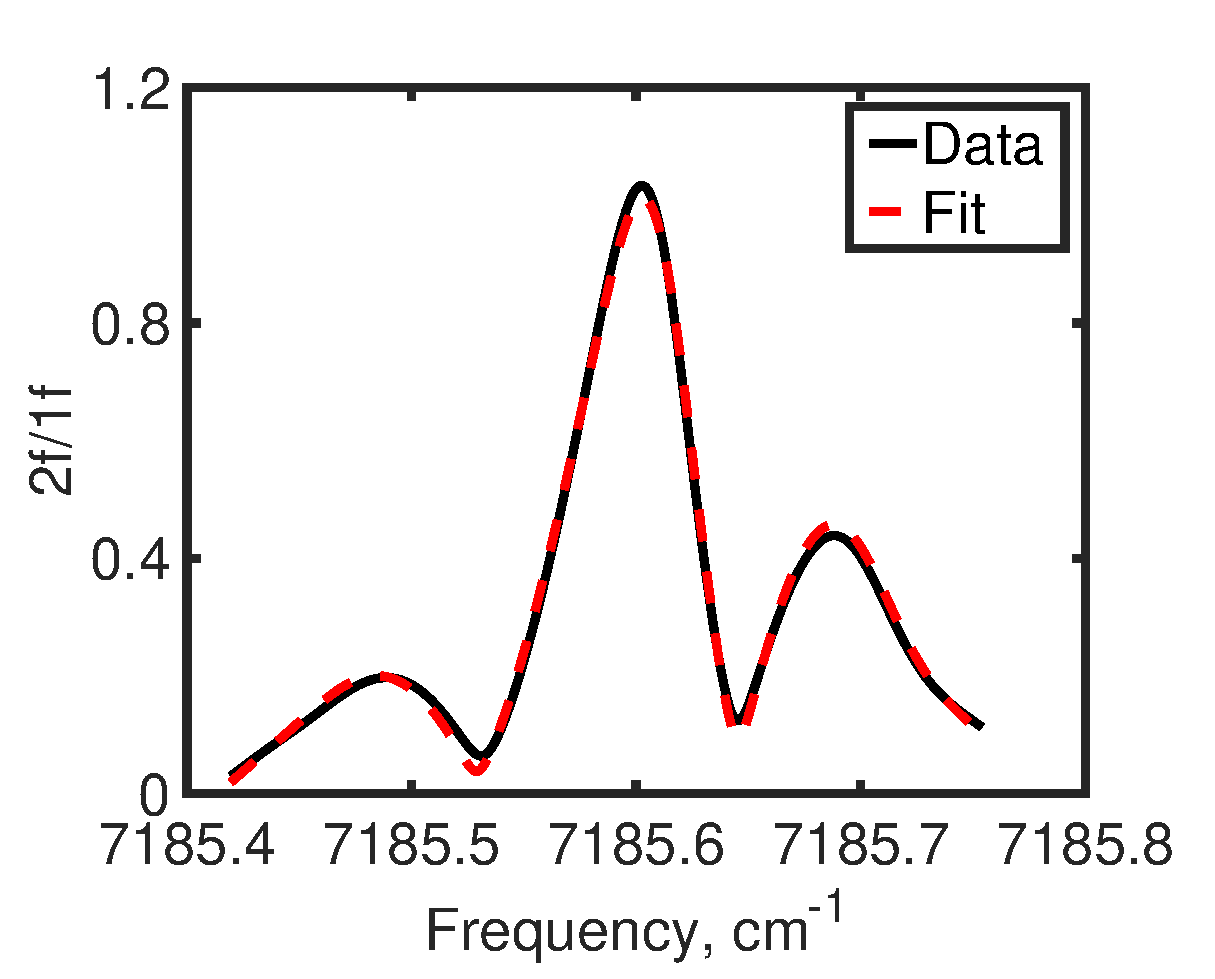
\includegraphics[width=\textwidth]{fig/SE_1392_fit.eps}  
\end{subfigure} 

\vskip\baselineskip
\begin{subfigure}[b]{0.475\linewidth}  
\centering  
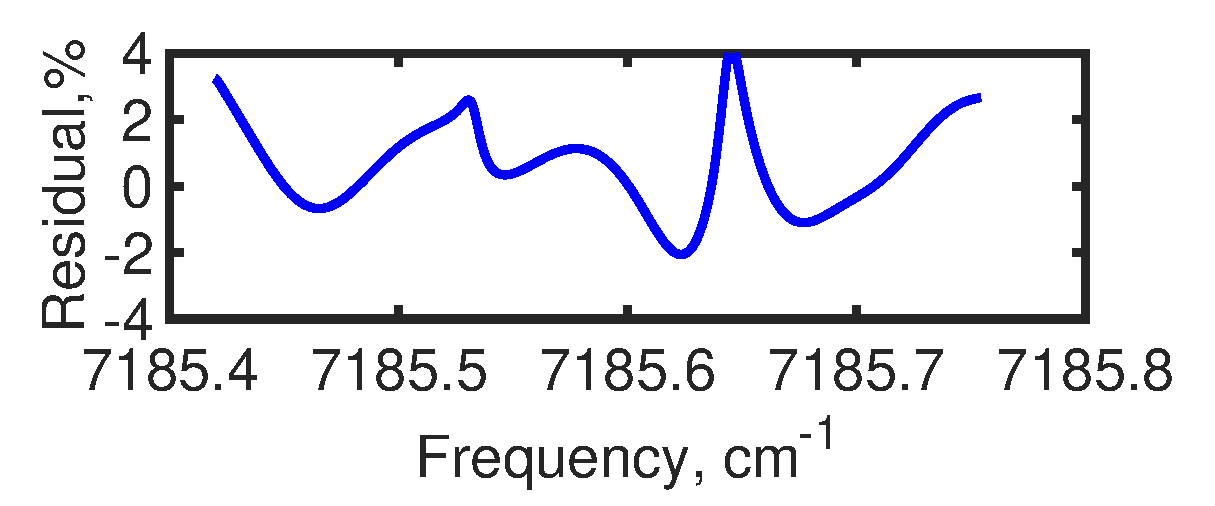
\includegraphics[width=\textwidth]{fig/LOS_1392_residual.eps}  
\caption{\underline{1392 nm: LOS}}
\end{subfigure} 
\quad
\begin{subfigure}[b]{0.475\linewidth}  
\centering  
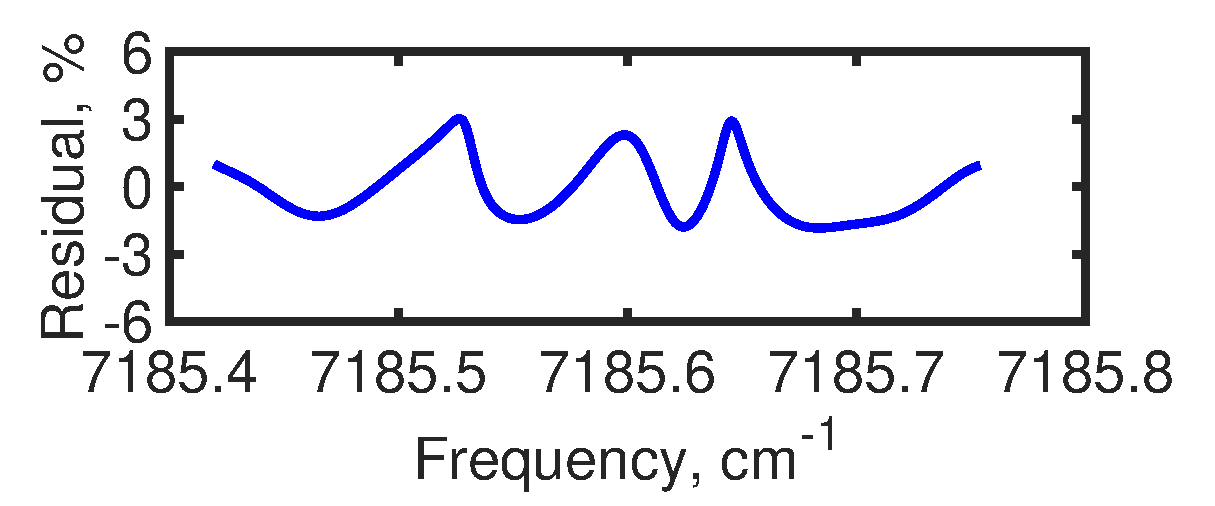
\includegraphics[width=\textwidth]{fig/SE_1392_residual.eps}  
\caption{\underline{1392 nm: SE}}
\end{subfigure} 

\begin{subfigure}[b]{0.475\linewidth}  
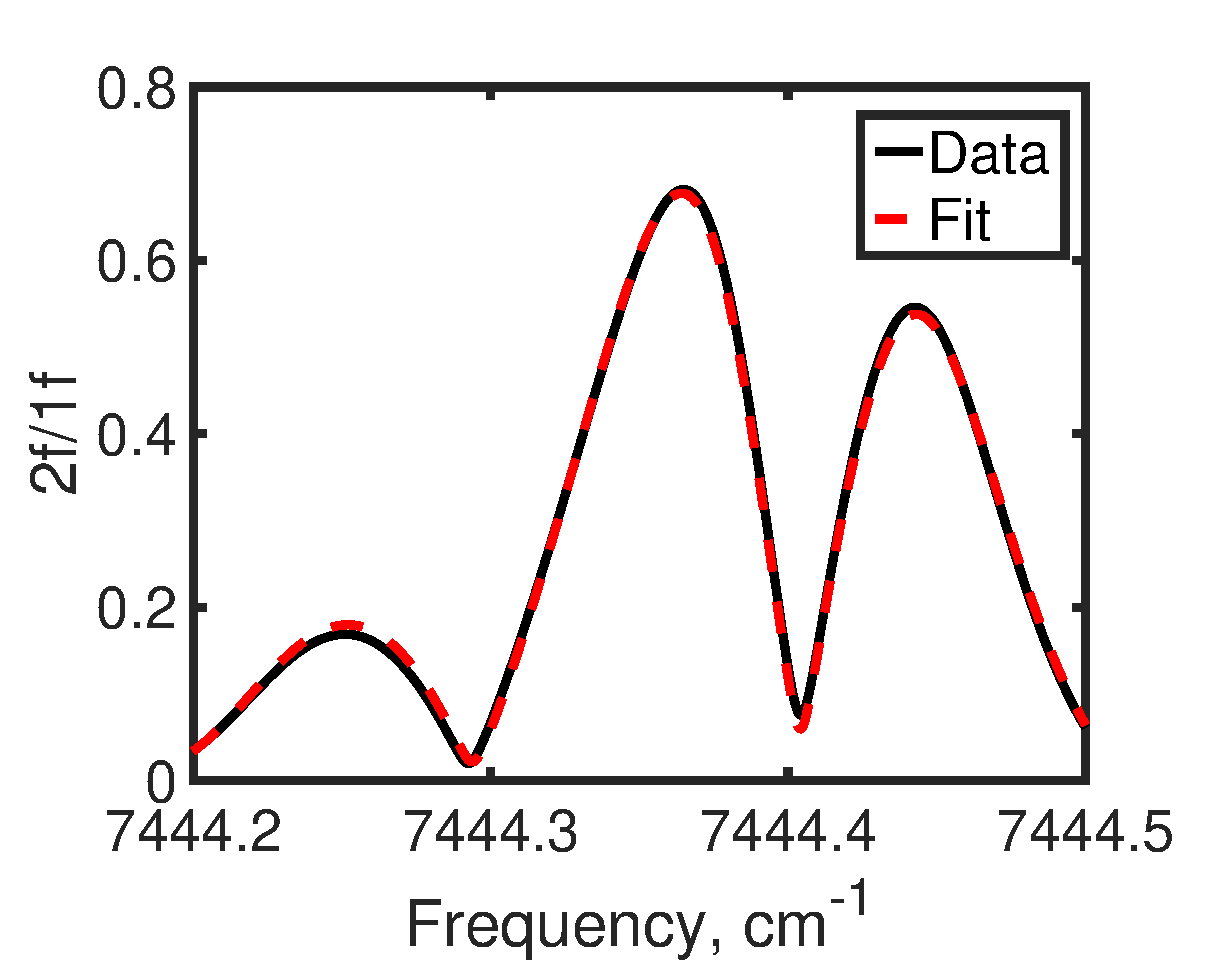
\includegraphics[width=\textwidth]{fig/LOS_1343_fit.eps}  
\end{subfigure}%  
\hfill
\begin{subfigure}[b]{0.475\linewidth}  
\centering  
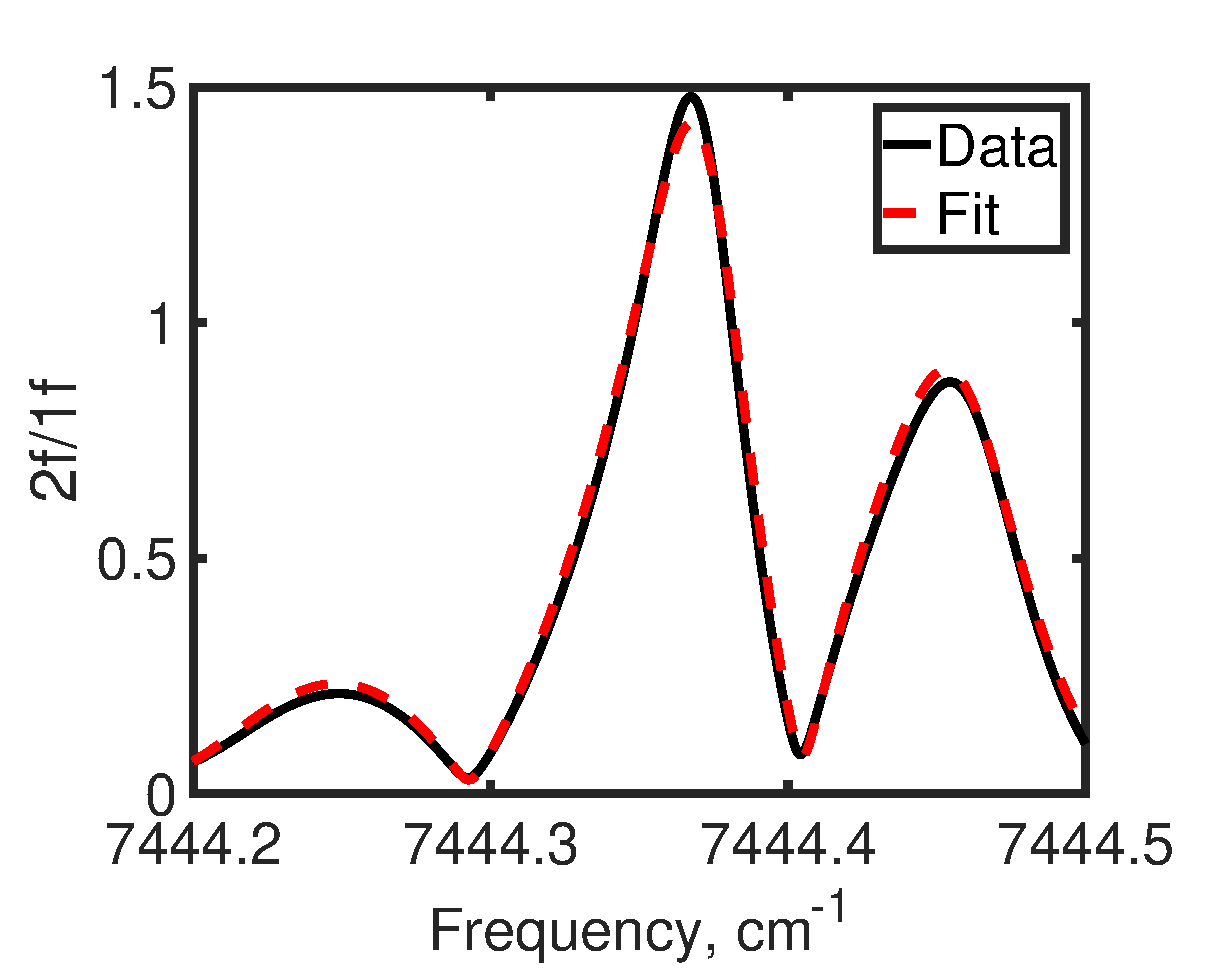
\includegraphics[width=\textwidth]{fig/SE_1343_fit.eps}  
\end{subfigure} 

\vskip\baselineskip
\begin{subfigure}[b]{0.475\linewidth}  
\centering  
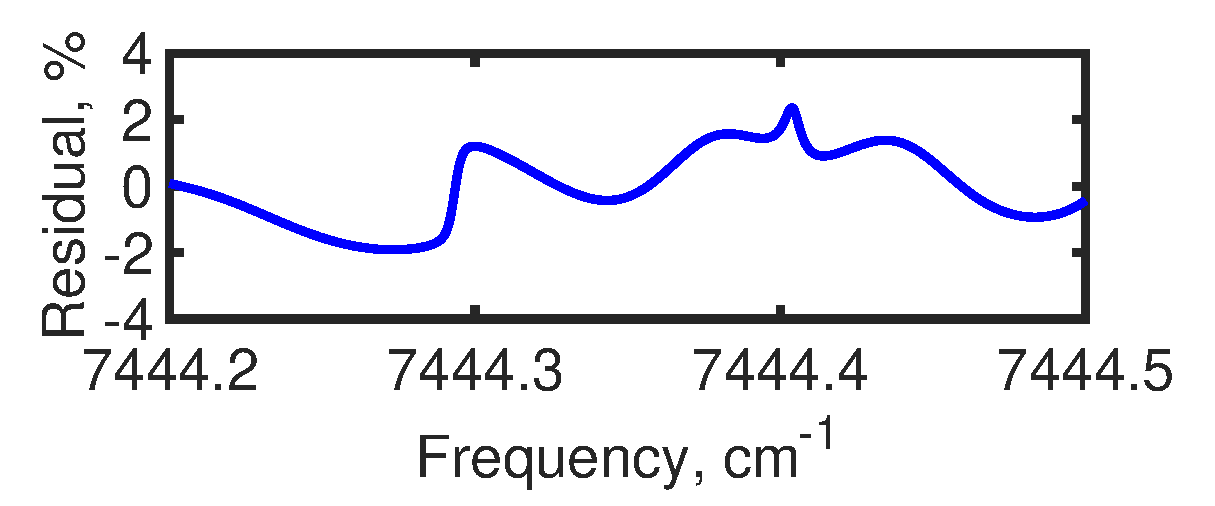
\includegraphics[width=\textwidth]{fig/LOS_1343_residual.eps}  
\caption{\underline{1343 nm: LOS}}
\end{subfigure} 
\quad
\begin{subfigure}[b]{0.475\linewidth}  
\centering  
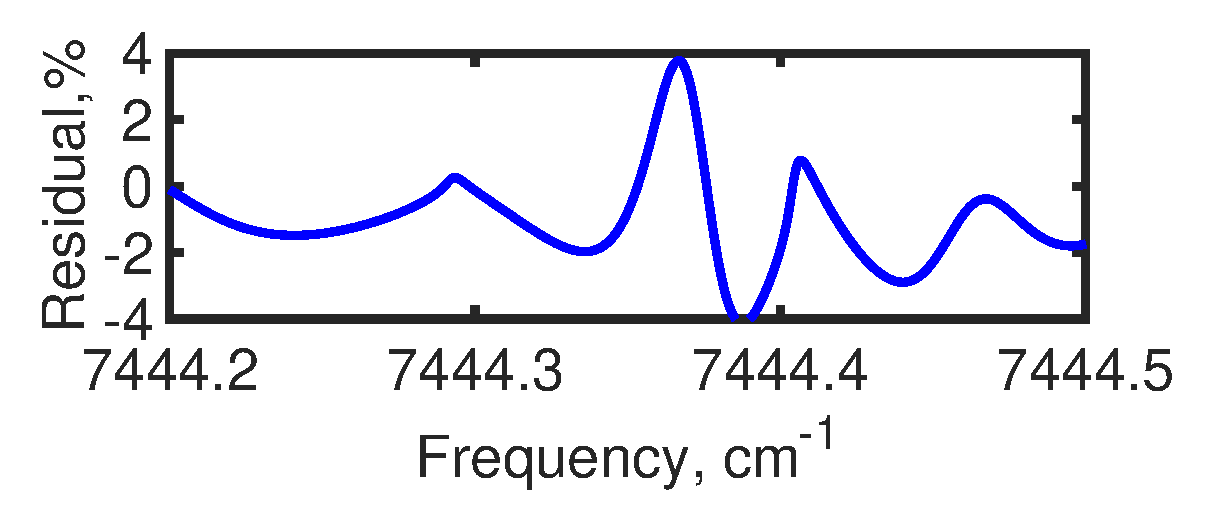
\includegraphics[width=\textwidth]{fig/SE_1343_residual.eps}  
\caption{\underline{1343 nm: SE}}
\end{subfigure} 

\caption{Example of measured and best-fit scanned-WMS-$2f/1f$ spectra for each laser and both LAS sensors (line-of-sight (LOS) and single-ended (SE)) with the burner operating at quasi-steady state.}
    \label{fig:ch4_8}
\end{figure}

Scanned-WMS-$2f/1f$ measurements of gas temperature and $H_2O$ mole fraction were acquired using the LOS- and SE-LAS sensors over a 30 minute period with the burner operating at quasi-steady state. This experiment was conducted to: 1) evaluate the performance of the SE-LAS sensor over an extended period of time in a high-temperature environment and 2) evaluate the accuracy and precision of the SE-LAS sensor while utilizing scanned-WMS-$2f/1f$ spectral fitting. To prevent excessive data collection, approximately 1 second of data was recorded once per minute for 30 minutes for each LAS sensor. The burner wall temperature was also recorded each minute to provide a conservative estimate for the temperature of the SE-LAS sensor’s lens and to establish when the burner walls reached a steady-state temperature. 

Fig. 4.9 illustrates a single scanned-WMS-$2f/1f$ spectrum and its best fit for each laser acquired using both the SE-LAS and LOS-LAS sensor with the burner operating at quasi-steady state (nominal gas conditions of approximately 1000 $K$ and 13$\%$ $H_2O$ by mole). The best-fit scanned-WMS-$2f/1f$ spectra were determined using the accelerated fitting routine described in Section 4.2.3. 


For both LAS sensors, the best-fit spectra provide peak-normalized residuals typically within $2\%$, although residuals as large as $4\%$ occur at isolated frequencies for the SE-LAS sensor. The performance of both sensors is consistent with that provided by previously developed line-of-sight-based sensors using scanned-WMS-2f/1f spectral fitting techniques \cite{Makowiecki2017,Goldenstein2014,goldenstein2014scanned,spearrin2014simultaneous}. These results indicate that our SE-LAS and accelerated scanned-WMS-$2f/1f$ spectral-fitting routine provide scanned-WMS-$2f/1f$ measurements of gas temperature and $H_2O$ mole fraction with an accuracy that is comparable to that of previously developed LAS sensors requiring optical access with an unobstructed line-of-sight.

For each one-second experiment, the accelerated scanned-WMS spectral-fitting routine was individually applied to all 2000 scanned-WMS-$2f/1f$ spectra (for each laser). The integrated absorbance corresponding to each best-fit spectrum was used to determine the gas temperature and $H_2O$ mole fraction at each moment in time as described in \cite{Goldenstein2014}. Fig. 4.10 shows a portion of a temperature and $H_2O$ mole fraction time history for both sensors.

\begin{figure} \centering 
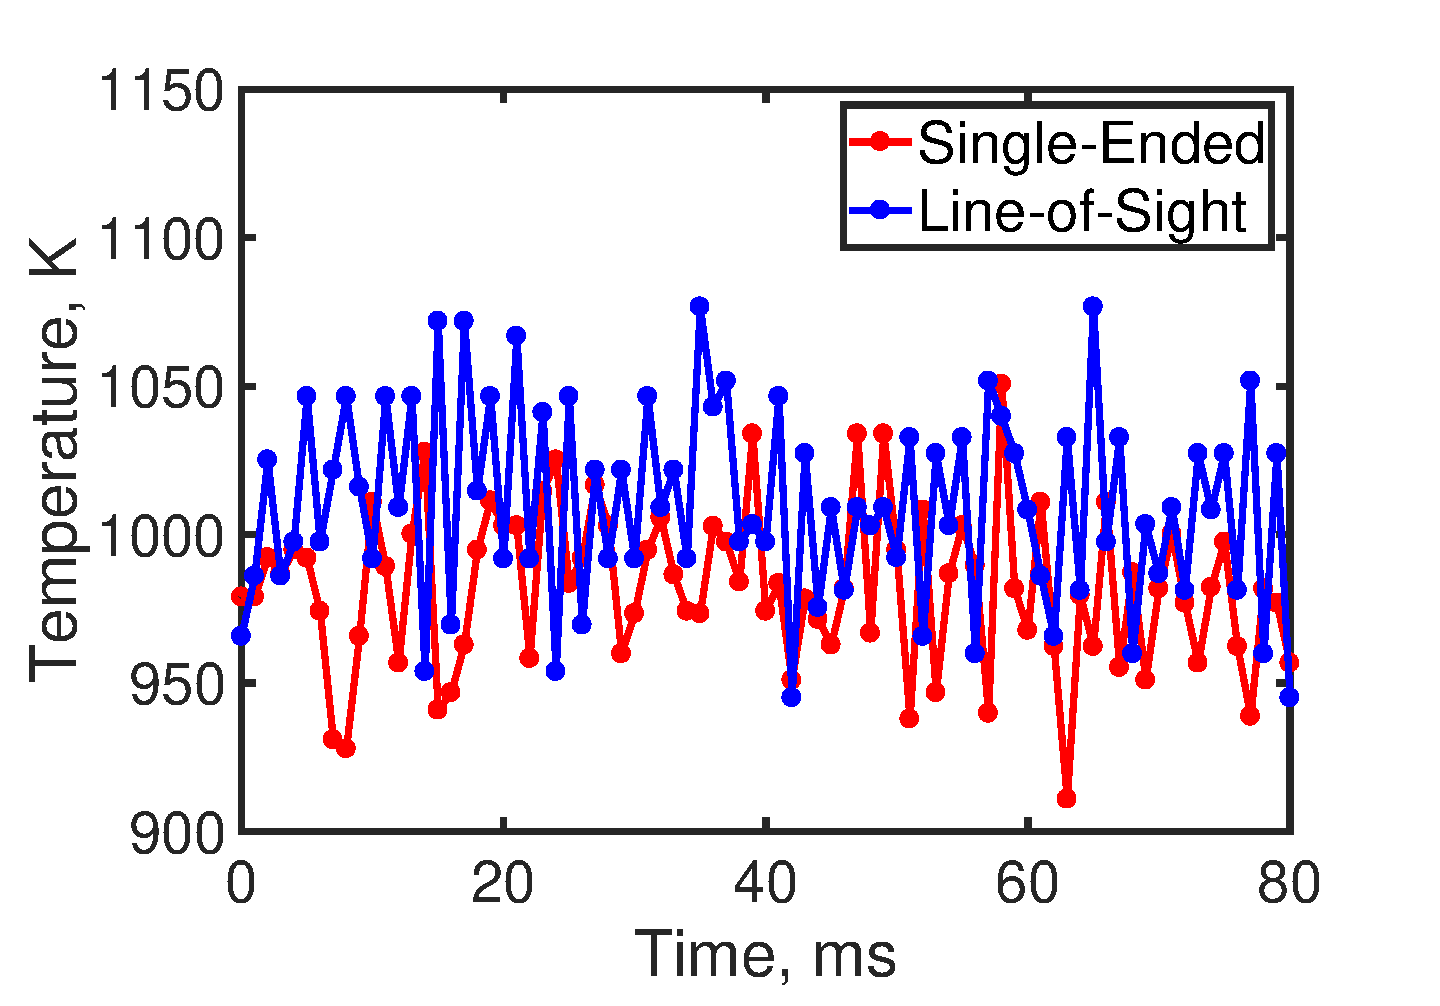
\includegraphics[width=0.7\textwidth]{fig/ch4_fig9_2.eps}  
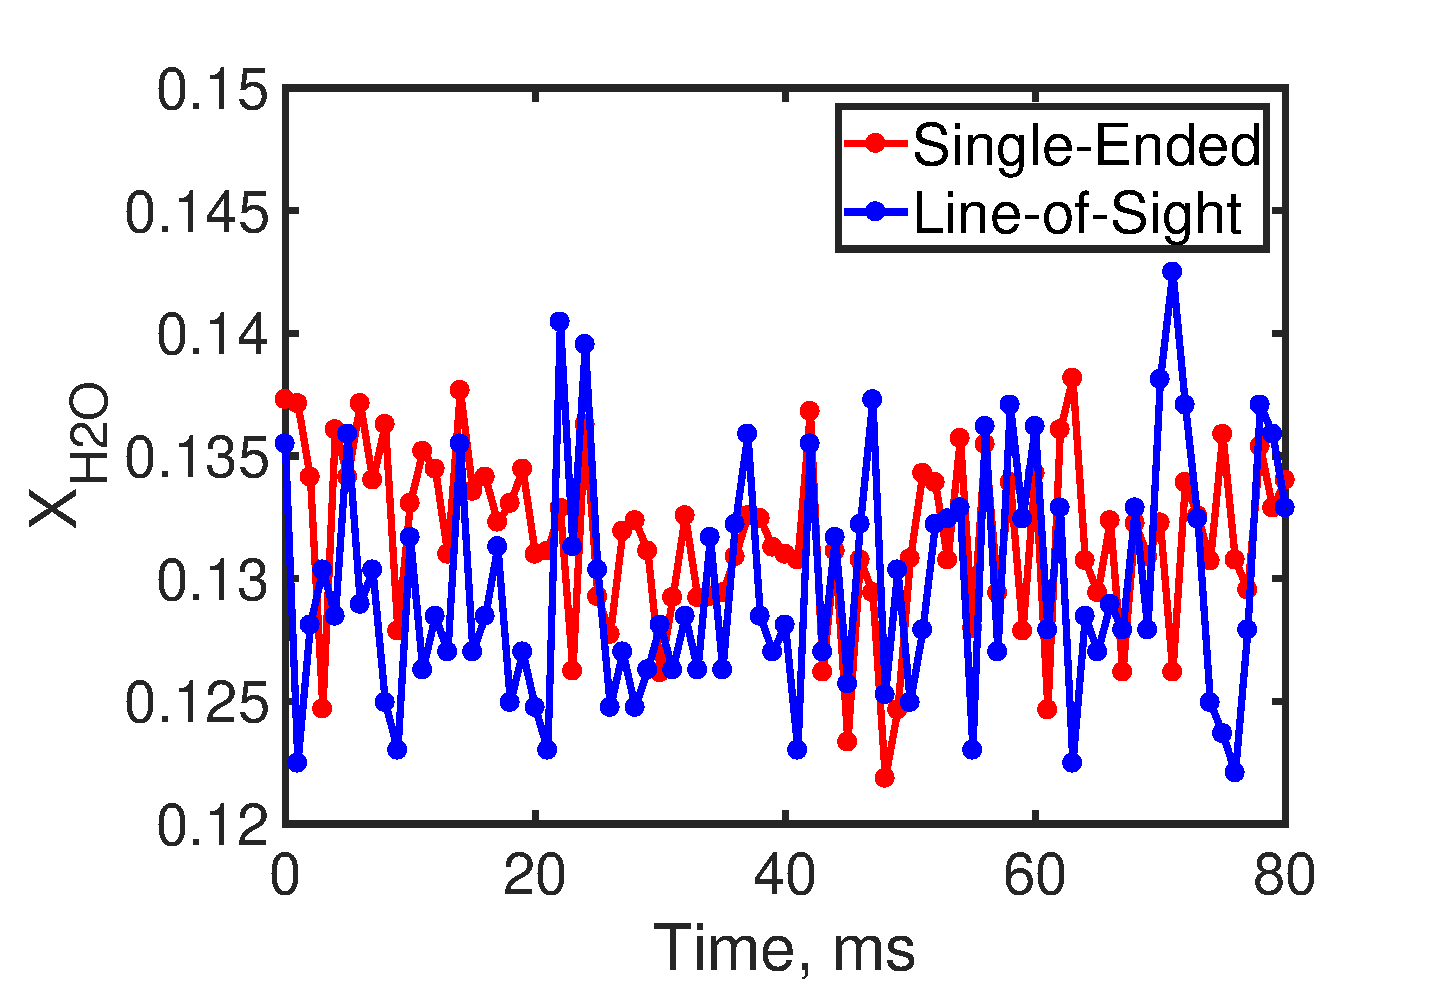
\includegraphics[width=0.7\textwidth]{fig/ch4_fig9_1.eps}  
\caption{Measurements of temperature and $H_2O$ mole fraction acquired at 2 kHz using both LAS sensors and the scanned-WMS-$2f/1f$ spectral fitting with the burner operating at quasi-steady state. Both sensors agree well and the SE-LAS sensor exhibits superior precision.}
    \label{fig:ch4_10}
\end{figure}



The temperature and $H_2O$ mole fraction time histories agree well between both sensors with a mean difference of 28.3 $K$ and 0.0005, respectively. Further, the SE-LAS sensor exhibited a superior $1\sigma$ measurement precision for temperature (26 $K$ compared to 32 $K$ for the LOS-LAS sensor) and $H_2O$ mole fraction (0.0037 compared to 0.0046 for LOS-LAS sensor). The improved precision of the SE-LAS sensor may result from its 2$x$ larger path length which leads to WMS-$2f/1f$ signals that are 2$x$ larger than those of the LOS-LAS sensor (see Fig. 4.9). 

\vspace{15mm}

\noindent The measured time histories illustrate that the gas temperature and $H_2O$ mole fraction are quasi-steady, however moderate fluctuations (compared to the precision observed during the ignition blast) between individual measurements exist. This likely results from swirl- and turbulence-induced fluctuations in combustion progress and heat transfer losses that have taken place leading up to the measurement plane. Visible imaging of the burner interior revealed pronounced swirling structures within the combustor which can also be observed by monitoring the flame at the burner exit plane (see Fig. 4.7(c)).

\begin{figure} \centering 
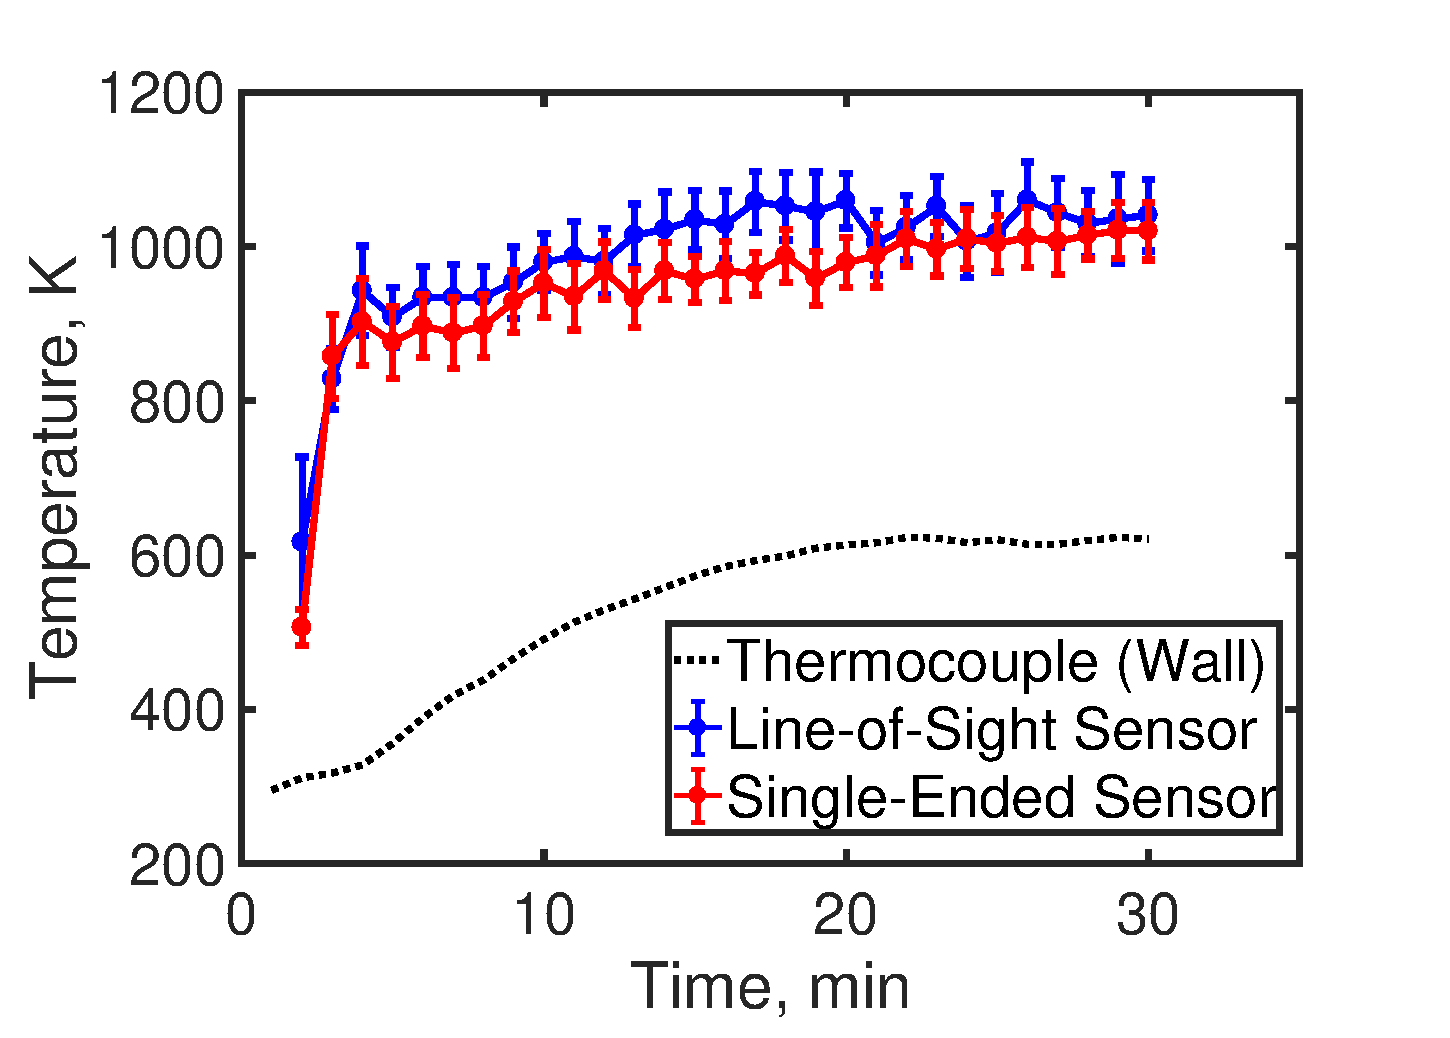
\includegraphics[width=0.7\textwidth]{fig/ch4_fig10_2.eps}  
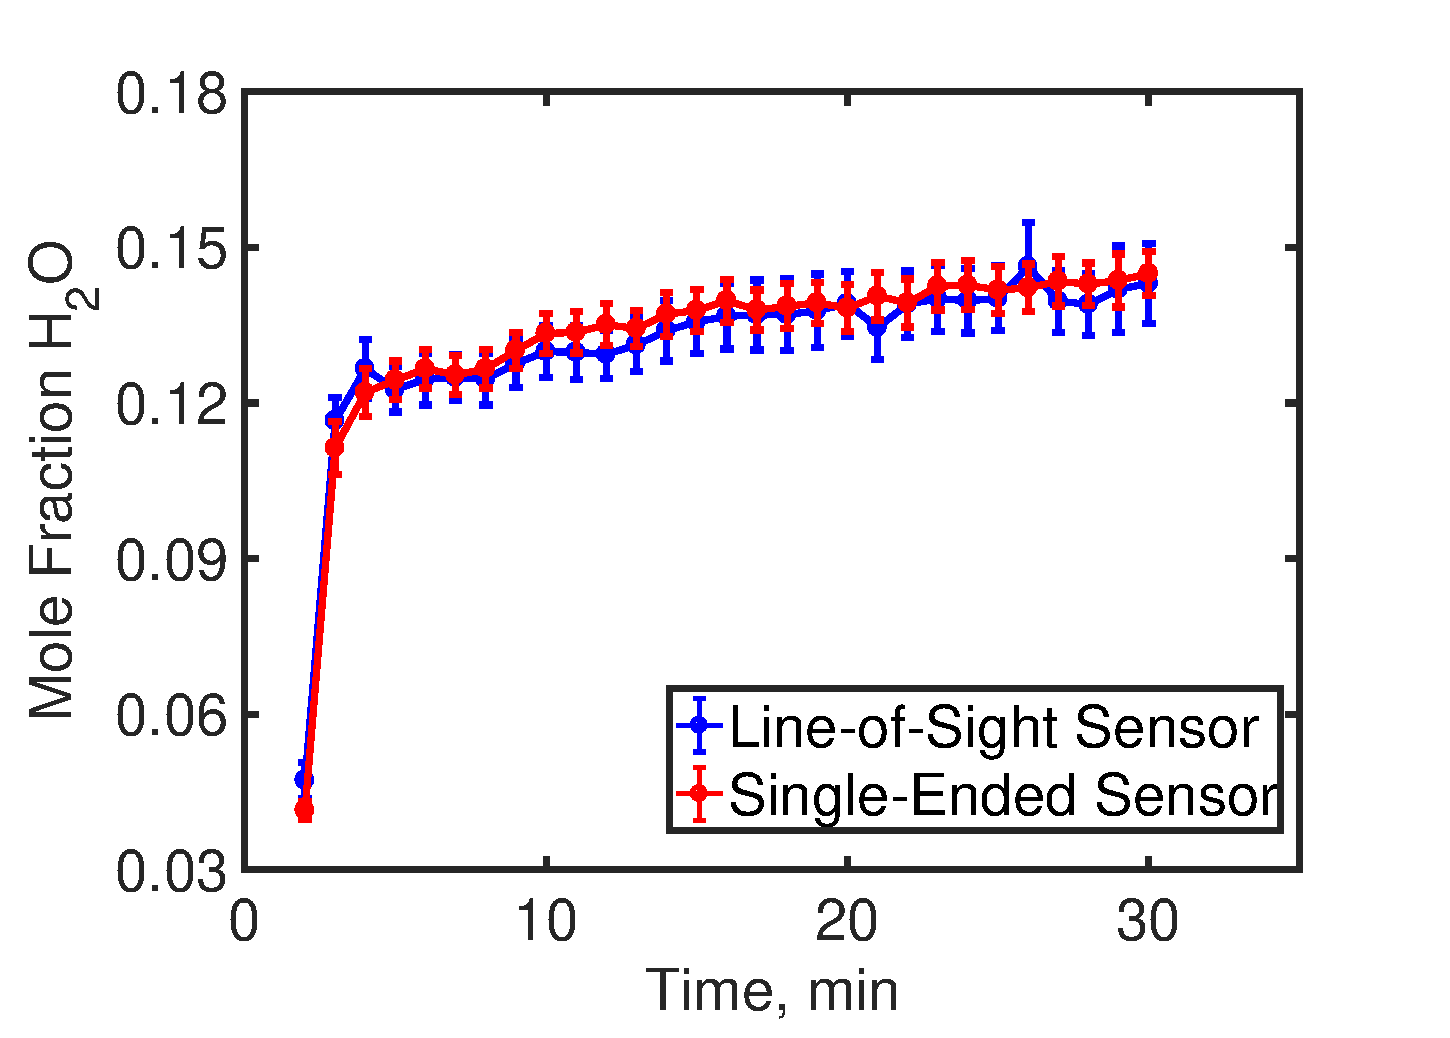
\includegraphics[width=0.7\textwidth]{fig/ch4_fig10_1.eps}  
\caption{Time-averaged (over 1 second) measurements of temperature (left) and $H_2O$ mole fraction (right) acquired using both LAS sensors over a 30 minute period with the burner operating at quasi-steady state. Error bars represent $1\sigma$ variation over each 1-second measurement period. The two LAS sensors agree well over the 30 minute test period and the SE-LAS sensor exhibits superior measurement precision.}
    \label{fig:ch4_10}
\end{figure}


Fig. 4.11 shows time-average (over one second) temperature and $H_2O$ mole fraction measurements acquired by both sensors over the complete 30-minute test period, as well as the burner wall temperature. The error bars represent the $1\sigma$ variation of each quantity within each one-second test. The first two experiments were conducted with the burner throttled to produce a small pilot flame (see Fig. 4.7(b)), and all of the following tests were conducted with the burner operating at full throttle to produce a large swirling flame that filled the burner and measurement path. The results indicate that the burner wall temperature reaches steady-state after 20 minutes and that the gas temperature and $H_2O$ mole fraction also increase slightly for the first 20 minutes of the test. These results can be explained by recognizing that heat transfer losses from the combustion gas will decrease as the burner wall temperature increases which will promote higher gas temperatures and reduce wall quenching. In general, the time-averaged gas temperature and $H_2O$ mole fraction measured by both LAS sensors agree within measurement precision, however the SE-LAS sensor typically recorded a slightly lower ($\approx \,10$-$20$ $K$) temperature. Given that the $H_2O$ mole fractions measured by both LAS sensors remained in agreement throughout the test, the difference in gas temperature is assumed to result from a non-axisymmetric temperature distribution across the measurement plane. This could result from non-axisymmetric heat transfer losses induced by the burner mounting hardware and windows employed by the LOS-LAS sensor.

Over the 30 minute test period the burner wall temperature rose to a temperature of 625 $K$, which provides a conservative estimate for the temperature reached by the SE-LAS sensor’s lens. In addition, the FC/PC to SMA mating sleeve reached a temperature of 80 $C$. The performance of the SE-LAS sensor did not degrade in any observable metric despite its components reaching such high temperatures and its lens being continually exposed to combustion gas at temperatures near 1000 $K$. Optical transmission did not degrade and nor did the signal-to-noise ratio of the WMS-$2f/1f$ signals. Since acquiring the experimental results presented here, similar long-duration experiments have been conducted repeatedly and the SE-LAS sensor has not shown any signs of degradation.

%\include{chap5-engine}
\chapter{SUMMARY AND FUTURE WORK}
\section{Summary}
This thesis presented the design, demonstration, and evaluation of a miniaturized and ruggedized single-ended laser-absorption-spectroscopy (SE-LAS) sensor for measuring gas temperature and $H_2O$ mole fraction in high-temperature combustion environments. The SE-LAS sensor presented here employs a single 6 $mm$ diameter lens, fiber-bundle, and custom body to provide high-fidelity measurements of gas properties while avoiding the use of windows and enabling convenient, alignment-free (after initial assembly) installation in compact locations. Most significantly, it was demonstrated that the SE-LAS sensor can repeatedly withstand direct exposure to high-temperature ($\approx 1000 \,K$) combustion gases for extended periods of time (at least 30 min) without compromising optical throughput or measurement quality. Using wavelength-modulation-spectroscopy techniques, the SE-LAS sensor demonstrated the ability to provide measurements of temperature and $H_2O$ mole fraction at a measurement bandwidth up to 25 $kHz$ and with a precision and accuracy that is comparable to or better than those of a conventional line-of-sight-based LAS sensor. Further, it was shown that the SE-LAS sensor presented here achieved an optical collection efficiency that is comparable (within 0.5$x$) to that of a previously developed SE-LAS sensor which employed an 18x larger-area lens.
In addition, a simple strategy for reducing the computational time required to perform scanned-WMS-$2f/1f$ spectral-fitting was presented. By storing previously calculated scanned-WMS-$2f/1f$ spectra in a look-up library, the best-fit spectra can be determined 100x faster and with an accuracy that is comparable to conventional non-linear least-squares fitting routines that have been used extensively \cite{Goldenstein:16}. This technique enabled the large dataset (240,000 spectra) acquired here to be processed in less than 7 hours instead of 28 days.

\section{Future Work}
\subsection{Field test in an exhaust aftertreatment system}
In Chapter 4, the compact single-ended LAS sensor was demonstrated in a laboratory-scale burner with great precision, accuracy and collection efficiency. In future work, this sensor will be applied to measure temperature and $H_2O$ in a Cummins exhaust aftertreatment system located in the Herrrick Laboratories. The modern diesel exhaust aftertreatment system includes Diesel Oxidation Catalyst (DOC), Diesel Particulate Filters (DPF) and Selective Catalytic Reduction (SCR) catalysts.The DOC and DPF are the first two devices in the aftertreatment system, where DOC oxidizes hydrocarbons, carbon monoxide and unburned fuel, and the DPF filters the remaining soot. SCR system is capable of converting $NO_x$ into water and nitrogen with the aid of urea injection and catalysts. The SCR has been extensively developed and analyzed by many researchers due to its great $NO_x$ reduction efficiency \cite{asif2015urea,southern1993demonstration,recsitouglu2015pollutant,GUAN2014395,doi:10.1177/0142331216656754,qi2003performance,saito2003development,muzio2002overview,gieshoff2000improved,sluder2005low,lei2013influence}. During the operation, the urea decomposes constantly into ammonia ($NH_3$) as the reactant. The reaction temperature will be a critical factor in the performance evaluation of the SCR system due to the high thermal sensitivity of the urea decomposition rate and chemical kinetics. SE-LAS sensors have advantages of taking a non-intrusive and rapid measurement of gas temperature and $H_2O$.

 \begin{figure}[ht]
    \centering       
    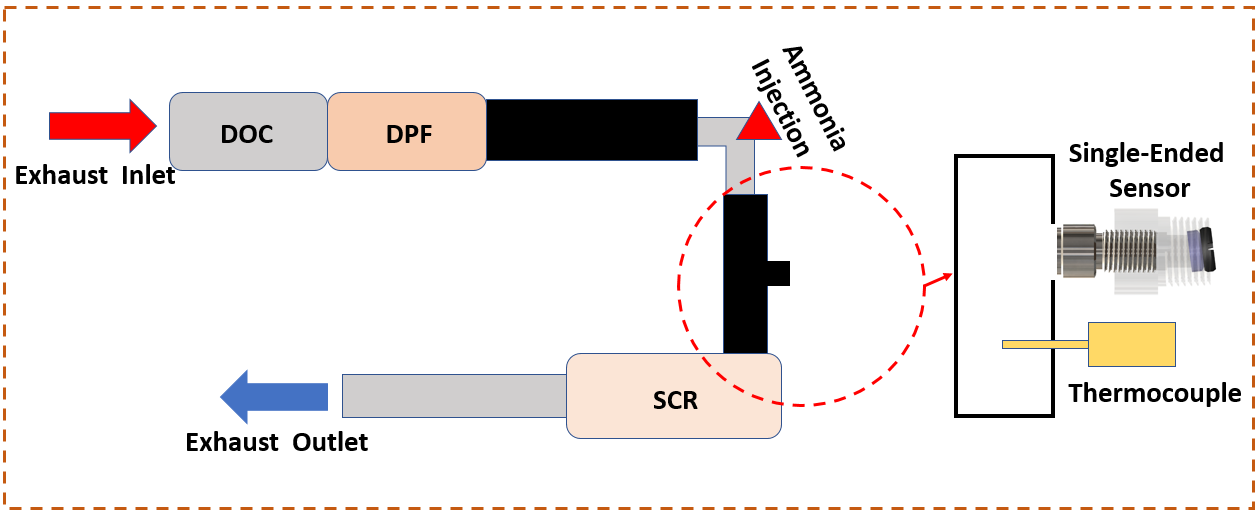
\includegraphics[width=0.8\textwidth]{fig/ch5_fig1.PNG}
        \caption{Schematic of proposed field test of the single-ended temperature and $H_2O$ sensor in the Cummins exhaust aftertreatment system.}
    \label{fig:ch5_1}
\end{figure}

Fig. 5.1 illustrates a schematic of the planned field test with the single-ended sensor in a Cummins exhaust aftertreatment system. The sensor is located upstream of SCR to measure the temperature and $H_2O$ mole fraction with sub-millisecond response time. Furthermore, this sensor can be deployed in more locations (such as downstream of SCR) with/without the urea injection. Several challenges may need to be overcome including: 1) the corrosion on the lens by direct exposure to high-temperature exhaust gas; 2) condensation of $H_2O$ on the lens which could decrease the collection efficiency. 
 


\include{summary}

\include{recommendations}

\bibliography{all}



% Use "\appendix" for one appendix or "\appendices" for more than one
% appendix.
\appendix
\chapter{TECHNICAL DRAWING OF LENS HOUSING IN THE SE-LAS SENSOR}
\begin{figure}
    \centering
        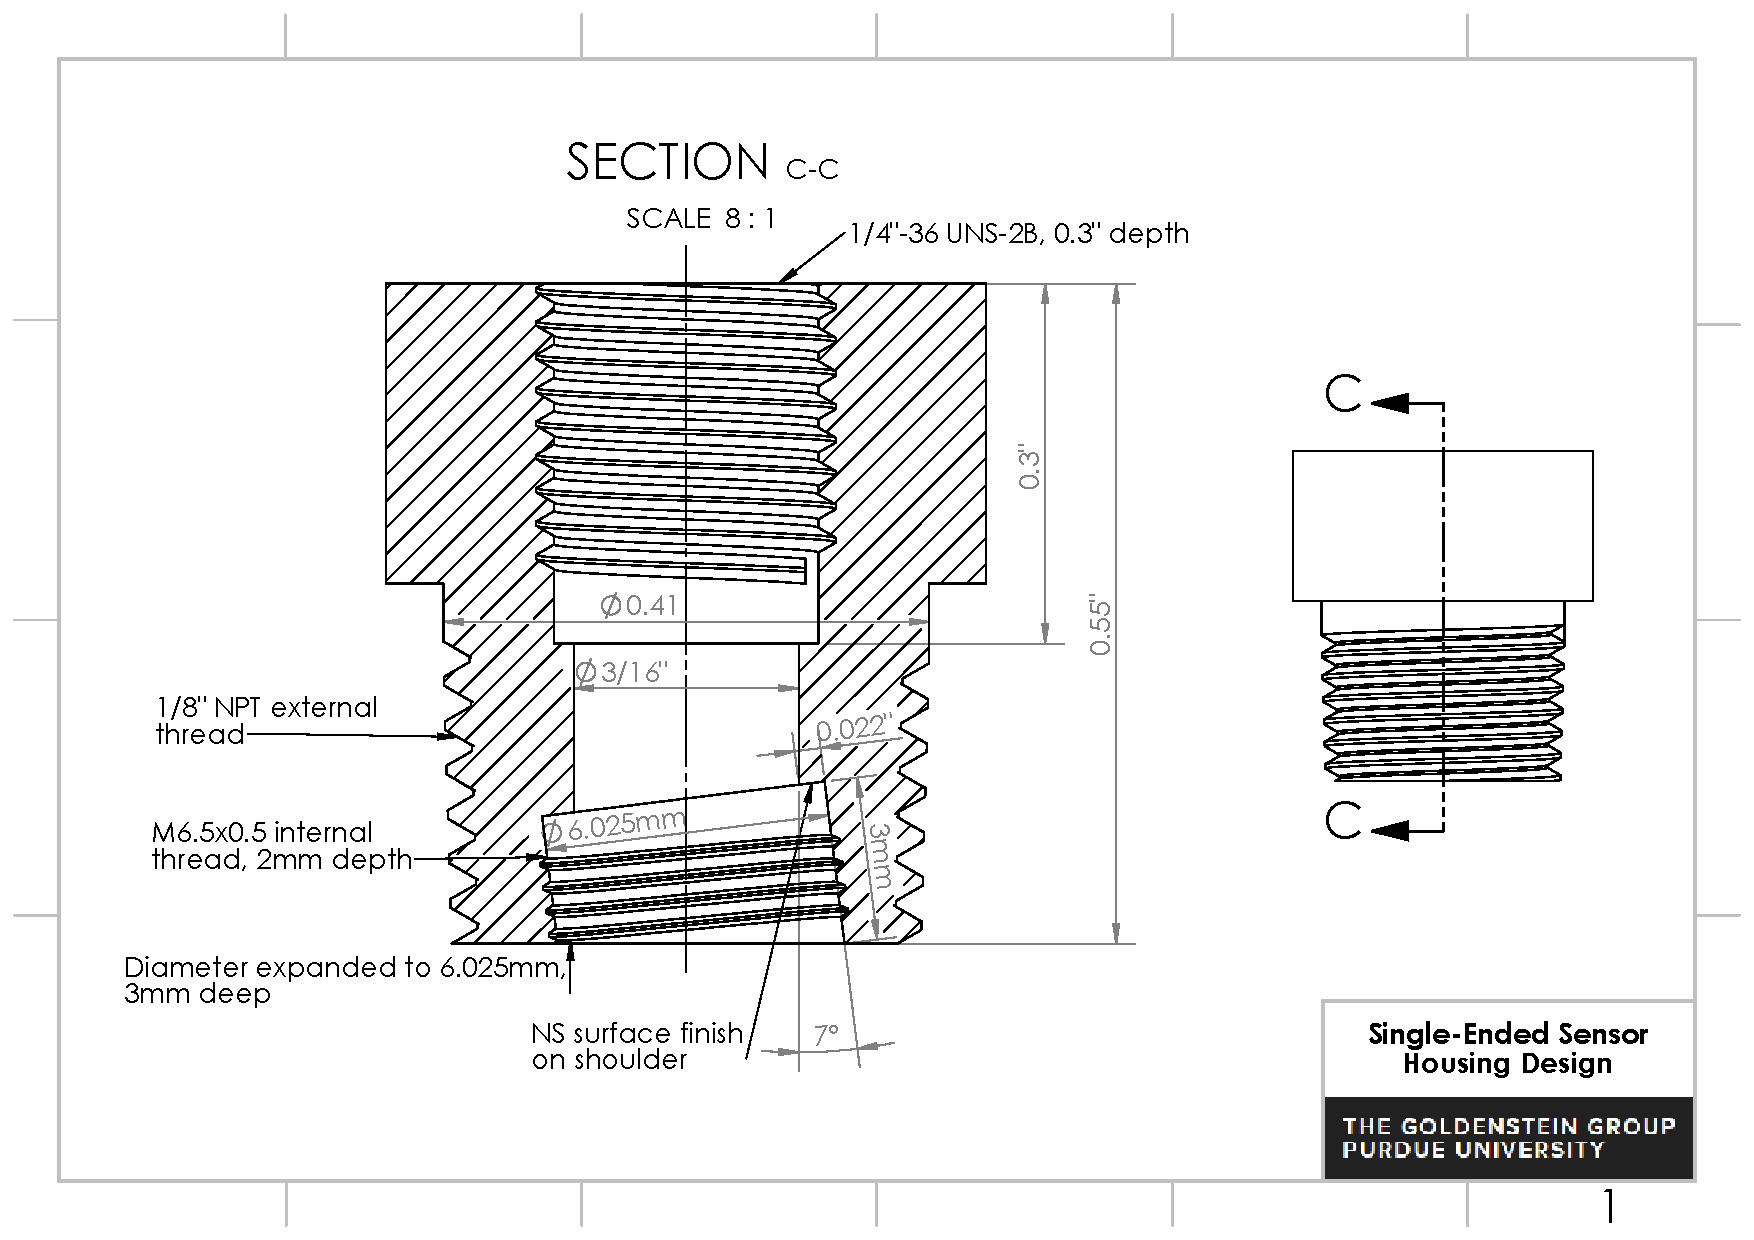
\includegraphics[angle=90,width=1\textwidth]{fig/final1.pdf}      
\end{figure}

\begin{figure}
    \centering
        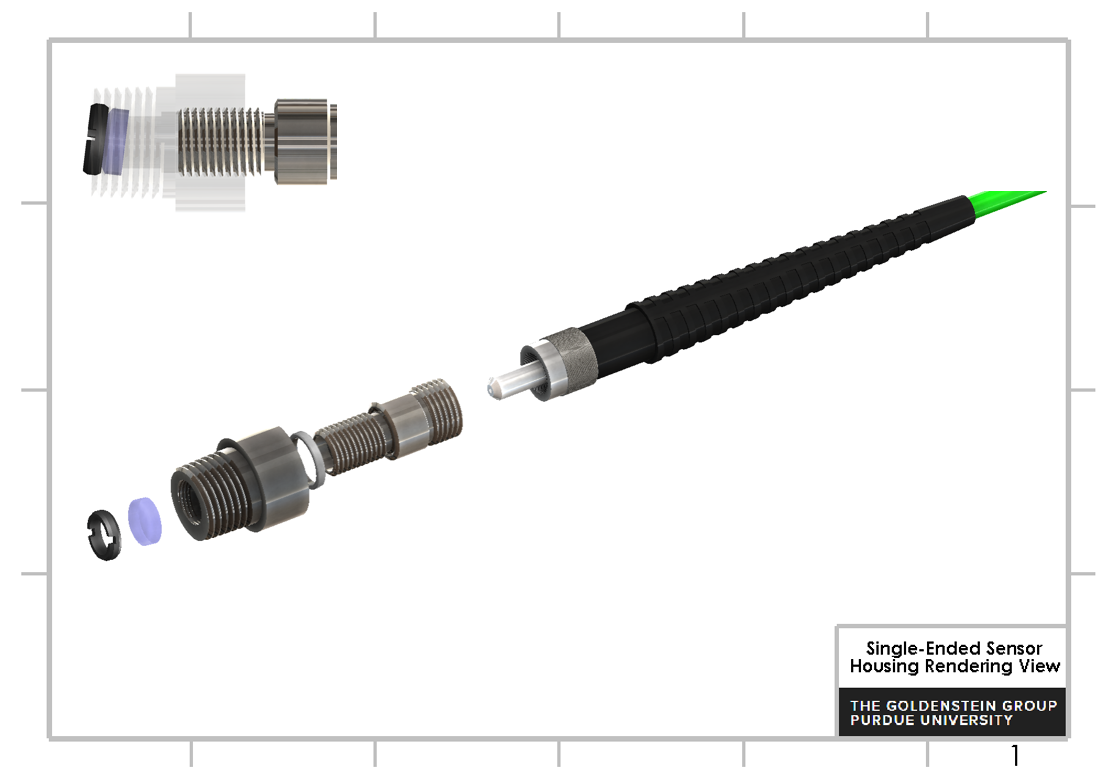
\includegraphics[angle=90,width=1\textwidth]{fig/appendix_v2.png}      
\end{figure}

%\include{demo-citations}
%\include{demo-figures}
%include{demo-multicols}
%\include{demo-tables}
%\include{demo-text}

% A vita is optional for masters theses
% and required for doctoral dissertations.

%\include{vita}

\end{document}